%%%%%%%%%%%%%%%%%%%%%%%%%%%%%%%%%%%%%%%%%%%%%%%%
%
% Strath PhD Thesis Template
%  by Jethro Browell [jethro.browell@strath.ac.uk]
%
%  Guidelines for thesis format, submission and content are found in
%  General and Course Regulations for Graduate and Postgraduate
%  Awards and Degrees, section 20.6.
%
%  Using .eps or .pdf is recomended to prduce high quality figures etc.
%
%  The Strathclyde logo can be found in other formats at www.strath.ac.uk.
%
%%%%%%%%%%%%%%%%%%%%%%%%%%%%%%%%%%%%%%%%%%%%%%%%

\documentclass[a4paper,oneside,11pt]{book}

\usepackage{amsbsy}
\usepackage{amsmath}
\usepackage{amsfonts}
\usepackage{graphicx}
\usepackage{multirow}
\usepackage{mathrsfs}
\usepackage{xcolor}
\usepackage[hidelinks]{hyperref}
\usepackage{cite}
\usepackage{enumitem}
\usepackage{epsfig}
\usepackage{caption}
\usepackage{subcaption}
\usepackage[strict]{changepage}

\usepackage{amssymb}
\usepackage{amsthm}
\usepackage{catchfilebetweentags}
\usepackage[capitalize]{cleveref}
\usepackage{cmll}
\usepackage{ebproof}
\usepackage[utf8]{inputenc}
\usepackage{mathtools}
\usepackage{mathpartir}
\usepackage{multicol}
\usepackage{newunicodechar}
\usepackage{rotating}
\usepackage{stmaryrd}
\usepackage{todonotes}

\usepackage{tikz}
\usetikzlibrary{cd,fit,matrix,positioning}

\usepackage[conor]{agda}

\theoremstyle{definition}
\newtheorem{theorem}{Theorem}[section]
\newtheorem{conjecture}[theorem]{Conjecture}
\newtheorem{proposition}[theorem]{Proposition}
\newtheorem{lemma}[theorem]{Lemma}
\newtheorem{corollary}[theorem]{Corollary}
\newtheorem{example}[theorem]{Example}
\newtheorem{definition}[theorem]{Definition}
\newtheorem{remark}[theorem]{Remark}

\definecolor{use}{HTML}{008000}
\newcommand\gr[1]{{\color{use}#1}}
\newcommand\grctx[1]{\gr{\mathcal{#1}}}
\newcommand\grP{\grctx P}
\newcommand\grQ{\grctx Q}
\newcommand\grR{\grctx R}
\newcommand\grPprime{\grP\gr'}
\newcommand\grQprime{\grQ\gr'}
\newcommand\grRprime{\grR\gr'}
\newcommand\name{\ensuremath{\lambda\grR}}
\newcommand\grctxsub[2]{\grctx{#1}_{\gr{#2}}}
\newcommand\grPe{\grctxsub P e}
\newcommand\grPf{\grctxsub P f}
\newcommand\grPl{\grctxsub P l}
\newcommand\grPr{\grctxsub P r}
\newcommand\grQe{\grctxsub Q e}
\newcommand\grQf{\grctxsub Q f}
\newcommand\grQl{\grctxsub Q l}
\newcommand\grQr{\grctxsub Q r}
\newcommand\grRl{\grctxsub R l}
\newcommand\grRr{\grctxsub R r}
\newcommand\ps{\mathit{ps}}
\newcommand\qs{\mathit{qs}}
\newcommand\rs{\mathit{rs}}
\newcommand\dotto{\mathrel{\dot\to}}
\newcommand\dotlr{\mathrel{\dot\leftrightarrow}}
\newcommand\dottimes{\mathbin{\dot\times}}
%\newcommand\dotplus{\mathbin{\dot+}}
\newcommand\wand{\mathrel{\mathord{-}\hspace{-0.75ex}*}}
\newcommand\sep{\mathbin{*}}
\newcommand\Boxzp{\Box^{0{+}}}
\newcommand\Boxzpt{\Box^{0{+}{*}}}
\providecommand\U{}
\renewcommand\U{\mathcal U}
\newcommand\V{\mathcal V}
\newcommand\W{\mathcal W}
\providecommand\C{}
\renewcommand\C{\mathcal C}
\newcommand\sqin{\mathrel{\mathrlap{\sqsubset}{\mathord{-}}}}
\newcommand\sqni{\mathrel{\mathrlap{\sqsupset}{\mathord{-}}}}
\newcommand\Ann{\mathscr R}

\renewcommand\land{~\wedge~}
\renewcommand\lor{~\vee~}
\newcommand\rel{\mathrel{\mathord{\to}\hspace{-2.25ex}+}}

\DeclareMathOperator\Set{Set}
\DeclareMathOperator\obj{Obj}
\DeclareMathOperator\List{List}
\let\hom\relax
\DeclareMathOperator\hom{Hom}
\DeclareMathOperator\id{id}
\DeclareMathOperator\sub{Sub}

\newcommand\env[1]{\stackrel{#1}\Longrightarrow}

\usepackage{mleftright}
\newcommand\lr[3]{\mleft#1{#2}\mright#3}
\newcommand\sem[1]{\lr\llbracket{#1}\rrbracket}
\newcommand\size[1]{\lr\lvert{#1}\rvert}
\newcommand\plr[1]{\lr({#1})}
\newcommand\blr[1]{\lr[{#1}]}
\newcommand\forallb[1]{\forall\blr{~#1~}}
\newcommand\alr[1]{\lr\langle{#1}\rangle}
\newcommand\bra[1]{\lr\langle{#1}\rvert}
\newcommand\ket[1]{\lr\lvert{#1}\rangle}

\newcommand\leO{\;{\leq}0}
\newcommand\leI{\;{\leq}1}

\DeclareMathOperator{\lin}{lin}
\DeclareMathOperator{\intu}{int}
\newcommand\lnl{\ensuremath{\mathrm{L/nL}}}
\newcommand\vdashL{\mathrel{\vdash_{\mathcal L}}}
\newcommand\vdashC{\mathrel{\vdash_{\mathcal C}}}

\ebproofnewstyle{comb}{separation=0.75em}
\ebproofset{right label template=\TirName{\inserttext}}

\newenvironment{eqns}{\begin{array}{r@{\hspace{0.3em}}c@{\hspace{0.3em}}l}}{\end{array}}

\newcommand\PsiDot[1]{%
  \AgdaBound{$\Psi$}\AgdaSpace{}\AgdaSymbol{.}\AgdaField{#1}}

\newcommand\qto{\mathbin{`\!\to}}

\newcommand\Lock{\text{\faLock}}

\newcommand\oiw{\mathrm{\gr{01\upomega}}}

\newcommand\colour{%
{\color{AgdaField}co}{\color{AgdaFunction}lo}{\color{AgdaDatatype}ur}%
}

\usepackage[T1]{fontenc}

\newunicodechar{λ}{\ensuremath{\mathnormal\lambda}}
\newunicodechar{ρ}{\ensuremath{\mathnormal\rho}}
\newunicodechar{→}{\ensuremath{\mathnormal\to}}
\newunicodechar{∀}{\ensuremath{\mathnormal\forall}}
\newunicodechar{∃}{\ensuremath{\mathnormal\exists}}
\newunicodechar{ι}{\ensuremath{\mathnormal\iota}}
\newunicodechar{·}{\ensuremath{\mathnormal\cdot}}
\newunicodechar{⊸}{\ensuremath{\mathnormal\multimap}}
\newunicodechar{⊕}{\ensuremath{\mathnormal\oplus}}
\newunicodechar{⊗}{\ensuremath{\mathnormal\otimes}}
\newunicodechar{⅋}{\ensuremath{\mathnormal\parr}}
\newunicodechar{─}{\text{---}}
\newunicodechar{│}{\ensuremath{\mid}}
\newunicodechar{ᶜ}{\ensuremath{\mathnormal{^c}}}
\newunicodechar{ᵉ}{\ensuremath{\mathnormal{^e}}}
\newunicodechar{ᵏ}{\ensuremath{\mathnormal{^k}}}
\newunicodechar{ₗ}{\ensuremath{\mathnormal{_l}}}
\newunicodechar{ₘ}{\ensuremath{\mathnormal{_m}}}
\newunicodechar{ₙ}{\ensuremath{\mathnormal{_n}}}
\newunicodechar{ᵣ}{\ensuremath{\mathnormal{_r}}}
\newunicodechar{ʳ}{\ensuremath{\mathnormal{^r}}}
\newunicodechar{ˢ}{\ensuremath{\mathnormal{^s}}}
\newunicodechar{ᵗ}{\ensuremath{\mathnormal{^t}}}
\newunicodechar{ᵛ}{\ensuremath{\mathnormal{^v}}}
\newunicodechar{ʷ}{\ensuremath{\mathnormal{^w}}}
\newunicodechar{ᴹ}{\ensuremath{\mathnormal{^M}}}
\newunicodechar{ᴿ}{\ensuremath{\mathnormal{^R}}}
\newunicodechar{↙}{\ensuremath{\mathnormal\swarrow}}
\newunicodechar{↘}{\ensuremath{\mathnormal\searrow}}
\newunicodechar{⊢}{\ensuremath{\mathnormal\vdash}}
\newunicodechar{⊨}{\ensuremath{\mathnormal\vDash}}
\newunicodechar{⟦}{\ensuremath{\mathnormal\llbracket}}
\newunicodechar{⟧}{\ensuremath{\mathnormal\rrbracket}}
\newunicodechar{✴}{\ensuremath{\mathnormal*}}
\newunicodechar{ℓ}{\ensuremath{\mathnormal\ell}}
\newunicodechar{α}{\ensuremath{\mathnormal\alpha}}
\newunicodechar{Γ}{\ensuremath{\mathnormal\Gamma}}
\newunicodechar{γ}{\ensuremath{\mathnormal\gamma}}
\newunicodechar{Δ}{\ensuremath{\mathnormal\Delta}}
\newunicodechar{δ}{\ensuremath{\mathnormal\delta}}
\newunicodechar{ε}{\ensuremath{\mathnormal\epsilon}}
\newunicodechar{Θ}{\ensuremath{\mathnormal\Theta}}
\newunicodechar{μ}{\ensuremath{\mathnormal\mu}}
\newunicodechar{Σ}{\ensuremath{\mathnormal\Sigma}}
\newunicodechar{σ}{\ensuremath{\mathnormal\sigma}}
\newunicodechar{ω}{\ensuremath{\mathnormal\omega}}
\newunicodechar{∈}{\ensuremath{\mathnormal\in}}
\newunicodechar{′}{\ensuremath{\mathnormal'}}
\newunicodechar{≡}{\ensuremath{\mathnormal\equiv}}
\newunicodechar{⊤}{\ensuremath{\mathnormal\top}}
\newunicodechar{⊥}{\ensuremath{\mathnormal\bot}}
\newunicodechar{▹}{\ensuremath{\mathnormal\triangleright}}
\newunicodechar{₁}{\ensuremath{\mathnormal{_1}}}
\newunicodechar{□}{\ensuremath{\mathnormal\Box}}
\newunicodechar{○}{\ensuremath{\mathnormal\bigcirc}}
\newunicodechar{𝓒}{\ensuremath{\C}}
\newunicodechar{𝓥}{\ensuremath{\V}}
\newunicodechar{∘}{\ensuremath{\mathnormal\circ}}
\newunicodechar{≤}{\ensuremath{\mathnormal\leq}}
\newunicodechar{◇}{\ensuremath{\mathnormal\diamond}}
\newunicodechar{ℕ}{\ensuremath{\mathbb N}}
\newunicodechar{ℤ}{\ensuremath{\mathbb Z}}
\newunicodechar{⁺}{\ensuremath{\mathnormal{^+}}}
\newunicodechar{⁻}{\ensuremath{\mathnormal{^-}}}
\newunicodechar{⊔}{\ensuremath{\mathnormal\sqcup}}
\newunicodechar{⇒}{\ensuremath{\mathnormal\Rightarrow}}
\newunicodechar{Ψ}{\ensuremath{\mathnormal\Psi}}
\newunicodechar{⋯}{\ensuremath{\mathnormal\cdots}}
\newunicodechar{∞}{\ensuremath{\mathnormal\infty}}
\newunicodechar{≈}{\ensuremath{\mathnormal\approx}}
\newunicodechar{⟨}{\ensuremath{\mathnormal\langle}}
\newunicodechar{⟩}{\ensuremath{\mathnormal\rangle}}
\newunicodechar{∣}{\ensuremath{\mathnormal\vert}}
\newunicodechar{⋂}{\ensuremath{\mathnormal\bigcap}}
\newunicodechar{∙}{\ensuremath{\mathnormal\bullet}}
\newunicodechar{∼}{\ensuremath{\mathnormal\sim}}

% Characters that are different from what appears in the source code
\newunicodechar{∋}{\ensuremath{\mathnormal\sqni}}
\newunicodechar{ℑ}{\ensuremath{\mathnormal{I^*}}}
\newunicodechar{⇛}{\ensuremath{\mathnormal{\Longrightarrow}}}
\newunicodechar{∩}{\ensuremath{\mathnormal\dottimes}}
\newunicodechar{∧}{\ensuremath{\mathnormal\dottimes}}
\newunicodechar{⒈}{\ensuremath{\mathnormal{\dot1}}}
\newunicodechar{⇴}{\ensuremath{\mathnormal\dotto}}
\newunicodechar{⇥}{\ensuremath{\mathnormal\wand}}


% Page Margins - Strath Requirement
\usepackage[left=4cm,right=2.5cm,top=2cm,bottom=4cm,includehead,includefoot,headheight=15pt]{geometry}

% Page Headers
\usepackage{fancyhdr}
\fancyhf{}
\renewcommand{\headrulewidth}{0pt} % optional
%\fancyhead[L]{\nouppercase{\leftmark} \hfill Section \nouppercase{\rightmark}}
\fancyhead[L]{\nouppercase{\leftmark}}
\cfoot{\thepage}
\pagestyle{fancy}

% Draft Watermark
%\usepackage[draft=true,allpages=true,fontfamily=cmr,angle=90,scale=0.1,mark={\fboxsep=35pt\fboxrule=0pt\relax\fbox{-- DRAFT -- \today~--}},xcoord=-80,ycoord=-20]{draftwatermark}


% Line Spacing
%\def\baselinestretch{1.5}
\usepackage{setspace}
\setstretch{1.5}


% Place UoS Logo on Title Page (this package modifies the "\maketitel" command.)
\usepackage{titling}
\pretitle{%
  \begin{flushright}
  \vspace{-9.5cm}
%  
\includegraphics[width=5cm,natwidth=472,natheight=531]{logo} \\[7cm]
  
\includegraphics[width=5cm]{logo} \\[6cm]
  \end{flushright}
  \begin{center}
  \LARGE
}
\posttitle{\end{center}}

\title{PhD Title \\ PhD Thesis}
\author{James Wood
\\ \small Mathematically Structured Programming\\[-0.8ex]
\small Computer and Information Sciences\\[-0.8ex]
\small University of Strathclyde, Glasgow\\
}




%%%%%%%%%%%%%%%%%%%%%%%%%%%%%%%%%%%%%%%%%%%%%%%%%%%%%%%%%%%%%%
\begin{document}

\maketitle


%%%%%%%%%%%%%%%%%%%%%%%%%%%%%%%%%%%%%%%%%%%%%%%%%%%%%%%%%%%%%%
\frontmatter
%%%%%%%%%%%%%%%%%%%%%%%%%%%%%%%%%%%%%%%%%%%%%%%%%%%%%%%%%%%%%%

% Declaration
\topskip0pt
\vspace*{\fill}
\noindent
\begin{quote}
  \centering
  This thesis is the result of the author's original research. It has been composed by the author and has not been previously submitted for examination which has led to the award of a degree. \\[5pt]
  %
  The copyright of this thesis belongs to the author under the terms of the United Kingdom Copyright Acts as qualified by University of Strathclyde Regulation 3.50. Due acknowledgement must always be made of the use of any material contained in, or derived from, this thesis. \\[5pt]
  %
  %Signed: \\
  %Date:
\end{quote}
\vspace*{\fill}



\chapter{Abstract}



\tableofcontents

\addcontentsline{toc}{chapter}{List of Figures}
\listoffigures

\addcontentsline{toc}{chapter}{List of Tables}
\listoftables



\chapter{Preface/Acknowledgements}
I would like to acknowledge...

This document is adapted from the template by Jethro Browell
(\url{https://www.overleaf.com/latex/templates/thesis-template-for-university-of-strathclyde/nfnrnmjqyxqg}),
which was licensed under CC BY 4.0.



%%%%%%%%%%%%%%%%%%%%%%%%%%%%%%%%%%%%%%%%%%%%%%%%%%%%%%%%%%%%%%
\mainmatter
%%%%%%%%%%%%%%%%%%%%%%%%%%%%%%%%%%%%%%%%%%%%%%%%%%%%%%%%%%%%%%


\chapter{Introduction}

\chapter{Mathematical preliminaries}
  Categories, (co)products, monoidal categories, string diagrams (in Rel),
  monoid objects.
  Examples: Set, Rel, partial functions, commutative monoids.

\chapter{Linearity}
  \section{Intuitionistic linear logic}
  Linear logic is a good starting point for our investigations into usage
restrictions because it is well known, well understood, and exhibits most of the
difficulties we will come across.
Linear logic's lack of general weakening and contraction will be a typical
feature of the calculi we will see, and the exponential modality $\oc$ (bang)
will be the prototype for a range of modalities I will consider.

\subsection{Motivation of linearity}

While classical linear logic is perhaps better understood, for the sake of this
thesis I focus on intuitionistic linear logic.
The syntactic difference between the two is analogous to the difference between
classical and intuitionistic logic: The latter restricts the former by only
allowing one formula on the right of a sequent.
Classical linear logic is not irrelevant to this thesis, and appears as an
instance of the framework presented in \cref{sec:framework}.
However, the connection of this work to intuitionistic linear logic is more
direct, and reflects the basis of existing semiring-annotated calculi on
(intuitionistic) typed $\lambda$-calculi.

Intuitionistic linear logic is often motivated by its sensitivity to resources.
The fact that, in intuitionistic (and classical) logic, \emph{any} hypothesis
can be discarded or duplicated means that propositions cannot be used to model
things that may be ``possessed'' or ``spent'', despite hypotheses often being
described as things we ``have''.
In contrast, linear logic allows propositions to behave like physical objects,
being moved around but not being created or destroyed (a priori).

Programming applications of linearity include stateful protocols
\citep{Wadler12}, mutually exclusive capabilities (TODO: cite),
and mutation (TODO: cite).
In each of these cases, the act of using up a hypothesis allows us to divide
time into ``before'' and ``after'', with lack of duplication avoiding confusion
over which half we are in, and lack of deletion allowing us to know whether the
corresponding action actually happened.
For example, when modelling mutation, a variable refers to a single state of a
mutable value.
The \texttt{write} operation uses up such a variable, making the old state
inaccessible, and returns a new linear value to represent the new state of the
mutable value.
Such a protocol naturally also supports a \emph{freezing} operation, by which we
relinquish the ability to mutate the value in return for an immutable reference
to the value produced.

%In LJ, two distinct, but equiderivable, canonical definitions of $\wedge$ can
%be given.
%
%In the first approach, $\wedge^-$ is conceived to be a
%\emph{categorial product}.
%Such a product is constructed by providing two maps in from the same antecedents
%$\Gamma$.
%It is used by projecting out one of the sides.
%
%\begin{mathpar}
%  \inferrule*[right=$\wedge^-$-r]
%  {\Gamma \vdash A \\ \Gamma \vdash B}
%  {\Gamma \vdash A \wedge^- B}
%
%  \and
%
%  \inferrule*[right=$\wedge^-$-l$_0$]
%  {\Gamma, A \vdash C}
%  {\Gamma, A \wedge^- B \vdash C}
%
%  \and
%
%  \inferrule*[right=$\wedge^-$-l$_1$]
%  {\Gamma, B \vdash C}
%  {\Gamma, A \wedge^- B \vdash C}
%\end{mathpar}
%
%In the second approach, $\wedge^+$ is conceived to be a \emph{tensor product}.
%Intuitively, $\wedge^+$ internalises the comma of context concatenation.
%Such a product is used by giving access to both sides simultaneously.
%It is constructed by constructing both sides and combining the antecedents
%required by each side.
%
%\begin{mathpar}
%  \inferrule*[right=$\wedge^+$-r]
%  {\Gamma \vdash A \\ \Delta \vdash B}
%  {\Gamma, \Delta \vdash A \wedge^+ B}
%
%  \and
%
%  \inferrule*[right=$\wedge^+$-l]
%  {\Gamma, A, B \vdash C}
%  {\Gamma, A \wedge^+ B \vdash C}
%\end{mathpar}
%
%When we prove the logical equivalence of these two formulations, we notice that
%the structural rules of weakening and contraction are essential.
%When we remove weakening and contraction, $\wedge^-$ and $\wedge^+$ become
%logically distinct connectives, which we notate $\&$ and $\otimes$,
%respectively.
%
%\begin{mathpar}
%  \inferrule*[right=$\wedge^-$-r]
%  {%
%    \inferrule*[right=Weak$^*$,fraction={\cdot\cdots\cdot}]
%    {\Gamma \vdash A}
%    {\Gamma, \Delta \vdash A}
%    \\
%    \inferrule*[Right=Weak$^*$,fraction={\cdot\cdots\cdot}]
%    {\Delta \vdash B}
%    {\Gamma, \Delta \vdash B}
%  }
%  {\Gamma, \Delta \vdash A \wedge^- B}
%
%  \and
%
%  \inferrule*[right=Contr]
%  {%
%    \inferrule*[Right=$\wedge^-$-l$_0$]
%    {%
%      \inferrule*[Right=$\wedge^-$-l$_1$]
%      {\Gamma, A, B \vdash C}
%      {\Gamma, A, A \wedge^- B \vdash C}
%    }
%    {\Gamma, A \wedge^- B, A \wedge^- B \vdash C}
%  }
%  {\Gamma, A \wedge^- B \vdash C}
%\end{mathpar}
%
%\begin{mathpar}
%  \inferrule*[right=Contr$^*$,fraction={\cdot\cdots\cdot}]
%  {%
%    \mprset{defaultfraction}
%    \inferrule*[Right=$\wedge^+$-r]
%    {\Gamma \vdash A \\ \Gamma \vdash B}
%    {\Gamma, \Gamma \vdash A \wedge^+ B}
%  }
%  {\Gamma \vdash A \wedge^+ B}
%
%  \and
%
%  \inferrule*[right=$\wedge^+$-l]
%  {%
%    \inferrule*[Right=Weak]
%    {\Gamma, A \vdash C}
%    {\Gamma, A, B \vdash C}
%  }
%  {\Gamma, A \wedge^+ B \vdash C}
%
%  \and
%
%  \inferrule*[right=$\wedge^+$-l]
%  {%
%    \inferrule*[Right=Weak]
%    {\Gamma, B \vdash C}
%    {\Gamma, A, B \vdash C}
%  }
%  {\Gamma, A \wedge^+ B \vdash C}
%\end{mathpar}

\subsection{The multiplicative-additive fragment}

The multiplicative-additive fragment of linear logic (MALL) is the fragment
where all hypotheses are linear (must be used exactly once).
We will extend MALL with the \emph{exponential} modality in
\cref{sec:bang-modality}.
MALL is unable to embed intuitionistic or classical logic (collectively
known as \emph{structural logics}), as MALL is unable to reflect any of the
discarding or duplication that can be done in proofs in structural logics.

In short, the syntax of intuitionistic MALL can be described as intuitionistic
logic with the structural rules of \emph{weakening} and \emph{contraction}
removed.
However, without the presence of weakening and contraction, we have to be more
careful about the rules we state, so as not to accidentally introduce weakening
and contraction admissibly.
The lack of these structural rules also allows us to observe a new phenomenon:
the distinction (at the level of provability) between \emph{additive} and
\emph{multiplicative} formulations of existing connectives (in particular, in
the intuitionistic case, the conjunction connective).

I present MALL in \cref{fig:mall} in a sequent calculus style, as it was
presented by \citet{girard87linear}.

To encode what it means to use a hypothesis \emph{exactly once}, we first need
to decide what counts as a use.
The simplest case is that the identity sequent counts as a single use of its
sole hypothesis, and conversely does not count as a use of any other hypotheses.
For sequential proofs, created by the \TirName{Cut} rule, if we have a proof of
$A$ using $\Gamma$, and a proof of $B$ using $\Delta$ and $A$, then we have a
proof of $B$ transitively using $\Delta$ and $\Gamma$.
The exchange rule Exch says that use is invariant under permutation.

For the logical connectives, we have genuine choices as to what it means to use
them.
Two cases --- disjunction ($\oplus$) and (linear) implication ($\multimap$) ---
are somewhat intuitive from intuitionistic logic.
A canonical proof of a disjunction is a tag and a proof of one of the two
disjuncts.
This suggests that a proof of a disjunction only uses the same hypotheses as
the proof of the disjunct we actually choose, with the other disjunct being
irrelevant.
Correspondingly, when we use a disjunction hypothesis, we will only actually use
one of the cases, so each branch should use the same hypotheses.
For implication, use is sequential like with the \TirName{Cut} rule, and its
left rule is more or less the only choice that allows use of the surrounding
hypotheses.

For conjunction, there are two choices: Either the conjuncts \emph{together} use
all of the hypotheses, or each of the conjuncts \emph{individually} uses all of
the hypotheses.
The former choice gives us the tensor-product ($\otimes$), and the latter choice
gives us the with-product ($\with$).
These products are equivalent up to provability in structural logics but
distinct in linear logic.

\begin{figure}
  \begin{align*}
    A, B, C &\Coloneqq X \mid I \mid A \otimes B \mid A \multimap B
              \mid 0 \mid A \oplus B \mid \top \mid A \with B \\
    \Gamma, \Delta, \Theta &\Coloneqq {\cdot} \mid \Gamma, A
  \end{align*}
  \begin{mathpar}
    \ebrule{%
      \infer0[Id]{A \vdash A}
    }

    \and

    \ebrule{%
      \hypo{\Gamma \vdash A}
      \hypo{\Delta, A \vdash B}
      \infer2[Cut]{\Gamma, \Delta \vdash B}
    }

    \and

    \ebrule{%
      \hypo{\Gamma, B, A, \Delta \vdash C}
      \infer1[Exch]{\Gamma, A, B, \Delta \vdash C}
    }

    \and

    \ebrule{%
      \hypo{\Gamma \vdash C}
      \infer1[$I$-L]{\Gamma, I \vdash C}
    }

    \and

    \ebrule{%
      \infer0[$I$-R]{{\cdot} \vdash I}
    }

    \and

    \ebrule{%
      \hypo{\Gamma, A, B \vdash C}
      \infer1[$\otimes$-L]{\Gamma, A \otimes B \vdash C}
    }

    \and

    \ebrule{%
      \hypo{\Gamma \vdash A}
      \hypo{\Delta \vdash B}
      \infer2[$\otimes$-R]{\Gamma, \Delta \vdash A \otimes B}
    }

    \and

    \ebrule{%
      \hypo{\Gamma \vdash A}
      \hypo{\Delta, B \vdash C}
      \infer2[$\multimap$-L]{\Gamma, \Delta, A \multimap B \vdash C}
    }

    \and

    \ebrule{%
      \hypo{\Gamma, A \vdash B}
      \infer1[$\multimap$-R]{\Gamma \vdash A \multimap B}
    }

    \and

    \ebrule{%
      \infer0[$0$-L]{\Gamma, 0 \vdash C}
    }

    \and

    \text{(no $0$-R)}

    \and

    \ebrule{%
      \hypo{\Gamma, A \vdash C}
      \hypo{\Gamma, B \vdash C}
      \infer2[$\oplus$-L]{\Gamma, A \oplus B \vdash C}
    }

    \and

    \ebrule{%
      \hypo{\Gamma \vdash A_i}
      \infer1[$\oplus$-R$_i$]{\Gamma \vdash A_0 \oplus A_1}
    }

    \and

    \text{(no $\top$-L)}

    \and

    \ebrule{%
      \infer0[$\top$-R]{\Gamma \vdash \top}
    }

    \and

    \ebrule{%
      \hypo{\Gamma, A_i \vdash C}
      \infer1[$\with$-L$_i$]{\Gamma, A_0 \with A_1 \vdash C}
    }

    \and

    \ebrule{%
      \hypo{\Gamma \vdash A}
      \hypo{\Gamma \vdash B}
      \infer2[$\with$-R]{\Gamma \vdash A \with B}
    }
  \end{mathpar}
  \caption{Multiplicative-additive fragment of linear logic}
  \label{fig:mall}
\end{figure}

Implication ($\multimap$) and the tensor-product ($\otimes$, $I$) comprise the
\emph{multiplicative} fragment, while disjunction ($\oplus$, $0$) and the
with-product ($\with$, $\top$) comprise the \emph{additive} fragment.
Categorically, the additive fragment corresponds to products and coproducts,
while the multiplicative fragment corresponds to multicategorical tensor
products and closure.

\subsection{The $\oc$-modality}\label{sec:bang-modality}

\begin{mathpar}
  \ebrule{%
    \hypo{\oc\Gamma \vdash A}
    \infer1[Promotion]{\oc\Gamma \vdash \oc A}
  }

  \and

  \ebrule{%
    \hypo{\Gamma, A \vdash B}
    \infer1[Dereliction]{\Gamma, \oc A \vdash B}
  }

  \and

  \ebrule{%
    \hypo{\Gamma \vdash B}
    \infer1[Weakening]{\Gamma, \oc A \vdash B}
  }

  \and

  \ebrule{%
    \hypo{\Gamma, \oc A, \oc A \vdash B}
    \infer1[Contraction]{\Gamma, \oc A \vdash B}
  }
\end{mathpar}

In the intuitionistic linear logic sequent calculus ILL, $\oc A$ is defined
to be a proposition whose occurrences as antecedents can be deleted
(\TirName{Weakening}) and duplicated (\TirName{Contraction}), from which we can
extract $A$ (\TirName{Dereliction}), and which we can form from a conclusion
$A$ only when all antecedents are of the form $\oc X$ for some proposition $X$
(\TirName{Promotion}).
In short, $\oc A$ can be seen as an intuitionistic version of $A$, supporting
all of the structural rules of LJ, and only being able to be formed when it
does not depend on anything linear.

While this definition of $\oc$ works, in the sense that it gives the intended
class of models and cut elimination is maintained, it has some disadvantages.
Firstly, while the multiplicative and additive connectives are all characterised
by universal properties, $\oc$ is not.
This can be seen by the fact that taking the rules for $\oc$ and replacing each
occurrence of $\oc$ by a fresh connective $\oc'$ produces a logically distinct
connective.
One cannot produce any derivation of $\oc' A \vdash \oc A$ because
\TirName{Promotion} does not apply when there are antecedents not of the form
$\oc X$.
Finally, while $\oc$ is supposed to be a positive connective, it sometimes
behaves like a negative connective.
For example, for a positive connective like $\otimes$, the normal form proof
of the identity sequent $P \otimes Q \vdash P \otimes Q$ starts (from the
bottom) with a left rule and then, with the left in a more amenable form,
applies the right rule.
In contrast, the normal form proof of $\oc P \vdash \oc P$ starts with the
right rule, as it needs to have everything on the left be of the form $\oc X$.

\begin{mathpar}
  \ebrule{%
    \infer0[Id]{P \vdash P}
    \infer0[Id]{Q \vdash Q}
    \infer2[$\otimes$-r]{P, Q \vdash P \otimes Q}
    \infer1[$\otimes$-l]{P \otimes Q \vdash P \otimes Q}
  }

  \and

  \ebrule{%
    \infer0[Id]{P \vdash P}
    \infer1[Der]{\oc P \vdash P}
    \infer1[Pro]{\oc P \vdash \oc P}
  }
\end{mathpar}

  \section{DILL}
  DILL provides a syntax in which $\oc$ is characterised by a universal
  property.
  There is no need for any rule to depend on the entire context and rebind
  variables (as done by BBdPH), so is more ND-like.
  DILL makes $\oc$ behave more like a positive type former (see the deep
  identity function $\oc A \vdash \oc A$).
  DILL has been extended to dependent types: Vakar15.

  The idea of split contexts can also be applied to left-/right-rule systems.
  (Define this DILL variant.)

  \section{Mechanisation survey}

  %\section{Notice what additive/multiplicative/exponential rules look like}

\chapter{Mechanisation of simple types}
  \section{Term representation}
  We could mechanise Gentzen's definition of a natural deduction system directly,
but this definition is quite complicated.
In particular, if we want to give derivations an inductive definition, the use
of the discharge mechanism means that we actually need an inductive-inductive
type --- derivations, particularly those using $\to$-introduction, can involve
references to assumptions within their subderivations.
An inductive-inductive definition of derivations would complicate our programs
and proofs about natural deduction derivations, so I choose an alternative
representation.

Indeed, most authors since Gentzen, whether mechanising their work or not,
have opted to replace discharge of assumptions by explicit \emph{contexts} and
a variable rule.
Contexts can be justified as a way to keep track of undischarged assumptions.
In particular, we only produce derivations in the presence of a known collection
of \emph{free variables} specified by the context.
In other words, derivations are \emph{indexed} over their free variables and
their types.
When using an assumption within a derivation, we must say which free variable
it corresponds to.
Free variables are introduced by \emph{variable-binding} rules, like
$\to$-introduction.
\cref{fig:explicit-contexts} gives an example of the same derivation written
in Gentzen's style and in the explicit context style.

\begin{sidewaysfigure}
  \centering
  \begin{prooftree}
    \hypo{[A \to A \to B]^f}
    \hypo{[A]^x}
    \infer2[$\to$-E]{A \to B}
    \hypo{[A]^x}
    \infer2[$\to$-E]{B}
    \infer1[$\to$-I$^x$]{A \to B}
    \infer1[$\to$-I$^f$]{\plr{A \to A \to B} \to \plr{A \to B}}
  \end{prooftree}

  \vspace{2em}

  \begin{prooftree}
    \infer0[var$^f$]{{\color{red}f : A \to A \to B, x : A} \vdash A \to A \to B}
    \infer0[var$^x$]{{\color{red}f : A \to A \to B, x : A} \vdash A}
    \infer2[$\to$-E]{{\color{red}f : A \to A \to B, x : A} \vdash A \to B}
    \infer0[var$^x$]{{\color{red}f : A \to A \to B, x : A} \vdash A}
    \infer2[$\to$-E]{{\color{red}f : A \to A \to B, x : A} \vdash B}
    \infer1[$\to$-I$^x$]{{\color{red}f : A \to A \to B} \vdash A \to B}
    \infer1[$\to$-I$^f$]{\vdash \plr{A \to A \to B} \to \plr{A \to B}}
  \end{prooftree}
  \caption{A proof in Gentzen's natural deduction syntax, and a proof using
    explicit contexts (contexts coloured {\color{red}red})}
  \label{fig:explicit-contexts}
\end{sidewaysfigure}

Explicit contexts can be seen as a mechanism for encoding a natural deduction
system as a sequent calculus.
However, the natural deduction character of the system is maintained by
ensuring that the resultant sequent calculus is really an encoding of a
natural deduction system.
Concretely, this means that rules can only interact with the context in
restricted ways:

\begin{itemize}
  \item There is a designated \emph{variable rule}, stating that any variable
    in the context can serve as a derivation of its type.
  \item Non-variable rules may only require subterms with \emph{extended}
    contexts, i.e., subterms in which new variables have been bound.
    Non-variable rules are parametric in the existing free variables.
\end{itemize}

Having chosen to use explicit contexts, the mechanisation must have a chosen
representation of contexts as a data structure.
While the notation in \cref{fig:explicit-contexts} uses names $f$ and $x$
for variables, I opt for a nameless representation.
In a nameless representation, variables are identified by their position in
the context, rather than by a name.
The absence of names means that $\alpha$-equivalence is just on-the-nose
equality, and also that we never have to reason about freshness of names.
Agda does not have support for nominal techniques~\cite{GP02}, which may have
made names a better option.

Most mechanisations choose contexts to be an inductive list of types.
However, I instead choose a functional, tree-shaped representation, as shown
with the type \AgdaRecord{Ctx}.
The type \AgdaDatatype{LTree} is the inductive type generated by leaves and
nullary \& binary nodes, and serves as a generalised ``length'' of the context.
The contents of the context --- the types --- are then stored in the functional
vector \AgdaField{ty-ctx}, which is a mapping from leaves in \AgdaField{shape}
to object language types \AgdaDatatype{Ty}.
The advantages of the functional vector representation will not become clear
until later chapters\todo{forward reference}, where I make use of the ease of
look-up and $\eta$-law of functions.
However, I claim for now that there is little to no disadvantage in the
functional vector representation --- in particular, we have no need for
function extensionality principles because we never talk about equality of
contexts.
For example, instead of using an equality of contexts to coerce a term, we can
use renaming.
As for the tree shape, this makes context concatenation definitionally
injective, so that in cases where multiple new variables are bound in a subterm
(for example, $\otimes$-elimination), Agda's unification-based solving will
be more able to infer which variables have just been bound.

\ExecuteMetaData[\LTreetex]{LTree}
\Ctx{}

Our first data structure involving contexts is that of intrinsically typed
variables.
A variable of type
\AgdaBound{$\Gamma$}\AgdaSpace{}\AgdaRecord{$\ni$}\AgdaSpace{}\AgdaBound{A}
is given by a path \AgdaField{idx} to a type in \AgdaBound{$\Gamma$}, together
with a proof \AgdaField{tyq} that this type is equal to \AgdaBound{A}.
Variables embed into terms via the \AgdaInductiveConstructor{var} constructor of
the family \AgdaDatatype{\_⊢\_} of intrinsically simply typed terms.
The only other syntactic forms we consider for now are the eliminator and
constructor of function types \AgdaInductiveConstructor{\_`→\_} ---
\AgdaInductiveConstructor{app} and \AgdaInductiveConstructor{lam}.
Application \AgdaInductiveConstructor{app} takes two subterms of the appropriate
types, while the subterm of $\lambda$-abstraction \AgdaInductiveConstructor{lam}
is in an extended context \GA{} --- \AgdaBound{$\Gamma$} concatenated with a
singleton context containing the type \AgdaBound{A}.

\Var{}
\Term{}

  \section{Renaming and substitution}\label{sec:kits}
  \def\prefix{../agda/latex}
\CatchFileBetweenTags{\Var}{\prefix/SimpleKits.tex}{Var}
\CatchFileBetweenTags{\Term}{\prefix/SimpleKits.tex}{Term}
\CatchFileBetweenTags{\Ren}{\prefix/SimpleKits.tex}{Ren}
\CatchFileBetweenTags{\bindRen}{\prefix/SimpleKits.tex}{bindRen}
\CatchFileBetweenTags{\rename}{\prefix/SimpleKits.tex}{rename}
\CatchFileBetweenTags{\leftTerm}{\prefix/SimpleKits.tex}{leftTerm}
\CatchFileBetweenTags{\Sub}{\prefix/SimpleKits.tex}{Sub}
\CatchFileBetweenTags{\bindSub}{\prefix/SimpleKits.tex}{bindSub}
\CatchFileBetweenTags{\substitute}{\prefix/SimpleKits.tex}{substitute}
\CatchFileBetweenTags{\Env}{\prefix/SimpleKits.tex}{Env}
\CatchFileBetweenTags{\RenSub}{\prefix/SimpleKits.tex}{RenSub}
\CatchFileBetweenTags{\Kit}{\prefix/SimpleKits.tex}{Kit}
\CatchFileBetweenTags{\trav}{\prefix/SimpleKits.tex}{trav}
\CatchFileBetweenTags{\renKit}{\prefix/SimpleKits.tex}{renKit}
\CatchFileBetweenTags{\subKit}{\prefix/SimpleKits.tex}{subKit}

\CatchFileBetweenTags{\RenGD}{\prefix/SimpleKits.tex}{RenGD}
\CatchFileBetweenTags{\RenGADA}{\prefix/SimpleKits.tex}{RenGADA}
\CatchFileBetweenTags{\GTh}{\prefix/SimpleKits.tex}{GTh}
\CatchFileBetweenTags{\DTh}{\prefix/SimpleKits.tex}{DTh}
\CatchFileBetweenTags{\GD}{\prefix/SimpleKits.tex}{GD}

\subsection{Simultaneous renaming and simultaneous substitution}

A simultaneous renaming from $\Gamma$ to $\Delta$ is a type-preserving map from
variables in $\Delta$ to \emph{variables} in $\Gamma$, while a simultaneous
substitution is a map into \emph{terms} in $\Gamma$.
While simultaneous substitution gives us a notion of one context being
\emph{derivable} from another, simultaneous renaming gives a similar notion
of derivability restricted to structural rules.

\begin{mathpar}
  \inferrule*[right=Subst]
  {%
    \inferrule*[right=$\to$-E]
    {%
      \inferrule*[right=Var]{~}{A \to B, A \vdash A \to B}
      \\
      \inferrule*[Right=Var]{~}{A \to B, A \vdash A}
    }
    {A \to B, A \vdash B}
    \\
    B \vdash C
  }
  {A \to B, A \vdash C}
\end{mathpar}

\begin{displaymath}
  \begin{prooftree}
    \infer0[Var]{A \to B, A \vdash A \to B}
    \infer0[Var]{A \to B, A \vdash A}
    \infer2[$\to$-E]{A \to B, A \vdash B}
    \hypo{B \vdash C}
    \infer2[Subst]{A \to B, A \vdash C}
  \end{prooftree}
\end{displaymath}

\subsection{Proofs of renaming and substitution}

We start with a data type \AgdaDatatype{\_⊢\_} of intrinsically simply typed
terms.
Beside base types, the only type former we have is the function type constructor
\AgdaInductiveConstructor{\_`→\_}.
Contexts (of type \AgdaRecord{Ctx}) are implemented as the free magma on types
(\AgdaDatatype{Ty}).
Context concatenation is \AgdaFunction{\_++ᶜ\_}, and \AgdaFunction{[\_]ᶜ}
embeds types into contexts.
Typed variables in a context are given by \AgdaRecord{\_∋\_}.
A variable in
\AgdaBound{$\Gamma$}\AgdaSpace{}\AgdaRecord{$\ni$}\AgdaSpace{}\AgdaBound{A}
is given by a path \AgdaField{idx} to a type in \AgdaBound{$\Gamma$}, together
with a proof \AgdaField{tyq} that this type is equal to \AgdaBound{A}.
Variables embed into terms via the \AgdaInductiveConstructor{var} constructor.

\Var{}
\Term{}

For this syntax, a renaming from \AgdaBound{$\Gamma$} to \AgdaBound{$\Delta$}
is a map from variables in \AgdaBound{$\Delta$} to variables in
\AgdaBound{$\Gamma$}.
Substitutions instead map into terms in \AgdaBound{$\Gamma$}.

\Ren{}
\Sub{}

In the following, \AgdaFunction{ren} gives the action of a renaming on terms.
We replace variables by new variables given by the renaming \AgdaBound{$\rho$}.
For applications, we rename each subterm using the same renaming.
For $\lambda$-abstractions, we want to rename the body, but the renaming we
have has type \RenGD{}, whereas the renaming we need is of type \RenGADA{}.
To make up the difference, we introduce the \AgdaFunction{bindRen} lemma,
saying that any renaming can be extended to the right by a context
\AgdaBound{$\Theta$}~\footnote{%
  We only require extension to the right because our syntax only has binding
  on the right.
  We could also extend on the left.
}.
To produce such an extended renaming, we receive a variable in \DTh{}, with the
two cases being that this variable is either in \AgdaBound{$\Delta$} or
\AgdaBound{$\Theta$}.
In the first case, we can use the original renaming \AgdaBound{$\rho$} to get
a variable in \AgdaBound{$\Gamma$}, which can be extended in the obvious way
to a variable in \GTh{}.
In the second case, we have a variable in \AgdaBound{$\Theta$}, and just need
to extend it to be a variable in \GTh{}.

\bindRen{}
\rename{}

We use renaming to show that, like variables, we can extend the context of terms
to the right.
The operation below renames a term by replacing all variables with variables
pointing to the left of the term's new context \GD{}.

\leftTerm{}

The action of a substitution on a term is given below.
The structure is very similar to that of renaming.
The differences are the following:

\begin{itemize}
  \item A substitution gives us terms, rather than variables.
        This means that when we use the substitution on a variable, we already
        have a term, and don't need to do any embedding into terms.
  \item When dealing with newly bound variables in \AgdaFunction{bindSub}, we
        need to produce terms, so we embed the newly bound variables into terms
        using \AgdaInductiveConstructor{var}.
  \item We use \AgdaFunction{$↙ᵗ$} instead of \AgdaFunction{$↙ᵛ$}, because we
        are dealing with terms rather than variables.
\end{itemize}

\bindSub{}
\substitute{}

\subsection{Kits}

To abstract over the similarities between renaming and substitution, we can use
\emph{kits} as introduced by McBride~\cite{McBride05,BHKM12}.
Each of the three differences above is turned into a parameter of
\AgdaFunction{trav} (generalising \AgdaFunction{ren} and \AgdaFunction{sub})
and \AgdaFunction{bindEnv} (generalising \AgdaFunction{bindRen} and
\AgdaFunction{bindSub}).
In the types, \AgdaFunction{Ren} and \AgdaFunction{Sub} are generalised by
\AgdaFunction{Env}\AgdaSpace{}\AgdaBound{K} --- a function from variables in
\AgdaBound{$\Delta$} to \AgdaBound{K}-things in \AgdaBound{$\Gamma$}.

\Env{}

The function \AgdaFunction{trav} produces a term-to-term mapping based on an
environment \AgdaBound{$\rho$}.
Like renaming and substitution, the traversal \AgdaFunction{trav} replaces
variables according to \AgdaBound{$\rho$}, while keeping the rest of the
syntactic forms intact.
The three differences between renaming and substitution present themselves as
requirements of the notion of \emph{kit} we can choose:

\begin{itemize}
  \item In the \AgdaInductiveConstructor{var} case of \AgdaFunction{trav}, we
        apply the environment \AgdaBound{$\rho$} to get a \AgdaBound{K}-thing,
        and need something to turn this \AgdaBound{K}-thing into a term.
        We let \AgdaField{tm} be this context- and type-preserving map from
        \AgdaBound{K}-things to terms.
  \item When dealing with newly bound variables in \AgdaFunction{bindEnv}, we
        need to convert the new variable into a \AgdaBound{K}-thing in order to
        put it into the environment.
        We let \AgdaField{vr} be this context- and type-preserving map from
        variables to \AgdaBound{K}-things.
  \item When working out where to map old variables in an extended context, we
        need \AgdaBound{K}-things to be stable under context extensions.
        We let \AgdaField{↙ᵏ} be the function embedding a \AgdaBound{K}-thing
        into an extended context.
\end{itemize}

\trav{}

The three parameters can be given to these functions by filling the fields of
the \AgdaRecord{Kit} record.

\Kit{}

We may now redefine the types \AgdaFunction{Ren} and \AgdaFunction{Sub} via
\AgdaFunction{Env}, and derive the actions of renaming and substitution from
\AgdaFunction{trav}.
Notice that \AgdaFunction{↙ᵗ} (written out as
\AgdaFunction{ren}\AgdaSpace{}\AgdaFunction{↙ᵛ}) still relies on renaming, but
because \AgdaFunction{ren} is only being used to fill a parameter of
\AgdaFunction{trav}, \AgdaFunction{trav} itself can be used to define
\AgdaFunction{ren} in a non-circular way.
Thus, we have succeeded in avoiding the duplication of code between
\AgdaFunction{ren} and \AgdaFunction{sub}.
%\todo{Distribute code horizontally}

\begin{multicols}{3}
  \noindent\RenSub{} \columnbreak

  \noindent\renKit{} \columnbreak

  \noindent\subKit{}
\end{multicols}

%\noindent
%\begin{tabular}{l|l|l}
%  \begin{minipage}{.25\textwidth}
%    \RenSub{}
%  \end{minipage}
%  &
%  \begin{minipage}{.25\textwidth}
%    \renKit{}
%  \end{minipage}
%  &
%  \begin{minipage}{.25\textwidth}
%    \subKit{}
%  \end{minipage}
%\end{tabular}

  \section{Generic semantics}
  \def\SimpleSem{../agda/latex/SimpleSem.tex}

The traversal \AgdaFunction{trav} from the last section is generic in the sense
that $\V$, the type of entries in an environment, can be instantiated to many
different things.
However, in practice we only use $\ni$ and $\vdash$, giving us renaming and
substitution, respectively.
This is because \AgdaFunction{trav} only targets terms, and does so by keeping
term constructors intact and replacing only the variables by things from the
environment.
This makes substitution the most general possible traversal.

If we want to capture a broader range of traversals, including not just
syntactic but also \emph{semantic} operations, we must be able to target things
other than terms, and act in an interesting way on term constructors.
Doing a straight generalisation of the type of \AgdaFunction{trav}, this
suggests that we want a function with the following type, where
\AgdaBound{$\C$} is the type family we are targeting.

\ExecuteMetaData[\SimpleSem]{semType}

Following the implementation of \AgdaFunction{trav}, we see that
\AgdaBound{$\C$} will need to support a semantic counterpart of each syntactic
form (\AgdaInductiveConstructor{var}, \AgdaInductiveConstructor{app}, and
\AgdaInductiveConstructor{lam}).
With syntactic kits, we already asked for the field \AgdaField{tm} to interpret
\AgdaBound{$\V$}-values as terms.
We rename \AgdaField{tm} to \AgdaField{⟦var⟧} to reflect its role in the
semantic traversal \AgdaFunction{sem}.
Now, we will also ask for fields to replace the right-hand side applications of
the other term constructors.
For application, we can stick with the obvious thing: we should be able to
combine a semantic function and its semantic argument to get the semantic
result.

\ExecuteMetaData[\SimpleSem]{semVarApp}

However, we want to treat binding constructs specially, particularly because
there are semanticses with no notion of binding.
We instead provide a function from values to computations that works in any
\emph{extension} of the current context.
Keeping \AgdaField{$\swarrow^k$} as before, we get the following semantic
replacement for \AgdaRecord{Kit}.

\ExecuteMetaData[\SimpleSem]{SemanticsExplicit}

With the aim of abstracting away from explicit contexts, bringing us closer to
natural deduction, we can use some new notation to rephrase these requirements.
We will work in \AgdaRecord{Ctx}\AgdaSpace{}\AgdaSymbol{$\to$}\AgdaSpace{}%
\AgdaPrimitive{Set} rather than \AgdaPrimitive{Set}.
One of the basic connectives in this setting is the \emph{pointwise} arrow
\AgdaFunction{\_$\Rightarrow$\_}, which acts in
\AgdaRecord{Ctx}\AgdaSpace{}\AgdaSymbol{$\to$}\AgdaSpace{}\AgdaPrimitive{Set}
like the non-dependent arrow does in \AgdaPrimitive{Set}.
Another basic component is the \AgdaFunction{$\forall[\_]$} notation, which
embeds \AgdaRecord{Ctx}\AgdaSpace{}\AgdaSymbol{$\to$}\AgdaSpace{}%
\AgdaPrimitive{Set} into \AgdaPrimitive{Set} by using an implicit $\Pi$-type
to quantify over \emph{all} contexts.
Finally, at this stage, I introduce a modality \AgdaFunction{$\bigcirc$}
encapsulating the pattern of considering arbitrary \emph{extensions} of a
context.
To facilitate working in this point-free setting, I give infix versions of
the families \AgdaBound{$\V$} and \AgdaBound{$\C$} (respectively
\AgdaFunction{\_$\V\vdash$\_} and \AgdaFunction{\_$\C\vdash$\_}).
The principal use of these aliases is to fill the right argument with a type
(occuring explicitly), and leave the left argument as \AgdaFunction{\_}, i.e.,
a context given through the point-free machinery.

\ExecuteMetaData[\SimpleSem]{Circle}

\ExecuteMetaData[\SimpleSem]{SemanticsCircle}

To illustrate this definition, I will discuss a syntactic traversal ---
renaming --- and a semantic traversal --- a standard $\mathrm{Set}$ semantics.

For the renaming semantics, as with the renaming kit, we specify that
environments hold variables (\AgdaDatatype{\_$\ni$\_}) and show that variables
satisfy the required form of weakening (\AgdaFunction{$\swarrow^v$}).
Meanwhile, whereas all syntactic kits target terms
(\AgdaDatatype{\_$\vdash$\_}), with a semantic traversal we must specify the
target.
The fields \AgdaField{$\llbracket$var$\rrbracket$} and
\AgdaField{$\llbracket$app$\rrbracket$} follow straightforwardly, with variables
embedding into terms and a pair of terms of the right types giving an
application term in the same context, via the relevant constructors.
For the \AgdaField{$\llbracket$lam$\rrbracket$} case, we are given
\ExecuteMetaData[\SimpleSem]{bRenSemCircle}, and after producing a
\AgdaInductiveConstructor{lam}, are left needing a term in
\ExecuteMetaData[\SimpleSem]{resRenSemCircle}.
That the type of \AgdaBound{b} is wrapped in \AgdaFunction{$\bigcirc$} gives
us the ability to use \AgdaBound{b} in the extended context
\ExecuteMetaData[\SimpleKits]{GA}.
In particular, we point at the new variable to yield the desired term in the
same context.

\ExecuteMetaData[\SimpleSem]{RenSemCircle}

To produce a $\mathrm{Set}$ semantics, we shift from targeting terms to
targeting the interpretation of terms.
In particular, \ExecuteMetaData[\SimpleSem]{semGA}\ is the type of functions
from the interpretation of \AgdaBound{$\Gamma$} to the interpretation of
\AgdaBound{A}.
The interpretation of a type is defined as usual, by recursion on the structure
of the type.
The interpretation of a context is the interpretation for each of its types.
We still have environments storing variables, which delays the interpretation of
variables to the \AgdaField{$\llbracket$var$\rrbracket$} case and allows newly
bound variables to be referred to directly as variables, rather than fetching
them up-front from an environment of interpretations.
In the \AgdaField{$\llbracket$app$\rrbracket$} case, we have
\ExecuteMetaData[\SimpleSem]{mSetSemCircle}\ and
\ExecuteMetaData[\SimpleSem]{nSetSemCircle}, and combine them in the usual way
by distributing the interpretation of the context
\ExecuteMetaData[\SimpleSem]{gammaSetSemCircle}.
The \AgdaField{$\llbracket$lam$\rrbracket$} case involves the same placement of
the new variable into the environment as in \AgdaFunction{RenSem}.
Finally, we get the function \AgdaFunction{set} from terms to their
interpretations by passing in the identity $\ni$-environment \AgdaFunction{id}.

\ExecuteMetaData[\SimpleSem]{SetSemCircle}

The definition of \AgdaRecord{Semantics} above essentially enforces that the
term being traversed and the result of the traversal share the same binding
structure.
Concretely, \AgdaInductiveConstructor{lam} is the only case where we can bind
new variables, and at that point we must do exactly one binding.
This is fine for renaming and substitution, which preserve the binding
structure, and also for a standard denotational semantics, which is sufficiently
abstracted from binding.
However, if we want to do other syntactic translations --- for example,
converting from a syntax with $n$-ary functions to a syntax with only unary
Curried functions --- it would be useful to allow more choices when going under
a binder.
To this end, I replace the one-step binding modality \AgdaFunction{$\bigcirc$}
by the all-possible-renamings modality \AgdaFunction{$\Box$}.
\AgdaFunction{$\Box$}\AgdaSpace{}\AgdaBound{T}\AgdaSpace{}\AgdaBound{$\Gamma$}
states that \AgdaBound{T} holds not only at \AgdaBound{$\Gamma$}, but also at
any context \AgdaBound{$\Gamma^+$} containing \AgdaBound{$\Gamma$} (including
\ExecuteMetaData[\SimpleKits]{GD}\ for any \AgdaBound{$\Delta$}).

\ExecuteMetaData[\SimpleSem]{Box}

As well as the flexibility in binding structure, the \AgdaFunction{$\Box$}
modality allows us to use the somewhat more well behaved and standard
relation of renaming, rather than strict context extension.
The resulting definition of \AgdaRecord{Semantics} is as follows, and is
simply a version of the previous definition where \AgdaFunction{$\bigcirc$}
has been replaced by \AgdaFunction{$\Box$}.
It will become apparent when we implement the traversal \AgdaFunction{sem} why
the first field also changes to include a \AgdaFunction{$\Box$}.

\ExecuteMetaData[\SimpleSem]{Semantics}

Writing a \AgdaFunction{$\Box$}-based semantics is very similar to writing a
\AgdaFunction{$\bigcirc$}-based semantics, so I will only give one further
example.
I generalise the renaming example to derive a semantic traversal from any
syntactic traversal.
We need a slightly modified definition of \AgdaRecord{Kit} to provide
\emph{renaming} of \AgdaBound{$\V$}-values, rather than just extension.

\ExecuteMetaData[\SimpleSem]{Kit}

The interesting feature of the corresponding \AgdaRecord{Semantics} is that
we now pass \AgdaBound{b} the renaming \AgdaFunction{$\swarrow^v$}, projecting
the original context \AgdaBound{$\Gamma$} out of the
\AgdaInductiveConstructor{lam}-extended context
\ExecuteMetaData[\SimpleKits]{GA}.

\ExecuteMetaData[\SimpleSem]{kit}

  \section{Generic syntax}
  \section{Natural deduction vs sequent calculus}
  In a seminal paper~\cite{Gentzen64}, Gerhard Gentzen introduces two syntactic
paradigms which remain among the most studied to this day.
These paradigms are \emph{natural deduction} and \emph{sequent calculus}, as
exemplified by natural deduction calculi NJ and NK, and sequent calculi LJ and
LK.
Restricting attention to just the intuitionistic systems NJ and LJ, these
actually differ in two orthogonal ways, which I shall prise apart in this
section.
The simpler distinction is that the logical rules in NJ are introduction and
elimination rules, whereas the logical rules in LJ are left and right rules.
But the more important distinction for this thesis is that where NJ has
assumptions, LJ has sequents explictly manipulated by structural rules.
I take the latter distinction to define natural deduction and sequent calculus,
and wherever I need to make the former distinction I shall speak of
\emph{intro-elim systems} and \emph{left-right systems}.

I will use the rest of this section as follows.
First, I introduce NJ and LJ, and some of their basic metatheory.
Then, I will give examples of systems intermediate between Gentzen's natural
deduction and sequent calculi: a left-right natural deduction calculus
$\mu\tilde\mu$, and an intro-elim sequent calculus BBdPH\@.
Both of these examples will reappear in later chapters.

\subsection{Intro-elim natural deduction: NJ}

\subsection{Left-right sequent calculus: LJ}

\subsection{Left-right natural deduction: $\mu\tilde\mu$}
The $\mu\tilde\mu$-calculus~\cite{CH00} (also known as
$\overline\lambda\mu\tilde\mu$ or system L, and closely related to Wadler's
dual calculus~\cite{Wadler03}) can be seen as an adaptation of natural deduction
to classical logic.
Though originally presented as a sequent calculus, the underlying natural
deduction calculus was later given by Herbelin~\cite[p.\ 12]{herbelin-hab}, and
I will follow the latter.
While Gentzen gave a natural deduction calculus NK for classical logic, NK
relies on adding the \emph{axiom} of excluded middle.
As axioms are not systematic parts of the calculus, they can hinder or break
metatheoretic properties like normalisation.
In contrast, the $\mu\tilde\mu$-calculus allows us to \emph{derive} excluded
middle from entirely systematic components.

In NJ, a derivation of $A$ from assumptions $\Gamma$ tells us that if each
formula in $\Gamma$ is \emph{true}, then $A$ is also \emph{true}.
The $\mu\tilde\mu$-calculus generalises the picture by allowing us to have
both \emph{true} and \emph{false} assumptions, and allowing us to conclude that
some $A$ is \emph{true}, that some $A$ is \emph{false}, or that we have reached
a contradiction.
% A similar judgement of contradiction appears in Prawitz' classical natural
% deduction calculus~\cite{Prawitz65}.
Following Herbelin, we notate the judgement that $A$ is true as ${}\vdash A$,
that $A$ is false as $A \vdash{}$, and of contradiction as $\vdash$.
The only way to derive a contradiction is to find some $A$ such that
${}\vdash A$ and $A \vdash{}$.
Meanwhile, we can derive ${}\vdash A$ by assuming $A \vdash{}$ and deriving
$\vdash$, i.e., we can prove $A$ by assuming that $A$ is false and deriving a
contradiction.
Dually, we can derive $A \vdash{}$ by assuming ${}\vdash A$ and deriving
$\vdash$.
These three methods of derivation are encoded in the following rules.

\begin{mathpar}
  \inferrule*[right=Cut]
  {{}\vdash A \\ A \vdash{}}
  {\vdash}

  \and

  \inferrule*[right=$\mu$]
  {
    [A \vdash{}] \\\\ \vdots \\\\ \vdash
    %\inferrule*[fraction={~~~}]
    %{[A \vdash{}] \\\\ \vdots}
    %{\vdash}
  }
  {{}\vdash A}

  \and

  \inferrule*[right=$\tilde\mu$]
  {[{}\vdash A] \\\\ \vdots \\\\ \vdash}
  {A \vdash{}}
\end{mathpar}

The rules for logical connectives describe how to \emph{prove} and how to
\emph{refute} a formula whose principal connective is that connective.
These correspond strongly with the right and left rules, respectively, of LJ,
and for this reason, $\mu\tilde\mu$ is usually described elsewhere as a
sequent calculus.
For example, we could choose the following rules for disjunction.
To prove $A \vee B$, we can assume that both $A$ and $B$ are false, and derive
a contradiction.
To refute $A \vee B$, we can refute $A$ and $B$ separately.

\begin{mathpar}
  \inferrule*[right=$\vee$-r]
  {[A \vdash{}][B \vdash{}] \\\\ \vdots \\\\ \vdash}
  {{}\vdash A \vee B}

  \and

  \inferrule*[right=$\vee$-l]
  {A \vdash{} \\ B \vdash{}}
  {A \vee B \vdash{}}
\end{mathpar}

\subsection{Intro-elim sequent calculus: BBdPH}

Term assignment system introduced in~\cite{BBdPH93}.


\chapter{Usage restriction via semirings}
  \section{Why semirings?}
  \chapter{Usage restriction via semirings}\label{sec:semirings}

The methods described in \cref{sec:simple} for simply typed $\lambda$-calculus
make crucial use of \emph{weakening} --- the fact that if we have
$\Gamma \vdash A$, then we also have $\Gamma, \Delta \vdash A$.
We use this property to update environments as they go under binders.
However, as we saw in \cref{sec:linearity}, there are interesting calculi in
which general weakening does not hold.
As such, one of the aims of this chapter will be to find a form of weakening
applicable to variables of any type, while essentially retaining linearity
(as opposed to affineness).

As explained by \citet{McBride16}, the first insight is to, instead of
removing variables from the context of certain subterms, add an annotation to
free variables saying whether or not they are to be used.
I use an annotation $\gr0$ on variables that are not to be used, and an
annotation $\gr1$ on variables that are to be used.
This convention lets us transcribe the usual $\otimes$-introduction rule
(below left) as a rule with usage annotations (below right).
In the notation on the right, I let $\Gamma = \grP\gamma$ and
$\Delta = \grQ\delta$, where $\Gamma$ is a whole context comprising a
\emph{usage context} $\grP$ and a \emph{typing context} $\gamma$.
A usage context is a list of usage annotations, so
$\grP = \gr{r_1}, \ldots, \gr{r_m}$ and a typing context is a list of types, so
$\gamma = A_1, \ldots, A_m$.
When combined, the usage context and the typing context will be of the same
length.
Explicit contexts will usually be written with usage annotations and types
interspersed, as $\gr{r_1}A_1, \ldots, \gr{r_m}A_m$.
I use $\gr r\gamma$ to abbreviate $\gr rx_1, \ldots, \gr rx_m$.

\[
  \ebrule{%
    \hypo{\Gamma \vdash A}
    \hypo{\Delta \vdash B}
    \infer2{\Gamma, \Delta \vdash A \otimes B}
  }
  \quad\rightsquigarrow\quad
  \ebrule{%
    \hypo{\gr1\gamma, \gr0\delta \vdash A}
    \hypo{\gr0\gamma, \gr1\delta \vdash B}
    \infer2{\gr1\gamma, \gr1\delta \vdash A \otimes B}
  }
\]

The use of $\gr0$ gives us the property that variables never go out of
scope in subterms; rather, we lose the ability to use certain variables, but
retain the ability to refer to them metatheoretically.
Additionally, we recover a form of weakening: if $\Gamma \vdash A$, then also
$\Gamma, \gr0\delta \vdash A$, because the resulting term indeed uses no
variables from $\delta$.
I prove the admissibility of weakening for terms will come in \cref{sec:lrsub}.

If we follow the DILL style of variable management, there are not just the two
states \emph{used} ($\gr1$) and \emph{not used} ($\gr0$), but also
\emph{usable unrestrictedly}.
If we assign unrestricted (or \emph{intuitionistic}) variables an annotation
$\gr\omega$, we can make the following transcription of the DILL
$\otimes$-introduction rule.

\[
  \ebrule{%
    \hypo{\Theta; \Gamma \vdash A}
    \hypo{\Theta; \Delta \vdash B}
    \infer2{\Theta; \Gamma, \Delta \vdash A \otimes B}
  }
  \quad\rightsquigarrow\quad
  \ebrule{%
    \hypo{\gr\omega\theta, \gr1\gamma, \gr0\delta \vdash A}
    \hypo{\gr\omega\theta, \gr0\gamma, \gr1\delta \vdash B}
    \infer2{\gr\omega\theta, \gr1\gamma, \gr1\delta \vdash A \otimes B}
  }
\]

To conceptualise the criteria on the usage annotations involved in this rule,
I introduce an additive structure over usage annotations.
The rule stated above relies on the facts that $\gr1 + \gr0 = \gr1$,
$\gr0 + \gr1 = \gr1$, and $\gr\omega + \gr\omega = \gr\omega$.
Addition lifts pointwise to vectors of usage annotations (the green capital
calligraphic $\grP$, $\grQ$, and $\grR$).
It is worth noting now that, thanks to the fact that $\gr0 + \gr0 = \gr0$, the
rule on the right below now accepts $\gr0$-annotated variables in its
conclusion, which is essential for weakening to be admissible.

\[
  \ebrule{%
    \hypo{\gr\omega\theta, \gr1\gamma, \gr0\delta \vdash A}
    \hypo{\gr\omega\theta, \gr0\gamma, \gr1\delta \vdash B}
    \infer2{\gr\omega\theta, \gr1\gamma, \gr1\delta \vdash A \otimes B}
  }
  \quad\rightsquigarrow\quad
  \ebrule{%
    \hypo{\grR = \grP + \grQ}
    \hypo{\grP\gamma \vdash A}
    \hypo{\grQ\gamma \vdash B}
    \infer3{\grR\gamma \vdash A \otimes B}
  }
\]

Some other transcriptions are as follows.
I unify the variable rules (the one for linear variables and the one for
intuitionistic variables) by introducing a coercibility ordering $\leq$ on usage
annotations.
We have $\gr\omega \leq \gr1$ because an intuitionistic variable can fill the
demand of a linear variable by dereliction.
We also have $\gr\omega \leq \gr0$, because intuitionistic variables can be
weakened away like $\gr0$-annotated variables.
All together, this means that at the unified variable rule, the variable being
used must have annotation less than or equal to $\gr1$, and every other variable
must have annotation less than or equal to $\gr0$.
I write this requirement as $\grR \leq \langle x \rvert$, where
$\langle x \rvert$ is the \emph{basis vector} at position $x$.

\[
  \ebrule{%
    \infer0{\Theta; A \vdash A}
  }
  \quad\rightsquigarrow\quad
  \ebrule{%
    \infer0{\gr\omega\theta, \gr1A, \gr0\delta \vdash A}
  }
  \quad\rightsquigarrow\quad
  \ebrule{%
    \hypo{\grR \leq \bra x}
    \hypo{\gamma_x = A}
    \infer2{\grR\gamma \vdash A}
  }
\]

\[
  \ebrule{%
    \infer0{\Theta, A; {\cdot} \vdash A}
  }
  \quad\rightsquigarrow\quad
  \ebrule{%
    \infer0{\gr\omega\theta, \gr\omega A, \gr0\delta \vdash A}
  }
  \quad\rightsquigarrow\quad
  \ebrule{%
    \hypo{\grR \leq \bra x}
    \hypo{\gamma_x = A}
    \infer2{\grR\gamma \vdash A}
  }
\]

The final interesting rule form to cover is found in DILL's
$\oc$-introduction rule.
DILL's $\oc$-introduction can be though of as an $\gr\omega$-ary counterpart to
$\otimes$-introduction, though with the same premise each time rather than
$\gr\omega$-many premises.
This explanation recovers the behaviour that only $\gr\omega$- and
$\gr0$-annotated variables can appear in the conclusion of $\oc$-introduction,
and also justifies the designation of multiplication (vector scaling) as the
algebraic operation controlling the $\oc$-modality.

\[
  \ebrule{%
    \hypo{\Theta; {\cdot} \vdash A}
    \infer1{\Theta; {\cdot} \vdash \oc A}
  }
  \quad\rightsquigarrow\quad
  \ebrule{%
    \hypo{\gr\omega\theta, \gr0\delta \vdash A}
    \infer1{\gr\omega\theta, \gr0\delta \vdash \oc A}
  }
  \quad\rightsquigarrow\quad
  \ebrule{%
    \hypo{\grR \leq \gr\omega\grP}
    \hypo{\grP\gamma \vdash A}
    \infer2{\grR\gamma \vdash \oc_{\gr\omega} A}
  }
\]

In summary, the structure we have required of the set of usage annotations is
that they have addition (for $\otimes$-introduction and similar rules),
multiplication (for $\oc$-introduction), a $1$ (for a variable being used), a
$0$ (for a variable not being used), and an ordering (allowing for subsumption
of usage restrictions).
Together, these form a \emph{partially ordered semiring} (posemiring), the laws
of which are both supported by examples and necessary for the syntax to be well
behaved.
\todo{Refer back to preliminaries for definition of posemiring}
For concreteness, I collect together the definition of the
$\{\gr0, \gr1, \gr\omega\}$ posemiring I have been using so far.

\begin{example}\label{def:lin-semiring}
  The \emph{$\{\gr0, \gr1, \gr\omega\}$ semiring}, also known as the
  \emph{linearity semiring}, has the operations given as follows, with
  $0 \coloneqq \gr0$ and $1 \coloneqq \gr1$:

  \makebox[\textwidth][s]{
    \begin{tabular}{c|ccc}
      $+$ & $\gr0$ & $\gr1$ & $\gr\omega$ \\ \hline
      $\gr0$ & $\gr0$ & $\gr1$ & $\gr\omega$ \\
      $\gr1$ & $\gr1$ & $\gr\omega$ & $\gr\omega$ \\
      $\gr\omega$ & $\gr\omega$ & $\gr\omega$ & $\gr\omega$ \\
    \end{tabular}
    \begin{tabular}{c|ccc}
      $*$ & $\gr0$ & $\gr1$ & $\gr\omega$ \\ \hline
      $\gr0$ & $\gr0$ & $\gr0$ & $\gr0$ \\
      $\gr1$ & $\gr0$ & $\gr1$ & $\gr\omega$ \\
      $\gr\omega$ & $\gr0$ & $\gr\omega$ & $\gr\omega$ \\
    \end{tabular}
    \begin{tikzpicture}[baseline]
      \node(omega) at (0,0) {$\gr\omega$};
      \node(0) [above left of=omega] {$\gr0$};
      \node(1) [above right of=omega] {$\gr1$};

      \draw (omega) -- (0);
      \draw (omega) -- (1);
    \end{tikzpicture}
  }
\end{example}

%In \cref{sec:simple}, we saw that the logical rules of simply typed
%$\lambda$-calculus can be described in terms of three basic premise combinators:
%$\dot1$, standing for no premises; $\dottimes$, allowing for multiple premises
%in the same context; and $\Theta \vdash A$, requiring a subterm of type $A$
%having bound the extra variables from context $\Theta$.
%However, we remember from \cref{sec:linearity} that in a substructural setting,
%we do not always want to copy assumptions for use in all subterms.
%This motivates me to introduce the additional premise combinators $I^*$, $\sep$,
%and $\cdot$ in \cref{sec:lnd}, allowing for the modes of usage exhibited in
%the introduction rules for $I$, $\otimes$, and $\oc$, respectively.

The rest of this chapter proceeds as follows.
In \cref{sec:lr}, I define the usage-annotated calculus \name{}, which has
appeared previously in my work with Atkey~\cite{WA21}, and can be seen as a
simply typed version of Atkey's dependently typed calculus QTT~\cite{Atkey18}.
The idea of \name{} is to augment simply typed $\lambda$-calculus with
annotations on free variables, and give enough types to manipulate these
annotations.
I use \cref{sec:lnd} to introduce some notation that allows us to restate the
typing rules of \name{} so as to not mention contexts explicitly.
The first problem I tackle with this new syntax is proving admissibility of
substitution.
I follow the methodology from \cref{sec:kits}, which

\section{A usage-annotated calculus $\name$}\label{sec:lr}
In this section, I introduce the syntax of the type theory \name{}, which makes
use of posemiring usage annotations to express the usage restrictions found in
DILL and other calculi.
I use this syntax to write some example programs, which will motivate the
denotational semantics explored in \cref{sec:wrel}.
For the rest of this thesis, particularly
\cref{sec:semirings,sec:ren-sub-lr,sec:wrel},
\name{} will serve as both a prototypical
usage-constrained syntax and a target of semantic analyses.

The calculus \name{} is similar in spirit to intuitionistic linear logic (ILL),
which we saw in \cref{sec:linearity}.
The types of \name{}, listed in \cref{fig:lr-types}, are almost identical
to those of ILL, differing only in the exponential modality $\oc$
(read ``bang'').
In particular, I include distinguished tensor- and with-product types
($\otimes$, $\with$) and their units ($I$, $\top$), function types
($\multimap$), additive sum types and their unit ($\oplus$, $0$), and the
graded modality $\oc_{\gr r}$.
The idea of $\oc_{\gr r}$ is to internalise an annotation of $\gr r$ on a
variable in the context.

\begin{figure}
  \begin{displaymath}
    A, B, C \Coloneqq I \mid A \otimes B \mid A \multimap B \mid \top
    \mid A \with B \mid 0 \mid A \oplus B \mid \oc_{\gr r} A
  \end{displaymath}
  \caption{The types of \name{}}
  \label{fig:lr-types}
\end{figure}

\begin{figure}
  \begin{displaymath}
    \begin{prooftree}
      \hypo{\gamma \ni x : A}
      \hypo{\grP \le \langle x \rvert}
      \infer2[Var]{\grP\gamma \vdash A}
    \end{prooftree}
  \end{displaymath}

  \begin{displaymath}
    \begin{matrix}
      \begin{prooftree}
        \hypo{\grP \le \gr0}
        \infer1[$I$-I]{\grP\gamma \vdash I}
      \end{prooftree}
      &&
      \begin{prooftree}
        \hypo{\grR \le \grP + \grQ}
        \hypo{\grP\gamma \vdash I}
        \hypo{\grQ\gamma \vdash C}
        \infer3[$I$-E]{\grR\gamma \vdash C}
      \end{prooftree}
      \\\\
      \begin{prooftree}
        \hypo{\grR \le \grP + \grQ}
        \hypo{%
          \begin{matrix}
            \grP\gamma \vdash A \\ \grQ\gamma \vdash B
          \end{matrix}%
        }
        \infer2[$\otimes$-I]{\grR\gamma \vdash A \otimes B}
      \end{prooftree}
      &&
      \begin{prooftree}
        \hypo{%
          \begin{matrix}
            \grR \le \grP + \grQ \\ \grP\gamma \vdash A \otimes B
          \end{matrix}%
        }
        \hypo{\grQ\gamma, \gr1A, \gr1B \vdash C}
        \infer2[$\otimes$-E]{\grR\gamma \vdash C}
      \end{prooftree}
      \\\\
      \begin{prooftree}
        \hypo{\grR\gamma, \gr1A \vdash B}
        \infer1[$\multimap$-I]{\grR\gamma \vdash A \multimap B}
      \end{prooftree}
      &&
      \begin{prooftree}
        \hypo{\grR \le \grP + \grQ}
        \hypo{\grP\gamma \vdash A \multimap B}
        \hypo{\grQ\gamma \vdash A}
        \infer3[$\multimap$-E]{\grR\gamma \vdash B}
      \end{prooftree}
      \\\\
      \begin{prooftree}
        \infer0[$\top$-I]{\grR\gamma \vdash \top}
      \end{prooftree}
      &&
      \textrm{(no $\top$-E)}
      \\\\
      \begin{prooftree}
        \hypo{\grR\gamma \vdash A}
        \hypo{\grR\gamma \vdash B}
        \infer2[$\with$-I]{\grR\gamma \vdash A \with B}
      \end{prooftree}
      &&
      \begin{prooftree}
        \hypo{\grR\gamma \vdash A_0 \with A_1}
        \infer1[$\with$-E$_i$, for $i \in \{0,1\}$]{\grR\gamma \vdash A_i}
      \end{prooftree}
      \\\\
      \textrm{(no $0$-I)}
      &&
      \begin{prooftree}
        \hypo{\grR \le \grP + \grQ}
        \hypo{\grP\gamma \vdash 0}
        \infer2[$0$-E]{\grR\gamma \vdash C}
      \end{prooftree}
      \\\\
      \begin{prooftree}
        \hypo{\grR\gamma \vdash A_i}
        \infer1[$\oplus$-I$_i$, for $i \in \{0,1\}$]%
        {\grR\gamma \vdash A_0 \oplus A_1}
      \end{prooftree}
      &&
      \begin{prooftree}
        \hypo{%
          \begin{matrix}
            \grR \le \grP + \grQ \\ \grP\gamma \vdash A \oplus B
          \end{matrix}%
        }
        \hypo{%
          \begin{matrix}
            \grQ\gamma, \gr1A \vdash C \\ \grQ\gamma, \gr1B \vdash C
          \end{matrix}%
        }
        \infer2[$\oplus$-E]{\grR\gamma \vdash C}
      \end{prooftree}
      \\\\
      \begin{prooftree}
        \hypo{\grR \le \gr r\grP}
        \hypo{\grP\gamma \vdash A}
        \infer2[$\oc$-I]{\grR\gamma \vdash \oc\gr rA}
      \end{prooftree}
      &&
      \begin{prooftree}
        \hypo{\grR \le \grP + \grQ}
        \hypo{\grP\gamma \vdash \oc\gr rA}
        \hypo{\grQ\gamma, \gr rA \vdash C}
        \infer3[$\oc$-E]{\grR\gamma \vdash C}
      \end{prooftree}
    \end{matrix}
  \end{displaymath}
  \caption{\name{}}
  \label{fig:lr}
\end{figure}

I will not cover any operational semantics or equational theory of \name{} in
this thesis.
I will discuss a denotational semantics in \cref{sec:wrel}.

The following features are of note.

\paragraph{Subusaging}
Several typing rules contain constraints of the form $\grP \leq \grQ$, for
certain usage vectors $\grP$ and $\grQ$.
We saw subusaging in the introduction to this chapter in the specific case of
$\Ann$ being formed from the poset $\{\gr0 > \gr\omega < \gr1\}$.
This allowed variables annotated $\gr\omega$ (``unrestricted'') to be both
weakened/discarded (because $\gr\omega \leq \gr0$) and derelicted/used
(because $\gr\omega \leq \gr1$).
Subsumption of usage annotations is essential to nearly all interesting choices
of $\Ann$.
However, in the toy example of exact usage counting using the set $\mathbb N$ of
annotations, we set the order to be just equality as a matter of simplicity.

For usage annotations $\gr r$ and $\gr s$, the inequality $\gr r \leq \gr s$
states that an assumption with annotation $\gr r$ can be used wherever an
assumption with annotation $\gr s$ is required.
A mnemonic is that $\gr r$ is less specific than $\gr s$.
The principle is reflected by the admissible subusaging rule, where the order
has been lifted from annotations to usage contexts.
The subusaging rule is a simple corollary of renaming, as given in
\cref{sec:ren-sub-lr}.

\[
  \begin{prooftree}
    \hypo{\grP \leq \grQ}
    \hypo{\grQ\gamma \vdash A}
    \infer2[Subuse]{\grP\gamma \vdash A}
  \end{prooftree}
\]

\paragraph{Tensor- and with-products}
Like intuitionistic linear logic (ILL), \name{} distinguishes tensor-products
($A \otimes B$) from with-products ($A \with B$).
Whereas in ILL, rules like $\otimes$-introduction involve splitting the
assumptions between the two subterms, in \name{}, this splitting is done by
choosing usage annotations for the premises which add up to the usage
annotations of the conclusion.
For example, we can derive $\vdash A \otimes B \multimap B \otimes A$ as
follows.
Notice that the assumption $A \otimes B$ is still present in all subderivations,
even after it has been ``used up''.
The only thing that stops us using the assumption again is that, for a general
choice of $\Ann$, we do not have $\gr0 \leq \gr1$ or $\gr1 \leq \gr1 + \gr1$.

\begin{small}
  \[
    \nabla \coloneqq
    \begin{prooftree}
      \infer0{\plr{\gr0\;\gr1\;\gr1} \leq
        \plr{\gr0\;\gr0\;\gr1} + \plr{\gr0\;\gr1\;\gr0}}
      \infer0{\plr{\gr0\;\gr0\;\gr1} \leq \plr{\gr0\;\gr0\;\gr1}}
      \infer1[Var]{\gr0\plr{A \otimes B}, \gr0A, \gr1B \vdash B}
      \infer0{\plr{\gr0\;\gr1\;\gr0} \leq \plr{\gr0\;\gr1\;\gr0}}
      \infer1[Var]{\gr0\plr{A \otimes B}, \gr1A, \gr0B \vdash A}
      \infer3[$\otimes$-I]%
      {\gr0\plr{A \otimes B}, \gr1A, \gr1B \vdash B \otimes A}
    \end{prooftree}
  \]

  \[
    \begin{prooftree}
      \infer0{\plr{\gr1} \leq \plr{\gr1} + \plr{\gr0}}
      \infer0{\plr{\gr1} \leq \plr{\gr1}}
      \infer1[Var]{\gr1\plr{A \otimes B} \vdash A \otimes B}
      \hypo{\nabla}
      \infer[no rule]1{\gr0\plr{A \otimes B}, \gr1A, \gr1B \vdash B \otimes A}
      \infer3[$\otimes$-E]{\gr1\plr{A \otimes B} \vdash B \otimes A}
      \infer1[$\multimap$-I]{\vdash A \otimes B \multimap B \otimes A}
    \end{prooftree}
  \]
\end{small}

\begin{example}
  Let $A \multimapboth B$ abbreviate
  $\plr{A \multimap B} \with \plr{B \multimap A}$.
  Then the following judgements hold for any partially ordered semiring.
  Derivations are left as an exercise to the reader.
  \begin{itemize}
    \item $\vdash A \oplus A \multimap A$
    \item $\vdash A \multimap A \with A$
    \item $\vdash A \oplus 0 \multimapboth A$
    \item $\vdash A \otimes 0 \multimapboth 0$
    \item $\vdash \oc\gr1A \multimapboth A$
    \item If $\gr r \leq \gr s$, then $\vdash \oc\gr rA \multimap \oc\gr sA$
  \end{itemize}
\end{example}

\begin{example}
  Let $\Ann \coloneqq (\mathbb N, =, 0, +, 1, \times)$, that is, specialise to
  the posemiring made of
  the usual semiring of natural numbers with ordering given by equality.
  Under this discipline, the usage constraints enforce a form of exact usage
  counting.
  The following judgements then hold.
  Derivations are left as an exercise to the reader.
  \begin{itemize}
    \item $\vdash \oc\gr2A \multimap A \otimes A$
    \item $\vdash \oc\gr5A \multimap \oc\gr2A \otimes \oc\gr3A$
  \end{itemize}
\end{example}

\subsection{Other posemirings}\label{sec:example-posemirings}

Now that we have seen the role of usage annotations in $\name$, I will give more
examples of posemirings for tracking interesting usage patterns.

\begin{example}\label{def:trivial-posemiring}
  The singleton set gives rise to a posemiring in a unique way.
  When the usage annotations of $\name$ are taken from this trivial posemiring,
  we recover a version of intuitionistic simply typed $\lambda$-calculus
  featuring redundant connectives $\otimes$ (equivalent to $\with$ in the pure
  setting) and $\oc{\gr*}$ (where $\oc{\gr*} A \simeq A$).
\end{example}

\begin{example}\label{def:monotonicity-posemiring}
  The \emph{monotonicity} posemiring is defined over the set of symbols
  $\{\gr{\wn\wn}, \gr{\uparrow\uparrow}, \gr{\downarrow\downarrow},
  \gr{\sim\sim}\}$.
  The idea is that each symbol represents the possible \emph{variance} of an
  input (free variable) with respect to some partial ordering on a semantic
  domain of elements.
  $\gr{\uparrow\uparrow}$ represents covariance (if that input goes up, the
  output goes up), $\gr{\downarrow\downarrow}$ represents contravariance
  (if that input goes \emph{down}, the output goes up), $\gr{\sim\sim}$ gives no
  guarantees (if that input remains constant, the output (trivially) goes up),
  and $\gr{\wn\wn}$ says that that input is irrelevant (whatever changes are
  made to that input, the output (trivially) goes up).

  I take $0 \coloneqq \gr{\wn\wn}$, $1 \coloneqq \gr{\uparrow\uparrow}$,
  and define the following operations:

  \makebox[\textwidth][s]{
    \begin{tabular}{c|cccc}
      $+$ & $\gr{\wn\wn}$ & $\gr{\uparrow\uparrow}$ & $\gr{\downarrow\downarrow}$ & $\gr{\sim\sim}$ \\ \hline
      $\gr{\wn\wn}$ & $\gr{\wn\wn}$ & $\gr{\uparrow\uparrow}$ & $\gr{\downarrow\downarrow}$  & $\gr{\sim\sim}$ \\
      $\gr{\uparrow\uparrow}$ & $\gr{\uparrow\uparrow}$ & $\gr{\uparrow\uparrow}$ & $\gr{\sim\sim}$ & $\gr{\sim\sim}$ \\
      $\gr{\downarrow\downarrow}$ & $\gr{\downarrow\downarrow}$ & $\gr{\sim\sim}$ & $\gr{\downarrow\downarrow}$ & $\gr{\sim\sim}$ \\
      $\gr{\sim\sim}$ & $\gr{\sim\sim}$  & $\gr{\sim\sim}$ & $\gr{\sim\sim}$ & $\gr{\sim\sim}$ \\
    \end{tabular}
    \begin{tabular}{c|cccc}
      $*$ & $\gr{\wn\wn}$ & $\gr{\uparrow\uparrow}$ & $\gr{\downarrow\downarrow}$ & $\gr{\sim\sim}$ \\ \hline
      $\gr{\wn\wn}$ & $\gr{\wn\wn}$ & $\gr{\wn\wn}$ & $\gr{\wn\wn}$  & $\gr{\wn\wn}$ \\
      $\gr{\uparrow\uparrow}$ & $\gr{\wn\wn}$ & $\gr{\uparrow\uparrow}$ & $\gr{\downarrow\downarrow}$ & $\gr{\sim\sim}$ \\
      $\gr{\downarrow\downarrow}$ & $\gr{\wn\wn}$ & $\gr{\downarrow\downarrow}$ & $\gr{\uparrow\uparrow}$ & $\gr{\sim\sim}$ \\
      $\gr{\sim\sim}$ & $\gr{\wn\wn}$  & $\gr{\sim\sim}$ & $\gr{\sim\sim}$ & $\gr{\sim\sim}$ \\
    \end{tabular}
    \begin{tikzpicture}[baseline]
      \node(omega) at (0,-1) {$\gr{\sim\sim}$};
      \node(0) [above left of=omega] {$\gr{\uparrow\uparrow}$};
      \node(1) [above right of=omega] {$\gr{\downarrow\downarrow}$};
      \node(qq) [above right of=0] {$\gr{\wn\wn}$};

      \draw (omega) -- (0);
      \draw (omega) -- (1);
      \draw (0) -- (qq);
      \draw (1) -- (qq);
    \end{tikzpicture}
  }

  Addition represents an intersection of guarantees.
  For example, if a variable is used covariantly in one subterm and
  contravariantly in another, we can only make the trivial guaratee represented
  by $\gr{\sim\sim}$.
  Multiplication is mainly interesting for multiplication by
  $\gr{\downarrow\downarrow}$, which flips the variance on any other annotation.
  As such, $\oc\gr{\downarrow\downarrow}A$ represents a contravariant $A$.
  The flipping (involutive) behaviour of $\gr{\downarrow\downarrow}$ lets us
  notice that $x$ is covariant in
  a term like $-(-x)$, where $-$ is a constant of type
  $\oc\gr{\downarrow\downarrow}\mathbb Z \multimap \mathbb Z$.

  A similar, but distinct, collection of modalities for monotonicity is given by
  \citet{Arntzenius19}.
\end{example}

\begin{example}\label{def:sensitivity-posemiring}
  The \emph{sensitivity} posemiring~\citep{reed10distance} is given by
  $(\mathbb R^+, \geq, \gr0, +, \gr1, \times)$, where $\mathbb R^+$ is the
  non-negative real numbers extended with $\gr\infty$ (distances), and the rest
  of the structure comes from the standard operations on real numbers (except
  that $\gr0 \times \gr\infty = \gr\infty \times \gr0 = \gr0$).
  Note that the order is reversed, making $\gr\infty$ coercible to any other
  annotation and anything coercible to $\gr0$.

  This posemiring can be used for sensitivity analysis, where we want to bound
  the effect of a perturbation on inputs in terms of some semantic notion of
  distance between values.
  An annotation $\gr r$ says that if that input is perturbed by at most $r$,
  then the output will change by at most $1$.
  An $\gr\infty$-annotated variable gives the very strong guarantee that any
  change in the input will make a minimal change to the output, while a
  $\gr0$-annotated variable provides no guarantee at all.
  Addition forbids general contraction, which would otherwise allow arbitrary
  finite blow-up of the effect of any non-$\gr0$-annotated variable.
  However, the ordering, with $\gr0$ at the top, means that we have general
  weakening, so the resulting sensitivity calculus has an affine flavour.
\end{example}

\section{Bunched connectives}\label{sec:lnd}
The typing rules of $\name$ presented in \cref{fig:lr} contain a lot of detail
and repeated patterns.
For example, nearly half of the rules include the premise
$\grR \leq \grP + \grQ$.
Also, the presence of usage annotations, which are often different in different
parts of a rule, means that we keep repeating the context.
Explicit contexts go against the style we established in \cref{sec:simple},
which is based
around being parametric in the context, so that substitution is agnostic to the
details of typing rules.

To encapsulate the repeated patterns and facilitate an implicit context style,
I introduce the \emph{bunched connectives} for premises.
These are inspired by bunched logic~\citep{oHP99}, and will not only be used for
stating the syntax, but will be used as an abstraction of common patterns in the
development of the metatheory.
The idea is to generalise the space between premises from Gentzen's natural
deduction to allow for any linear combination of usage annotations.
Among other things, this generalisation will allow us to distinguish between
$\with$-introduction and $\otimes$-introduction by a choice of connective:
either \emph{sharing} or \emph{separating} conjunction.
%Similar connectives, but with different interpretations, could be used to
%define other linear-like type theories, like DILL, but here I will focus on the
%usage annotation style.
These connectives are defined in \cref{fig:bunched} in Agda notation.

\begin{figure}
  %\begin{align*}
  %  \dot1\,\grR &\coloneqq 1 \\
  %  (T \dottimes U)\,\grR &\coloneqq T\,\grR \times U\,\grR \\
  %  (T \dotto U)\,\grR &\coloneqq T\,\grR \to U\,\grR \\
  %  I^*\,\grR &\coloneqq \grR \leq \gr0 \\
  %  (T \sep U)\,\grR &\coloneqq \Sigma \grP,\grQ.~\plr{\grR \leq \grP + \grQ}
  %                     \times T\,\grP \times U\,\grQ \\
  %  (\gr r \cdot T)\,\grR &\coloneqq \Sigma \grP.~\plr{\grR \leq \gr r\grP}
  %                     \times T\,\grP
  %\end{align*}
  Parameters:
  \ExecuteMetaData[\Bunchedtex]{BunchedParams}

  Connectives:
  \vspace{-1em}
  \begin{multicols}{2}
    \noindent\ExecuteMetaData[\Bunchedtex]{PointwiseUnit}
    \noindent\ExecuteMetaData[\Bunchedtex]{PointwiseConjunction}
    \columnbreak
    %\AgdaNoSpaceAroundCode{}
    \noindent\ExecuteMetaData[\Bunchedtex]{Entails}
    %\AgdaSpaceAroundCode{}
  \end{multicols}
  \vspace{-2em}
  \ExecuteMetaData[\Bunchedtex]{BunchedUnit}
  \ExecuteMetaData[\Bunchedtex]{BunchedConjunction}
  \ExecuteMetaData[\Bunchedtex]{BunchedImplication}
  \ExecuteMetaData[\Bunchedtex]{BunchedScaling}
  \caption{The bunched connectives}
  \label{fig:bunched}
\end{figure}

The bunched connectives are parametrised over two sets and three relations.
For syntax, the set \AgdaBound{A} will be \AgdaRecord{Ctx}, the type of
contexts, and \AgdaBound{R} will be \AgdaField{Ann}, the type of usage
annotations (scalars).
For the relations, the notation is meant to be suggestive, with
\AgdaBound{$\Gamma$}\AgdaSpace{}\AgdaBound{$\leq$0} typically stating that all
of the annotations in \AgdaBound{$\Gamma$} are less than or equal to $0$;
\AgdaBound{$\Gamma$}\AgdaSpace{}\AgdaBound{$\leq$[}\AgdaSpace{}%
\AgdaBound{$\Delta$}\AgdaSpace{}\AgdaBound{+}\AgdaSpace{}\AgdaBound{$\Theta$}%
\AgdaSpace{}\AgdaBound{]}
typically stating that \AgdaBound{$\Gamma$}, \AgdaBound{$\Delta$}, and
\AgdaBound{$\Theta$} all agree on their types but the usage context of
\AgdaBound{$\Gamma$} is less than or equal to the sum of the usage contexts of
\AgdaBound{$\Delta$} and \AgdaBound{$\Theta$}; and
\AgdaBound{$\Gamma$}\AgdaSpace{}\AgdaBound{$\leq$[}\AgdaSpace{}%
\AgdaBound{r}\AgdaSpace{}\AgdaBound{*$_l$}\AgdaSpace{}\AgdaBound{$\Delta$}%
\AgdaSpace{}\AgdaBound{]}
typically stating that \AgdaBound{$\Gamma$} and \AgdaBound{$\Delta$} agree on
their types but have the evident scaling relationship with \AgdaBound{r} on
their usage annotations.
I use the same symbols for the connectives both in Agda code and in otherwise
standard mathematical/logical notation.

The first two connectives are those we've already seen for intuitionistic
systems --- $\dot1$ and $\dottimes$.
The absence of premises is encoded by $\dot1$, while the space between premises
sharing a context is encoded by $\dottimes$.
As for implication, I temporarily avoid giving a $\dotto$ connectives, instead
fusing it together with $\forallb{-}$ to produce the \emph{set} of
context-preserving functions $T \rightarrowtriangle U$.
When we interpret a typing rule as a constructor of an inductive definition,
$\rightarrowtriangle$
interprets the horizontal line, reflecting the fact that the usage annotations
we start off with in the premises are those of the conclusion, corresponding to
a general principle of resource conservation.
The prototypical rules that use $\dot1$ and $\dottimes$ are the introduction
rules for $\top$ and $\with$, respectively.

\begin{align*}
  \begin{prooftree}
    \infer0{\grR\Gamma \vdash \top}
  \end{prooftree}
  &\quad\rightsquigarrow\quad
  \begin{prooftree}[comb]
    \hypo{\dot1}
    \infer1{\vdash \top}
  \end{prooftree}
  \\\\
  \begin{prooftree}
    \hypo{\grR\Gamma \vdash A}
    \hypo{\grR\Gamma \vdash B}
    \infer2{\grR\Gamma \vdash A \with B}
  \end{prooftree}
  &\quad\rightsquigarrow\quad
  \begin{prooftree}[comb]
    \hypo{\vdash A}
    \hypo{\dottimes}
    \hypo{\vdash B}
    \infer3{\vdash A \with B}
  \end{prooftree}
\end{align*}

The rest of the bunched connectives --- $I^*$, $\sep$, $\cdot$, and $\wand$ ---
involve linear decompositions of the usage annotations.
The three basic left semimodule operators --- zero, addition, and left-scaling
--- each get a bunched connective --- $I^*$, $\sep$, and $\gr r \cdot {}$,
respectively.
The prototypical typing rules for each of these three connectives are the
introduction rules for $I$, $\otimes$, and $\oc{\gr r}$, respectively.

\begin{align*}
  \begin{prooftree}
    \hypo{\grR \leq \gr0}
    \infer1{\grR\Gamma \vdash I}
  \end{prooftree}
  &\quad\rightsquigarrow\quad
  \begin{prooftree}[comb]
    \hypo{I^*}
    \infer1{\vdash I}
  \end{prooftree}
  \\\\
  \begin{prooftree}
    \hypo{\grP\Gamma \vdash A}
    \hypo{\grQ\Gamma \vdash B}
    \hypo{\grR \leq \grP + \grQ}
    \infer3{\grR\Gamma \vdash A \otimes B}
  \end{prooftree}
  &\quad\rightsquigarrow\quad
  \begin{prooftree}[comb]
    \hypo{\vdash A}
    \hypo{\sep}
    \hypo{\vdash B}
    \infer3{\vdash A \otimes B}
  \end{prooftree}
  \\\\
  \begin{prooftree}
    \hypo{\grP\Gamma \vdash A}
    \hypo{\grR \leq \gr r\grP}
    \infer2{\grR\Gamma \vdash \oc{\gr r} A}
  \end{prooftree}
  &\quad\rightsquigarrow\quad
  \begin{prooftree}[comb]
    \hypo{\gr r \cdot (\vdash A)}
    \infer1{\vdash \oc{\gr r} A}
  \end{prooftree}
\end{align*}

\subsection{$\name$ stated using bunched connectives}\label{sec:lr-bunched}
The full system \name{} is stated in terms of bunched connectives in
\cref{fig:lr-bunched}.
The bunched connectives also yield a reasonably concise definition of the Agda
data type of \name{} derivations, as seen in \cref{fig:lr-bunched-Agda}.

\begin{figure}
  \ebproofset{separation=0.75em}
  \begin{displaymath}
    \begin{prooftree}
      \hypo{\sqni A}
      \infer1[Var]{\vdash A}
    \end{prooftree}
  \end{displaymath}

  \begin{displaymath}
    \begin{matrix}
      \begin{prooftree}
        \hypo{I^*}
        \infer1[$I$-I]{\vdash I}
      \end{prooftree}
      &&
      \begin{prooftree}
        \hypo{\vdash I}
        \hypo{\sep}
        \hypo{\vdash C}
        \infer3[$I$-E]{\vdash C}
      \end{prooftree}
      \\\\
      \begin{prooftree}
        \hypo{\vdash A}
        \hypo{\sep}
        \hypo{\vdash B}
        \infer3[$\otimes$-I]{\vdash A \otimes B}
      \end{prooftree}
      &&
      \begin{prooftree}
        \hypo{\vdash A \otimes B}
        \hypo{\sep}
        \hypo{\gr1A, \gr1B \vdash C}
        \infer3[$\otimes$-E]{\vdash C}
      \end{prooftree}
      \\\\
      \begin{prooftree}
        \hypo{\gr1A \vdash B}
        \infer1[$\multimap$-I]{\vdash A \multimap B}
      \end{prooftree}
      &&
      \begin{prooftree}
        \hypo{\vdash A \multimap B}
        \hypo{\sep}
        \hypo{\vdash A}
        \infer3[$\multimap$-E]{\vdash B}
      \end{prooftree}
      \\\\
      \begin{prooftree}
        \hypo{\dot1}
        \infer1[$\top$-I]{\vdash \top}
      \end{prooftree}
      &&
      \textrm{(no $\top$-E)}
      \\\\
      \begin{prooftree}
        \hypo{\vdash A}
        \hypo{\dottimes}
        \hypo{\vdash B}
        \infer3[$\with$-I]{\vdash A \with B}
      \end{prooftree}
      &&
      \begin{prooftree}
        \hypo{\vdash A_0 \with A_1}
        \infer1[$\with$-E$_i$, for $i \in \{0,1\}$]{\vdash A_i}
      \end{prooftree}
      \\\\
      \textrm{(no $0$-I)}
      &&
      \begin{prooftree}
        \hypo{\vdash 0}
        \hypo{\sep}
        \hypo{\dot1}
        \infer3[$0$-E]{\vdash C}
      \end{prooftree}
      \\\\
      \begin{prooftree}
        \hypo{\vdash A_i}
        \infer1[$\oplus$-I$_i$, for $i \in \{0,1\}$]{\vdash A_0 \oplus A_1}
      \end{prooftree}
      &&
      \begin{prooftree}
        \hypo{\vdash A \oplus B}
        \hypo{\sep}
        \hypo{(\gr1A \vdash C}
        \hypo{\dottimes}
        \hypo{\gr1B \vdash C)}
        \infer5[$\oplus$-E]{\vdash C}
      \end{prooftree}
      \\\\
      \begin{prooftree}
        \hypo{\gr r \cdot (\vdash A)}
        \infer1[$\oc$-I]{\vdash \oc{\gr r} A}
      \end{prooftree}
      &&
      \begin{prooftree}
        \hypo{\vdash \oc{\gr r} A}
        \hypo{\sep}
        \hypo{\gr rA \vdash C}
        \infer3[$\oc$-E]{\vdash C}
      \end{prooftree}
    \end{matrix}
  \end{displaymath}
  \ebproofset{separation=1.5em}
  \caption{\name{} stated using bunched connectives}
  \label{fig:lr-bunched}
\end{figure}

\begin{figure}
  \ExecuteMetaData[\SpecificSyntaxtex]{Ty}
  \ExecuteMetaData[\SpecificSyntaxtex]{Bind}
  \ExecuteMetaData[\SpecificSyntaxtex]{lr}
  \caption{\name{} stated using bunched connectives in Agda}
  \label{fig:lr-bunched-Agda}
\end{figure}

\subsection{Connection with bunched logic}\label{sec:bunched-logic}
While we have seen a connection between the bunched connectives and the
connectives of $\name$, the two should not be confused.
In particular, the bunched connectives obey different laws to what we would
expect from linear logic.
For example, it would make sense to define a bunched connective $\dotplus$,
defined analogously to $\dottimes$.
This $\dotplus$ could be used to rephrase the introduction rules for $\oplus$.
We then have maps both ways between $T \dottimes (U \dotplus V)$ and
$(T \dottimes U) \dotplus (T \dottimes V)$, reminiscent of the distributivity of
additive connectives in bunched logic,
whereas linear logic only has a map from $(A \with B) \oplus (A \with C)$ to
$A \with (B \oplus C)$, and not a map the other way.
Looking at the interpretations, the connection with bunched logic makes sense.
Instead of the partial commutative monoid (often representing heaps) found in
standard semantics of bunched logic, we have a left semimodule of usage
contexts, which we are similarly interested in splitting and sharing between
various subterms.

From bunched logic, we would expect the Cartesian product $\dottimes$ to have an
internal hom.
In the intuitionistic case, $\dotto$ filled this role.
However, with usage contexts, it makes sense for open types to be presheaves
over the partial order of contexts under pointwise $\leq$ of usage annotations.
The family $T \dotto U$ does not satisfy the functoriality condition because of
the contravariance in the domain $T$.
Instead, as found in models of bunched logic, we would want a Kripke function
space, like
$\lambda\Gamma.~\forall \Gamma' \leq \Gamma.~T\,\Gamma' \to U\,\Gamma'$.
However, I do not make use of such a connective.

The separating conjunction $\sep$ can be seen as a decategorified version of Day
convolution~\citep{Day70}.
It also resembles the use of ternary frames in semantics of non-distributive
logics~\citep[chapter 12]{Restall1999}.

\subsection{Operations on bunched connectives}\label{sec:bunched-op}
To manipulate terms and other open types defined using bunched connectives, we
need the zero, addition, and multiplication relations to satisfy some laws.
For example, to achieve a symmetry map $T \sep U \rightarrowtriangle U \sep T$,
we need addition to satisfy the commutativity law
$\forall x,y,z : A.~x \leq y + z \to x \leq z + y$.

For all uses of bunched connectives in this thesis, the carrier set $A$ will
form a partial order --- for example, with contexts, the order is given by the
pointwise order on the usage vectors.
We then consider the category whose objects are posets and whose morphisms are
relations $R : A \rel B$ satisfying the contravariant-covariant law
$\forall x,x',y,y'.~x' \leq x \to y \leq y' \to xRy \to x'Ry'$.
This category can be given the usual monoidal product of relations, which is
the pointwise product of posets on objects.
Then, we will always expect zero and addition to together form a cocommutative
comonoid in this category.
With this structure, we can get the following equivalences and functions.

\begin{mathpar}
  I^* \sep T \leftrightarrowtriangle T \and
  T \sep I^* \leftrightarrowtriangle T \and
  (T \sep U) \sep V \leftrightarrowtriangle T \sep (U \sep V) \and
  T \sep U \leftrightarrowtriangle U \sep T \and
  (T \wand U) \sep T \rightarrowtriangle U \and
  I^* \wand T \leftrightarrowtriangle T \and
  (T \sep U) \wand V \leftrightarrowtriangle T \wand (U \wand V)
\end{mathpar}

I do not use algebraic properties of multiplication in conjunction with
manipulation of bunched connectives in this thesis, but we could expect
scalar multiplication
to add a comodule structure over cosemiring $R$ to the cocommutative comonoid
given by zero and addition.

\section{What are linear renaming and substitution?}\label{sec:lrkits}
In an effort to reuse the syntactic kits and traversals approach of
\cref{sec:syntactic-kits}, I will derive the types of simultaneous renaming
and simultaneous substitution from a generic type of \emph{environments}.
To get a type of environments suitable for the usage-aware setting, I first
analyse intuitionistic environments (as introduced in \cref{sec:syntactic-kits}
definition \AgdaFunction{Env}), distilling the easy-to-use functional definition
(\cref{def:simple-env}) into a more basic recursive definition
(\cref{def:simple-rec-env}).
This recursive definition is easy to make usage-aware (\cref{def:lr-rec-env}),
which gives a basis from which to derive the function-based definition I will
take as primary (\cref{def:lr-env}).
The resulting definition makes explicit the role of algebraic linearity in the
metatheory of semiring-annotated calculi.

Recalling from \cref{sec:kits}, we have the following definition of
environments for simple types.

\begin{definition}[Simple environment]\label{def:simple-env}
  For $\V : \mathrm{Ctx} \to \mathrm{Ty} \to \mathrm{Set}$,
  a $\V$-\emph{environment} between simply typed contexts $\Gamma$ and $\Delta$
  is a function, polymorphic in type $A$, from variables of type $A$ in
  $\Delta$ to inhabitants of $\V\,\Gamma\,A$.
  We write the type of such environments as $\Gamma \env\V \Delta$.
\end{definition}

This definition is inadequate for \name{}.
For example, suppose we have a term
$\plr{M{_\otimes}N} : \grR\gamma \vdash A \otimes B$ and a substitution
$\sigma : \grR\gamma \env\vdash \grR\gr'\delta$.
From the $\otimes$-I rule, we have $M : \grP\gamma \vdash A$ and
$N : \grQ\gamma \vdash B$ for some $\grP$ and $\grQ$ such that
$\grR \leq \grP + \grQ$.
We want to apply $\sigma$ to the subterms $M$ and $N$, but this is impossible
because their contexts are not $\grR\gamma$, and we have no way to adapt
$\sigma$ to these new contexts.
Another instructive failure is the general non-existence of identity
environments, like a renaming of type $\gr1A, \gr1B \env\sqni \gr1A, \gr1B$.
We do not have a variable of type $\gr1A, \gr1B \sqni A$ or, symmetrically,
$\gr1A, \gr1B \sqni B$, because, in each case, there is one variable with
annotation $\gr1$ which we have not actually used.
This example suggests that the values of a usage-aware environment should be
derived in \emph{different} usage contexts, such as in $\gr1A, \gr0B \sqni A$.

To see why this definition of environment works for simply typed
$\lambda$-calculus but not \name{}, let us look at an equivalent definition by
recursion on the target context.
This recursive definition (\cref{def:simple-rec-env}), and particularly the
case where $\Delta$ is a concatenation, makes it clear how $\Gamma$ is being
copied for use in each $\V$-value.
I take the equivalence of \cref{def:simple-env} and \cref{def:simple-rec-env}
as obvious, because any function from variables in $\Delta$ can be
defunctionalised as a data structure with the same shape as $\Delta$.

\begin{definition}[Simple recursive environment]\label{def:simple-rec-env}
  A \emph{recursive $\V$-environment} between simply typed contexts $\Gamma$ and
  $\Delta$ is defined by cases on the shape of $\Delta$ (where
  $\Gamma \env\V_R \Delta$ is the notation for the type of recursive
  environments for given $\V$, $\Gamma$, and $\Delta$):
  \begin{itemize}
    \item There is an environment $\alr{} : \Gamma \env\V_R {\cdot}$.
    \item For $\rho_l : \Gamma \env\V_R \Delta_l$ and
      $\rho_r : \Gamma \env\V_R \Delta_r$, we have an environment
      $\alr{\rho_l, \rho_r} : \Gamma \env\V_R \Delta_l, \Delta_r$.
    \item For any value $v : \V\,\Gamma\,A$, we have an environment
      $\alr{v} : \Gamma \env\V_R A$.
  \end{itemize}
\end{definition}

I picture the sharing of $\Gamma$ in \cref{def:simple-rec-env} in the diagram
below.
The converging arrows from $\Gamma$ to each $\Delta_i$ represent the indices of
values appearing in a simple environment.

\begin{displaymath}
  \begin{tikzpicture}[baseline]
    \path
    (-1,1) node (Gtop) {}
    (-1,0) node (G) {$\Gamma$}
    (-1,-1) node (Gbot) {}
    ;
    \node[draw,dotted,fit=(Gtop) (G) (Gbot)] (GG) {};

    \path
    (1,1) node (Dtop) {}
    (1,0) node (D) {$\Delta$}
    (1,-1) node (Dbot) {}
    ;
    \node[draw,dotted,fit=(Dtop) (D) (Dbot)] (DD) {};

    \draw[->,double] (GG) -- (DD);
  \end{tikzpicture}
  \coloneqq
  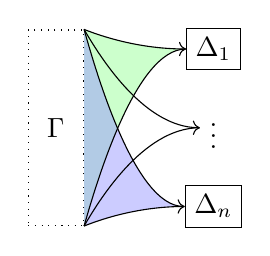
\begin{tikzpicture}[baseline]
    \path
    (-1,1) node (Gtop) {}
    (-1,0) node (G) {$\Gamma$}
    (-1,-1) node (Gbot) {}
    ;
    \node[draw,dotted,fit=(Gtop) (G) (Gbot)] (GG) {};

    \path
    (1,1) node[draw] (Dtop) {$\Delta_1$}
    (1,0) node (D) {$\vdots$}
    (1,-1) node[draw] (Dbot) {$\Delta_n$}
    ;

    \fill[green!20!white,opacity=1] (GG.north east)
    parabola[bend at end] (Dtop.west)
    parabola[bend at start] (GG.south east)
    -- cycle;
    \fill[blue!40!white,opacity=.5] (GG.north east)
    parabola[bend at end] (Dbot.west)
    parabola[bend at start] (GG.south east)
    -- cycle;

    \draw[->] (GG.north east) parabola[bend at end] (Dtop.west);
    \draw (GG.south east) parabola[bend at end] (Dtop.west);
    \draw[->] (GG.north east) parabola[bend at end] (D.west);
    \draw (GG.south east) parabola[bend at end] (D.west);
    \draw[->] (GG.north east) parabola[bend at end] (Dbot.west);
    \draw (GG.south east) parabola[bend at end] (Dbot.west);
  \end{tikzpicture}
\end{displaymath}

To account for usage, we must replace the simple repetition of $\Gamma$ by
repetition of just the types $\gamma$ and \emph{redistribution} of the usage
annotations $\grP$.
Fortunately, our three basic ways of sharing up usage vectors --- zero,
addition, and scaling --- apply directly to the three possible shapes of the
target context --- empty, concatenation, and a usage-annotated singleton.

\begin{definition}[Usage-annotated recursive environment]\label{def:lr-rec-env}
  A \emph{recursive $\V$-environment} between annotated contexts $\Gamma$ and
  $\Delta$ is defined by cases on the shape of $\Delta$ (where
  $\Gamma \env\V_R \Delta$ is the notation for the
  type of recursive environments for given $\V$, $\Gamma$, and $\Delta$):
  \begin{itemize}
    \item There is one environment $\alr{} : \grP\gamma \env\V_R {\cdot}$
      whenever $\grP \leq \gr0$.
    \item For $\rho_l : \grPl\gamma \env\V_R \Delta_l$ and
      $\rho_r : \grPr\gamma \env\V_R \Delta_r$, we have an environment
      $\alr{\rho_l, \rho_r} : \grP\gamma \env\V_R \Delta_l, \Delta_r$ whenever
      $\grP \leq \grPl + \grPr$.
    \item For any value $v : \V\,\grPprime\gamma\,A$, we have an environment
      $\alr{v} : \grP\gamma \env\V_R \gr rA$ whenever
      $\grP \leq \gr r\grPprime$.
  \end{itemize}
\end{definition}

\begin{example}
  Take $\Ann = \plr{\mathbb N, =, 0, +, 1, \times}$, with the equality order
  chosen to avoid any concerns around subsumption of annotations.
  Then, there is an intuitionistic recursive environment as follows, where
  $y\,z$ is the application of $y$ to $z$.
  \[
    \alr{\alr{z},\alr{y\,z}} :
    \plr{x : A, y : B \to C, z : B} \env\vdash_R \plr{B, C}.
  \]
  There is also a usage-aware recursive environment
  \[
    \alr{\alr{z},\alr{y\,z}} :
    \plr{\gr0x : A, \gr2y : B \multimap C, \gr3z : B} \env\vdash_R
    \plr{\gr1B, \gr2C}.
  \]
  The latter relies on the observations that
  $\begin{pmatrix} \gr0 & \gr2 & \gr3 \end{pmatrix} =
  \begin{pmatrix} \gr0 & \gr0 & \gr1 \end{pmatrix}
  + \begin{pmatrix} \gr0 & \gr2 & \gr2 \end{pmatrix}$ and, on the right, that
  $\begin{pmatrix} \gr0 & \gr2 & \gr2 \end{pmatrix} =
  \gr2\begin{pmatrix} \gr0 & \gr1 & \gr1 \end{pmatrix}$.
  Then, we have $\gr0x : A, \gr0y : B \multimap C, \gr1z : B \vdash z : B$ and
  $\gr0x : A, \gr1y : B \multimap C, \gr1z : B \vdash y\,z : C$.
\end{example}

From the example, we can see that the important usage vectors are the initial
one $\begin{pmatrix} \gr0 & \gr2 & \gr3 \end{pmatrix}$ and the usage vectors
at which terms are derived: $\begin{pmatrix} \gr0 & \gr0 & \gr1 \end{pmatrix}$
and $\begin{pmatrix} \gr0 & \gr1 & \gr1 \end{pmatrix}$.
I will call the latter the \emph{leaf vectors}.
The intermediate vector $\begin{pmatrix} \gr0 & \gr2 & \gr2 \end{pmatrix}$ can
be worked out from the leaf vector
$\begin{pmatrix} \gr0 & \gr1 & \gr1 \end{pmatrix}$ and the scaling factor
$\gr2$ found in the codomain context $\gr1B, \gr2C$.
Even when the ordering on annotations is given by a non-equivalence relation
$\leq$, there is a canonical least choice for all of the intermediate vectors,
together with a constraint that the entire linear combination of all the leaf
vectors is less than or equal to the initial usage vector.
In symbols, we may let $\gr\Psi$ be the collection of leaf vectors indexed by
items in $\Delta$, and state
the constraint as $\grP \leq \sum_{\plr{x : \gr rA} \in \Delta} \gr r\gr\Psi_x$.
Seeing $\gr\Psi$ instead as a $\size\Delta \times \size\Gamma$ matrix, this
constraint is $\grP \leq \grQ\gr\Psi$, using vector-matrix multiplication.
The resulting picture is below, showing $\grP$ being split up into $\gr\Psi$,
and then each $\V$-value being constructed in a separate $\gr\Psi_i\gamma$.

\begin{displaymath}
  \begin{tikzpicture}[baseline]
    \path
    (-1,1) node (Gtop) {}
    (-1,0) node (G) {$\grP\gamma$}
    (-1,-1) node (Gbot) {}
    ;
    \node[draw,dotted,fit=(Gtop) (G) (Gbot)] (GG) {};

    \path
    (1,1) node (Dtop) {}
    (1,0) node (D) {$\grQ\delta$}
    (1,-1) node (Dbot) {}
    ;
    \node[draw,dotted,fit=(Dtop) (D) (Dbot)] (DD) {};

    \draw[->,double] (GG) -- (DD);
  \end{tikzpicture}
  \coloneqq
  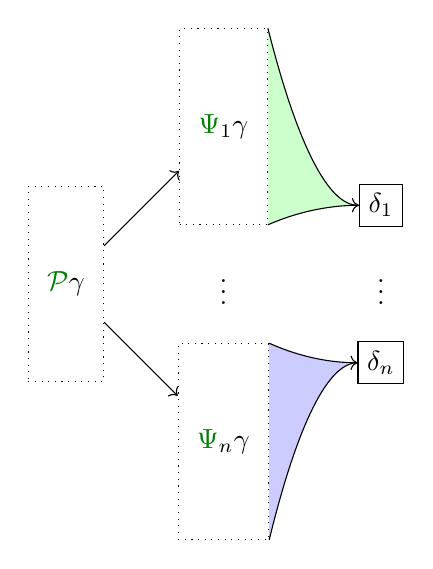
\begin{tikzpicture}[baseline]
    \path
    (-1,1) node (Gtop) {}
    (-1,0) node (G) {$\grP\gamma$}
    (-1,-1) node (Gbot) {}
    ;
    \node[draw,dotted,fit=(Gtop) (G) (Gbot)] (GG) {};

    \path
    (1,3) node (G1top) {}
    (1,2) node (G1) {$\gr\Psi_1\gamma$}
    (1,1) node (G1bot) {}
    ;
    \node[draw,dotted,fit=(G1top) (G1) (G1bot)] (GG1) {};
    \draw[->] (GG) -- (GG1);

    \path (1,0) node {$\vdots$};

    \path
    (1,-1) node (Gntop) {}
    (1,-2) node (Gn) {$\gr\Psi_n\gamma$}
    (1,-3) node (Gnbot) {}
    ;
    \node[draw,dotted,fit=(Gntop) (Gn) (Gnbot)] (GGn) {};
    \draw[->] (GG) -- (GGn);

    \path
    (3,1) node[draw] (Dtop) {$\delta_1$}
    (3,0) node (D) {$\vdots$}
    (3,-1) node[draw] (Dbot) {$\delta_n$}
    ;

    \fill[green!20!white] (GG1.north east)
    parabola[bend at end] (Dtop.west)
    parabola[bend at start] (GG1.south east)
    -- cycle;
    \draw[->] (GG1.north east) parabola[bend at end] (Dtop.west);
    \draw (GG1.south east) parabola[bend at end] (Dtop.west);

    \fill[blue!20!white] (GGn.north east)
    parabola[bend at end] (Dbot.west)
    parabola[bend at start] (GGn.south east)
    -- cycle;
    \draw[->] (GGn.north east) parabola[bend at end] (Dbot.west);
    \draw (GGn.south east) parabola[bend at end] (Dbot.west);
  \end{tikzpicture}
  \quad\textrm{where }\grP \leq \grQ\gr\Psi
\end{displaymath}

From this point, we can recover a functional-style definition of usage-aware
environments.
We choose our leaf vectors $\gr\Psi$ up-front, check the inequality, and then
produce a value at each leaf vector.
%From this definition, we can recover a functional-style definition by
%separating choices of usage vectors from the provision of $\V$-values.
%In particular, the only choices of usage vectors that are essential are the
%$\grPprime$s in the singleton case, with the choices in the concatenation case
%being determined as scalings and sums of these $\grPprime$s.
%I let $\gr\Psi$ collect up these $\size\Delta$-many choices of
%$\size\Gamma$-length usage vectors and note that the constraint on $\gr\Psi$
%generated by all the scaling and summing is
%$\grP = \sum_{\plr{x : \gr rA} \in \Delta} \gr r\gr\Psi_x$.

\begin{definition}[Usage-annotated environment (tentative)]
  A \emph{$\V$-environment} between annotated contexts $\Gamma$ and $\Delta$
  (written $\grP\gamma$ and $\grQ\delta$, respectively, when convenient)
  is a matrix $\gr\Psi : \Ann^{\size\Delta \times \size\Gamma}$ such that
  $\grP \leq \grQ\gr\Psi$ and for each
  $\plr{x : A} \in \delta$ we have a value of type $\V\,\gr\Psi_x\gamma\,A$.
\end{definition}

I find this definition somewhat fiddly because of its reliance on low-level
concepts like non-usage-checked variables and rows of a matrix.
We note that $\gr\Psi_x = \bra x\gr\Psi$, from which point, requiring not
just $\V\,\gr\Psi_x\gamma\,A$ but rather $\V\,\plr{\grQprime\gr\Psi}\gamma\,A$
for any $\grQprime \leq \bra x$ is a minor change (and equivalent if $\V$
respects subusaging, which is practically always the case).
``An $x$ such that $(x : A) \in \delta$ and $\grQprime \leq \bra x\gr\Psi$''
is exactly the definition of $\grQprime\delta \sqni A$.
I further regularise this clause by asking for a
$\grPprime \leq \grQprime\gr\Psi$ rather than $\grQprime\gr\Psi$ exactly,
leaving us needing, for each $\grPprime$ and $\grQprime$ related in the same
way ($\gr\Psi$) as $\grP$ and $\grQ$, a function from $\grQprime\delta \sqni A$
to $\V\,\grPprime\gamma\,A$.
Finally, I choose to switch from matrices and matrix multiplication to
linear maps and their actions, which are easier to work with.
All of these changes yield my primary definition of an environment for
usage-annotated calculi, which will be used for the rest of this chapter and in
\cref{sec:framework}.

\begin{definition}[Usage-annotated environment]\label{def:lr-env}
  A \emph{$\V$-environment} between annotated contexts $\Gamma$ and $\Delta$
  (written $\grP\gamma$ and $\grQ\delta$, respectively, when convenient)
  is a linear map $\gr\Psi : \Ann^{\size\Delta} \to \Ann^{\size\Gamma}$ (written
  postfix) such that $\grP \leq \grQ\gr\Psi$ and for each $A$, $\grPprime$, and
  $\grQprime$ such that $\grPprime \leq \grQprime\gr\Psi$, a function from
  $\grQprime\delta \sqni A$ to $\V\,\grPprime\gamma\,A$.
\end{definition}
\begin{notation}
  When there are multiple environments in question and $\rho$ is such an
  environment, I use the notation $\rho.\gr\Psi$ to refer to $\gr\Psi$.
  For example, $\grP \leq \grQ\plr{\rho.\gr\Psi}$.
  For the action on variables, I write $\rho(x)$, where
  $x : \grQprime\delta \sqni A$.
  The expression ``$\rho(x)$'' alone is ambiguous because of the slack in the
  usage context $\grPprime$ of the resulting value.
  Therefore, I will always make sure $\grPprime$ and $\grQprime$ clear when
  using this notation.
\end{notation}

The following simple lemma shows that usage-annotated environments are, in a
sense, as good as simple environments on usage-checked variables.
What usage-annotated environments give us beyond simple environments is the
ability to accommodate linear decompositions, in a way I will make precise in
the next section.

\begin{lemma}
  We can use an environment $\rho : \Gamma \env\V \Delta$ to map a
  usage-checked variable $x : \Delta \sqni A$ to a value of type
  $\V\,\Gamma\,A$.
\end{lemma}
\begin{proof}
  Let $\Gamma = \grP\gamma$ and $\Delta = \grQ\delta$.
  Set $\grPprime \coloneqq \grP$ and $\grQprime \coloneqq \grQ$, then
  $\grP \leq \grQ\gr\Psi$ by the constraint in $\rho$, so we can take
  the $\V$-value $\rho(x)$.
\end{proof}

\section{Properties of linear environments}\label{sec:lenv}
I settle on \cref{def:lr-env}, and prove various properties about it.

\begin{lemma}\label{thm:env-resize}
  Given an environment $\rho : \grP\gamma \env\V \grQ\delta$ and a $\grPprime$
  and a $\grQprime$ such that $\grPprime \leq \grQprime\plr{\rho.\gr\Psi}$,
  there is also an environment of type $\grPprime\gamma \env\V \grQprime\delta$
  with the same linear map and action on variables.
\end{lemma}
\begin{proof}
  The only part of the definition of an environment dependent on $\grP$ or
  $\grQ$ is the constraint $\grP \leq \grQ\gr\Psi$, which we are able to
  replace for $\grPprime$ and $\grQprime$.
\end{proof}

When constructing an environment, we can do so by cases on the shape of the
target context.
We can create an environment into the empty context when all usage annotations
on the source context are $\gr0$.
We can create an environment into a concatenated context when we can additively
split up the annotations of the source context and produce environments into
both halves from the split sources.
We can create an environment into a singleton context when there is a context
$\gr r$ times smaller than the source context in which we can produce a value
of the appropriate type.

\begin{lemma}\label{thm:construct-env}
  We can define all of the following equivalences for any values of the free
  variables, assuming that $\V$ respects subusaging (i.e.,
  $\grPprime \leq \grP \to
  \V\,\grP\gamma \rightarrowtriangle \V\,\grPprime\gamma$).
  \begin{itemize}
    \item $I^{\sep} \leftrightarrowtriangle \plr{{-} \env\V {\cdot}}$
    \item $\plr{{-} \env\V \Delta_l} \sep \plr{{-} \env\V \Delta_r}
      \leftrightarrowtriangle \plr{{-} \env\V \Delta_l, \Delta_r}$
    \item $\gr r \cdot \plr{\V\,(-)\,A}
      \leftrightarrowtriangle \plr{{-} \env\V \gr rA}$
  \end{itemize}
\end{lemma}
\begin{proof}
  There are 6 cases to check.
  Throughout, we write $\Gamma$ as $\grP\gamma$ and $\Delta$ as $\grQ\delta$
  when convenient.
  \begin{description}
    \item[$I^{\sep}(\rightarrowtriangle)$]
      Let $\gr\Psi$ be the unique linear map out of the zero space.
      By assumption and definition, $\grP \leq \gr0 = \grQ\gr\Psi$.
      There are no variables to act upon.
    \item[$I^{\sep}(\leftarrowtriangle)$]
      $\grQ\gr\Psi$ is an empty sum, so if $\grP \leq \grQ\gr\Psi$ then
      $\grP \leq \gr0$.
    \item[$\sep(\rightarrowtriangle)$]
      Let the given environments be $\rho_l : \grPl\gamma \env\V \grQl\delta$
      and $\rho_r : \grPr\gamma \env\V \grQr\delta$, with
      $\grP \leq \grPl + \grPr$.
      Define $\gr\Psi \coloneqq [\rho_l.\gr\Psi, \rho_r.\gr\Psi]$, using the
      coproduct structure of the concatenated vector space.
      We have $\grP \leq \grPl + \grPr \leq
      \grQl\plr{\rho_l.\gr\Psi} + \grQr\plr{\rho_r.\gr\Psi} =
      \begin{pmatrix} \grQl & \grQr \end{pmatrix}\gr\Psi$.
      To act on variables, we are given $\grPprime \leq
      \begin{pmatrix} \gr{\grQ'_l} & \gr{\grQ'_r} \end{pmatrix}\gr\Psi$ and
      $\gr{\grQ'_l}\delta_l, \gr{\grQ'_r}\delta_r \sqni A$.
      Without loss of generality, let us have $\gr{\grQ'_l}\delta_l \sqni A$
      and $\gr{\grQ'_r} \leq \gr0$.
      Thus, $\grPprime \leq
      \gr{\grQ'_l}\plr{\rho_l.\gr\Psi} + \gr{\grQ'_r}\plr{\rho_r.\gr\Psi} \leq
      \gr{\grQ'_l}\plr{\rho_l.\gr\Psi}$,
      and we can act on the variable using $\rho_l$.
    \item[$\sep(\leftarrowtriangle)$]
      Let the unnamed context be $\Gamma$, also written $\grP\gamma$.
      The linear map
      $\gr\Psi : \Ann^{\size{\Delta_l} + \size{\Delta_r}} \to \Ann^{\size\Gamma}$
      splits into
      $\gr\Psi_{\gr l} : \Ann^{\size{\Delta_l}} \to \Ann^{\size\Gamma}
      \coloneqq \alr{\id, 0}; \gr\Psi$ and
      $\gr\Psi_{\gr r} : \Ann^{\size{\Delta_r}} \to \Ann^{\size\Gamma}
      \coloneqq \alr{0, \id}; \gr\Psi$, using the product structure of
      the concatenated vector space.
      Let $\grPl \coloneqq \grQl\gr\Psi_{\gr l}$ and
      $\grPr \coloneqq \grQr\gr\Psi_{\gr r}$, by definition satisfying the
      required constraints.
      For the action on variables, let us consider the left environment (with
      the right environment following symmetrically).
      We are given $\gr{\grP'_l} \leq \gr{\grQ'_l}\gr\Psi_{\gr l}$ and
      $\gr{\grQ'_l}\delta_l \sqni A$.
      From these, we get
      $\gr{\grP'_l} \leq \gr{\grQ'_l}\gr\Psi_{\gr l} =
      \begin{pmatrix} \gr{\grQ'_l} & \gr0 \end{pmatrix}\gr\Psi$ and
      $\gr{\grQ'_l}\delta_l, \gr0\delta_r \sqni A$.
      We can therefore act using the original environment.
    \item[$\cdot(\rightarrowtriangle)$]
      Let $\grP$ and $\grPprime$ be such that $\grP \leq \gr r\grPprime$ and let
      $v : \V\,\grPprime\gamma\,A$.
      Let $\gr\Psi : \Ann \to \Ann^{\size\gamma}
      \coloneqq \gr r\gr' \mapsto \gr r\gr'\grPprime$.
      By definition and the previous assumption, we have
      $\grP \leq \gr r\gr\Psi$.
      When acting on a variable, we have $\grP\gr{''} \leq \gr r\gr'\gr\Psi$
      and $\gr r\gr'A \sqni A'$.
      The latter tells us that $A = A'$ and $\gr r\gr' \leq \gr1$.
      Thus, $\grP\gr{''} \leq \grPprime$.
      Therefore, by subusaging, we may produce a value of type
      $\V\,\grPprime\gamma\,A$, which we can take to be $v$.
    \item[$\cdot(\leftarrowtriangle)$]
      Let us have an environment of type $\grP\gamma \env\V \gr rA$.
      We want to use its action on variables to yield a value.
      To do this, we let $\grPprime \coloneqq \gr1\gr\Psi$, and use this
      equation, together with the fact that we have a variable of type
      $\gr1A \sqni A$, to get a value of type $\V\,\grPprime\gamma\,A$.
      Furthermore, we derive $\grP \leq \gr r\gr\Psi = \gr r\grPprime$, as
      required.
  \end{description}
\end{proof}

We could, as in \cref{def:lr-rec-env}, use these three clauses to define what an
environment is.
However, such a definition appears to require creative induction hypotheses in
the proving of simple lemmas, in contrast to the more direct proofs I achieve
below using \cref{def:lr-env}.
To take a concrete example, consider how we may construct an ``identity''
environment of type $\Gamma \env\V \Gamma$, as in \cref{thm:env-id} below.
If we try to directly proceed by induction on $\Gamma$, we get to the case where
we are aiming to construct an environment of type
$\grP\gamma, \grQ\delta \env\V \grP\gamma, \grQ\delta$ by constructing
environments of types $\grP\gamma, \gr0\delta \env\V \grP\gamma$ and
$\gr0\gamma, \grQ\delta \env\V \grQ\delta$.
These are not identity environments, and thus do not come from the hypotheses of
a simple induction.
In contrast, using \cref{def:lr-env}, in \cref{thm:env-id} we are able to use
the standard fact that there are identity linear maps, and on top of such a map
worry only about the value assigned to each variable.

One of the primary test cases for environments is simultaneous substitution,
which will look like the \TirName{sub} rule below.
Note that we have taken $\V \coloneqq {\vdash}$ --- i.e.\ that the values
yielded by the environment are terms, namely the terms to be substituted in for
the free variables of the derivation of $\Delta \vdash A$.

\begin{displaymath}
  \begin{prooftree}
    \hypo{\Gamma \env{\vdash} \Delta}
    \hypo{\Delta \vdash A}
    \infer2[sub]{\Gamma \vdash A}
  \end{prooftree}
\end{displaymath}

The admissibility of substitution will be by induction on the derivation of
$\Delta \vdash A$, so we will need to be able to adapt any environment we are
given to work with any possible context of new premises yielded by the rules of
\cref{fig:lr-bunched}.
In the simply typed case, the only change to the context we encountered was the
binding of new variables.
With usage annotations, we furthermore have linear decompositions of the
context, necessitating changes to the environment whenever usage annotations
change.

There are three kinds of linear decompositions we have to deal with: zero,
addition, and scaling; corresponding to bunched connectives $I^*$, $\sep$, and
$\gr r \cdot {}$, respectively.
In each of these three cases, we have a simple preservation lemma, transforming
an environment
of type $\Gamma \env\V \Delta$ and a decomposition of $\Delta$ into a
decomposition of $\Gamma$ and environments for all of the decomposed fragments
of $\Gamma$ and $\Delta$.

\begin{lemma}[environments preserve zero]\label{thm:lr-env-zero}
  Given an environment $\rho : \grP\gamma \env\V \grQ\delta$ such that
  $\grQ \leq \gr 0$, we also have that $\grP \leq \gr 0$.
\end{lemma}
\begin{proof}
  $\grP \leq \grQ\gr\Psi \leq \gr0\gr\Psi = \gr0$, by environment
  compatibility from $\rho$ and monotonicity and linearity of $\gr\Psi$.
\end{proof}

\begin{lemma}[environments preserve addition]\label{thm:lr-env-add}
  Given an environment $\rho : \grP\gamma \env\V \grQ\delta$ such that
  $\grQ \leq \grQl + \grQr$ for some $\grQl$ and $\grQr$, we also have $\grPl$
  and $\grPr$ such that $\grP \leq \grPl + \grPr$ and there are environments
  $\rho_l : \grPl\gamma \env\V \grQl\delta$ and
  $\rho_r : \grPr\gamma \env\V \grQr\delta$.
\end{lemma}
\begin{proof}
  Let $\grPl \coloneqq \grQl\gr\Psi$ and $\grPr \coloneqq \grQr\gr\Psi$.
  Then, $\grP \leq \grQ\gr\Psi \leq \plr{\grQl + \grQr}\gr\Psi =
  \grQl\gr\Psi + \grQr\gr\Psi = \grPl + \grPr$, satisfying the first condition.
  Because clearly $\grPl \leq \grQl\gr\Psi$ and $\grPr \leq \grQr\gr\Psi$,
  applying \cref{thm:env-resize} to $\rho$ gives us the required
  new environments $\rho_l$ and $\rho_r$.
\end{proof}

\begin{lemma}[environments preserve scaling]\label{thm:lr-env-scale}
  Given an environment $\rho : \grP\gamma \env\V \grQ\delta$ such that
  $\grQ \leq \gr r\grQprime$ for some $\grQprime$, we also have a $\grPprime$
  such that $\grP \leq \gr r\grPprime$ and there is an environment
  $\rho' : \grPprime\gamma \env\V \grQprime\delta$.
\end{lemma}
\begin{proof}
  Let $\grPprime \coloneqq \grQprime\gr\Psi$.
  Then, $\grP \leq \grQ\gr\Psi \leq \plr{\gr r\grQprime}\gr\Psi =
  \gr r\plr{\grQprime\gr\Psi} = \gr r\grPprime$, satisfying the first condition.
  Because clearly $\grPprime \leq \grQprime\gr\Psi$,
  applying \cref{thm:env-resize} to $\rho$ gives us the required
  new environment $\rho'$.
\end{proof}

The final change environments need to preserve is the binding of new free
variables.
In \cref{sec:syntactic-kits}, we had the operation \AgdaFunction{bindEnv} for
this purpose in the intuitionistic setting.
There, we relied on $\V$ supporting a map from $\ni$-variables and admitting
weakening.
In the usage-annotated setting, the former requirement is updated to having a
map from usage-checked $\sqni$-variables.
As for the latter requirement, it turns out that we only need $\V$ to admit
weakening by $\gr0$-annotated variables, which is much more reasonable than
general weakening.
\Cref{thm:lr-bind} adapts \AgdaFunction{bindEnv} for the usage-annotated
setting.

\begin{lemma}[\AgdaFunction{bindEnv}]\label{thm:lr-bind}
  Given functions
  ${\swarrow^k} : \forall \Gamma, \grR, \theta.~\grR \leq \gr0 \to
  \V\,\Gamma \rightarrowtriangle \V\,\plr{\Gamma, \grR\theta}$ and
  $\mathrm{vr} : {\sqni} \rightarrowtriangle \V$, we can turn an environment of
  type $\Gamma \env\V \Delta$ into an environment of type
  $\Gamma, \Theta \env\V \Delta, \Theta$ for any context $\Theta$.
\end{lemma}
\begin{proof}
  Let $\grP\gamma \coloneqq \Gamma$, $\grQ\delta \coloneqq \Delta$, and
  $\grR\theta \coloneqq \Theta$.
  Let the new linear map $\gr\Psi\gr' : \Ann^{\size\Delta + \size\Theta} \to
  \Ann^{\size\Gamma + \size\Theta}$ be $\gr\Psi \oplus \gr I$.
  That is, in block matrix notation,
  $\begin{pmatrix} \gr\Psi & \gr0 \\ \gr0 & \gr I \end{pmatrix}$.
  Checking that this linear map fits, we have
  $\begin{pmatrix}\grP & \grR\end{pmatrix}
  \leq \begin{pmatrix}\grQ\gr\Psi & \grR\gr I\end{pmatrix}
  = \begin{pmatrix}\grQ & \grR\end{pmatrix}\plr{\gr\Psi \oplus \gr I}$.
  For the action on variables, we are given vectors $\grPprime$,
  $\grR\gr'_\grP$, $\grQprime$, and $\grR\gr'_\grQ$ such that
  $\begin{pmatrix} \grPprime & \grR\gr'_\grP \end{pmatrix} \leq
  \begin{pmatrix} \grQprime & \grR\gr'_\grQ \end{pmatrix}
  \plr{\gr\Psi \oplus \gr I}$ and we have a variable of type
  $\grQprime\delta, \grR\gr'_\grQ\theta \sqni A$ for some type $A$.
  The constraint on the new vectors reduces to $\grPprime \leq \grQprime\gr\Psi$
  and $\grR\gr'_\grP \leq \grR\gr'_\grQ$.
  From the variable we either have a variable $x$ in $\delta$ with
  $\grQprime \leq \langle x \rvert$ and $\grR\gr'_\grQ \leq \gr0$, or a
  variable $y$ in $\theta$ with $\grQprime \leq \gr0$ and
  $\grR\gr'_\grQ \leq \langle y \rvert$.
  In the former case, the action of the original environment on $x$ gives us a
  $\V$-value in $\grPprime\gamma$, and the $\gr0$-weakening principle
  $\swarrow^k$, noting that $\grR\gr'_\grP \leq \grR\gr'_\grQ \leq \gr0$, gives
  us a $\V$-value in $\grPprime\gamma, \grR\gr'_\grP\theta$.
  In the latter case, we have that
  $\begin{pmatrix} \grPprime & \grR\gr'_\grP \end{pmatrix}
  \leq \begin{pmatrix} \grQprime\gr\Psi & \grR\gr'_\grQ \end{pmatrix}
  \leq \begin{pmatrix} \gr0\gr\Psi & \langle y \rvert \end{pmatrix}
  = \begin{pmatrix} \gr0 & \langle y \rvert \end{pmatrix}
  = \left\langle {\searrow}y \right\rvert$, so $y$ also serves as a
  usage-checked variable in $\grPprime\gamma, \grR\gr'_\grP\theta$.
  From this usage-checked variable, we get a $\V$-value in the same context
  using $\mathrm{vr}$.
\end{proof}

I put together the preceding pieces to give a syntactic traversal operation over
$\name$ in the following section.
For the rest of this section, I observe some more constructions purely on
environments --- in particular, composition of environments given certain
assumptions about the families of values.

Following \citet{ACU15}, we expect (intuitionistic) ST$\lambda$C syntax to form
a relative monad over $\ni$ seen as a functor from the category of contexts
under renaming to the functor category $\blr{\mathrm{Ty}, \Set}$, where
$\mathrm{Ty}$ is the discrete category of ST$\lambda$C types.
Notice that, given $F,G : \blr{\mathrm{Ty}, \Set}$, a morphism from $F$ to $G$
is a function of type $F \rightarrowtriangle G$ (with naturality being trivial).
Therefore, we expect a relative monad, given as a Kleisli triple, to have a unit
$\eta_\Gamma : \Gamma \ni \plr{-} \rightarrowtriangle \Gamma \vdash \plr{-}$
given by the variable rule, and a Kleisli extension operator
${^*}_{\Gamma,\Delta} :
\plr{\Gamma \ni \plr{-} \rightarrowtriangle \Delta \vdash \plr{-}} \to
\plr{\Gamma \vdash \plr{-} \rightarrowtriangle \Delta \vdash \plr{-}}$
given by substitution.
Composition of substitutions falls out of this framework as Kleisli composition.
However, in the usage-aware case, substitution needs not just a mapping of
variables $f : \Gamma \sqni \plr{-} \rightarrowtriangle \Delta \vdash \plr{-}$,
but rather an environment $\rho : \Delta \env\vdash \Gamma$, as we have already
discussed.
It therefore makes sense for our replacement for the Kleisli extension operator
to similarly take an environment rather than a simple variable mapping.

\Cref{thm:env-comp} below amounts to deriving a modified notion of Kleisli
composition from a modified Kleisli extension.
Additionally, \cref{thm:env-id} is required to turn a monadic unit into an
identity environment.
Both lemmas are stated in terms of general $\U$/$\V$/$\W$-environments, with
some specific examples (e.g.\ for renaming and substitution) below them.

\begin{lemma}[Identity environment]\label{thm:env-id}
  Given a function
  \[
    \mathrm{vr}_{\Gamma'} :
    \Gamma' \sqni \plr{-} \rightarrowtriangle \V\,\Gamma'
  \]
  for any
  $\Gamma$ we have an environment $\mathrm{id} : \Gamma \env\V \Gamma$.
\end{lemma}
\begin{proof}
  Let $\Gamma = \grP\gamma$.
  Let $\gr\Psi$ be the identity map, which clearly satisfies
  $\grP \leq \grP\gr\Psi$.
  When acting on a variable, the inequality $\grPprime \leq \grQprime\gr\Psi$
  means that $\grPprime \leq \grQprime$.
  We are given a variable of type $\grQprime\gamma \sqni A$, which we can
  coerce to a variable of type $\grPprime\gamma \sqni A$, upon which we apply
  $\mathrm{vr}$ to get the required value of type $\V\,\grPprime\gamma\,A$.
\end{proof}

\begin{lemma}[Composition of environments]\label{thm:env-comp}
  Given a function
  \[
    \mathrm{lift}_{\Gamma', \Delta'} :
    \Gamma' \env\U \Delta' \to \V\,\Delta' \rightarrowtriangle \W\,\Gamma'
  \]
  we can compose environments $\rho : \Gamma \env\U \Delta$ and
  $\sigma : \Delta \env\V \Theta$ into an environment
  $\rho \gg \sigma : \Gamma \env\W \Theta$.
\end{lemma}
\begin{proof}
  Let $\Gamma = \grP\gamma$, $\Delta = \grQ\delta$, and $\Theta = \grR\theta$.
  Take $\gr\Psi$ to be the composition $\plr{\sigma.\gr\Psi}\plr{\rho.\gr\Psi}$,
  noting that
  $\grP \leq \grQ\plr{\rho.\gr\Psi} \leq
  (\grR\plr{\sigma.\gr\Psi})\plr{\rho.\gr\Psi} = \grR\gr\Psi$
  thanks to the inequalities yielded by $\sigma$ and $\rho$.
  When acting on a variable, we are given $\grPprime \leq \grRprime\gr\Psi$ and
  a variable $v : \grRprime\theta \sqni A$, and want a value of type
  $\W\,\grPprime\gamma\,A$.
  Let $\grQprime \coloneqq \grRprime\plr{\sigma.\gr\Psi}$, with inequality
  $\grQprime \leq \grRprime\plr{\sigma.\gr\Psi}$ giving us a value
  $\sigma(v) : \V\,\grQprime\delta\,A$.
  We wish to apply $\mathrm{lift}$ to $\sigma(v)$ with
  $\Gamma' \coloneqq \grPprime\gamma$ and $\Delta' \coloneqq \grQprime\delta$ to
  complete the construction of the $\W$-value.
  To do this, we need an environment of type
  $\grPprime\gamma \env\U \grQprime\delta$, which we can get from $\rho$ using
  \cref{thm:env-resize}, noting that
  $\grPprime \leq \grRprime\plr{\sigma.\gr\Psi}\plr{\rho.\gr\Psi} =
  \grQprime\plr{\rho.\gr\Psi}$.
\end{proof}

We can derive the following corollaries as instances of environment composition.

\begin{corollary}[Composition of renamings]\label{thm:ren-comp}
  Given renamings $\rho : \Gamma \env\sqni \Delta$ and
  $\sigma : \Delta \env\sqni \Theta$, we can form their composite
  $\rho; \sigma : \Gamma \env\sqni \Theta$.
\end{corollary}
\begin{proof}
  Take $\U = \V = \W = {\sqni}$ in \cref{thm:env-comp}.
  Then let $\mathrm{lift}\,\rho\,x \coloneqq \rho(x)$.
\end{proof}

\begin{corollary}[Post-composition with a renaming]\label{thm:ren-env-comp}
  Given an environment $\rho : \Gamma \env\U \Delta$ and a renaming
  $\sigma : \Delta \env\sqni \Theta$, we can form their composite
  $\rho; \sigma : \Gamma \env\U \Theta$.
\end{corollary}
\begin{proof}
  As in \cref{thm:ren-comp}.
\end{proof}

\begin{corollary}[Pointwise renaming of an environment]\label{thm:env-ren}
  If $\sdtstile{}\V$ respects renaming, then so does $\env\V$ (on the left).
\end{corollary}
\begin{proof}
  Suppose we have $\rho : \Gamma \env\sqni \Delta$ and
  $\sigma : \Delta \env\V \Theta$.
  We want to compose these via \cref{thm:env-comp} with $U = {\sqni}$ and
  $\V = \W$.
  The function $\mathrm{lift}$ is given exactly by the fact that $\V$ respects
  renaming.
\end{proof}

\begin{corollary}[Composition of substitutions]\label{thm:sub-comp}
  Given substitutions $\rho : \Gamma \env\vdash \Delta$ and
  $\sigma : \Delta \env\vdash \Theta$, we can form their composite
  $\rho; \sigma : \Gamma \env\vdash \Theta$.
\end{corollary}
\begin{proof}
  Take $\U = \V = \W = {\vdash}$ in \cref{thm:env-comp}.
  Then, $\mathrm{lift}$ is given by the action of a substitution on a term
  (see \AgdaFunction{sub} in the following section).
\end{proof}

\begin{corollary}[Composing semantics with substitution]
  If we have a semantics (in the sense of \cref{sec:gen-sem} and
  \cref{sec:traversal}) from $\U$ to $\W$, then from an environment
  $\rho : \Gamma \env\U \Delta$ and a substitution
  $\sigma : \Delta \env\vdash \Theta$, we can form the composite
  $\rho; \sigma : \Gamma \env\W \Theta$.
\end{corollary}

% Concatenation is difficult; save to after I've talked about renamings.

% Finally for this section, we give the conditions under which the
% context-forming operations (empty, concatenation, and singleton) have a
% functorial action with respect to $\V$-environments.
%
% \begin{lemma}
%   For any $\V$, there is an environment ${\cdot} \env\V {\cdot}$.
% \end{lemma}
% \begin{proof}
%   By \cref{thm:construct-env}, it suffices to show $I\,{\cdot}$, which is
%   trivially true.
% \end{proof}

\section{Substitution is admissible in \name{}}\label{sec:lrsub}
\def\LRKits{../agda/processed-latex/LRKits.tex}

I now show that, using the notion of \emph{environment} derived in
\cref{sec:lrkits}, we can replicate the Agda proofs from
\cref{sec:syntactic-kits} in the usage-aware setting of $\name$.
From \cref{sec:lenv}, we know that environments are preserved under all
syntax-forming operations: zero, addition, scaling, and binding.
What is left is to show how these properties are deployed, and also how to
go on and prove the admissibility of simultaneous renaming, simultaneous
substitution, and then single substitution.

There are a few notational changes necessary in the Agda code, compared to the
typeset mathematics above.
Usage vectors, elsewhere called $\grP$, $\grQ$, and $\grR$ are rendered as
\AgdaBound{P}, \AgdaBound{Q}, and \AgdaBound{R}, respectively.
Usage contexts and typing contexts are tied together with the
\AgdaInductiveConstructor{ctx} constructor, rather than simple juxtaposition.
Environments, elsewhere notated $\Gamma \env\V \Delta$, are rendered as
\AgdaRecord{[}\AgdaSpace{}\AgdaBound{$\V$}\AgdaSpace{}\AgdaRecord{]}%
\AgdaSpace{}\AgdaBound{$\Gamma$}\AgdaSpace{}\AgdaRecord{$\Rightarrow^e$}%
\AgdaSpace{}\AgdaBound{$\Delta$}.

I start with the definition \AgdaFunction{Weakening}, which says what it means
for a family of values \AgdaBound{$\V$} to respect one step of weakening on the
right by $\gr0$-use variables.
I state weakening in a slightly different way to what appears in the statement
of \cref{thm:lr-bind}, so as to help
unification against a known result type (avoiding the problem described by
\citet{McBride12} as \emph{green slime}).
The type \AgdaFunction{Weakening}\AgdaSpace{}\AgdaBound{$\V$} can be read as
saying that, for any context $\grP\gamma$ of shape $s + t$, if the right of
$\grP$ is below $\gr0$, then a value in the left part of $\grP\gamma$ weakens
to a value in the whole of $\grP\gamma$.

\ExecuteMetaData[\LRKits]{Weakening}

Given this new definition of \AgdaFunction{Weakening}, the record
\AgdaRecord{Kit} remains largely unchanged relative to what we saw in
\cref{sec:syntactic-kits}.
We still want $\V$-values to respect weakening (as used in \cref{thm:lr-bind}),
and to support maps \AgdaField{vr} from variables (also used in
\cref{thm:lr-bind}) and \AgdaField{tm} into terms (used when traversal reaches a
variable, we get a value from the environment, and want to produce a term from
that value).
As well as \AgdaFunction{Weakening}, note that \AgdaRecord{\_$\sqni$\_} and, of
course, \AgdaDatatype{\_$\vdash$\_} have different definitions to the
corresponding intuitionistic notions, but they still represent morally the same
parts of the language and its metatheory.

\ExecuteMetaData[\LRKits]{Kit}

To demonstrate the important points succinctly, I cut \name{} down to just the
$\oc\gr r$-fragment.
The introduction rule and pattern-matching eliminator feature scaling, addition,
and variable binding, missing out only on sharing (which is trivial) and zero
(which is simpler than, and analogous to, addition).
The resulting type of well typed terms is below.

\ExecuteMetaData[\LRKits]{Tm}

Given a \AgdaRecord{Kit}\AgdaSpace{}\AgdaBound{$\V$},
\cref{thm:lr-bind} gives a function with the following type.

\ExecuteMetaData[\LRKits]{bindEnv}

Given \AgdaFunction{bindEnv} (\cref{thm:lr-bind}), \AgdaFunction{env-+}
(\cref{thm:lr-env-add}), and \AgdaFunction{env-*} (\cref{thm:lr-env-scale}),
we can reproduce the syntactic traversal \AgdaFunction{trav}.
Similarly to the unchanged high-level definition of \AgdaRecord{Kit}, we are
aiming for an unchanged traversal principle expressed by the rule below.
When $\V$ has a \AgdaRecord{Kit} structure, and we have a $\V$-environment from
$\Gamma$ to $\Delta$, we can transform a term in $\Delta$ to a term in $\Gamma$
of the same type.

\[
  \begin{prooftree}
    \hypo{\text{\AgdaRecord{Kit}\AgdaSpace{}}\V}
    \hypo{\Gamma \env\V \Delta}
    \hypo{\Delta \vdash A}
    \infer3[Trav]{\Gamma \vdash A}
  \end{prooftree}
\]

With all the lemmas of \cref{sec:lenv} in place, writing \AgdaFunction{trav}
becomes routine.
When processing a rule, we work our way up through the
premise connectives, applying \AgdaFunction{env-*} wherever we see a
\AgdaFunction{$\cdot^c$}, \AgdaFunction{env-+} wherever we see a
\AgdaFunction{$*^c$}, and \AgdaFunction{bindEnv} wherever we see a
\AgdaFunction{Bind}.
We then use whatever environments (with names beginning with
\AgdaBound{$\rho$}) and whatever usage vector splitting facts (with names
beginning with \AgdaBound{sp}) come out of this process to recursively
traverse the subterms and recombine the results.

\ExecuteMetaData[\LRKits]{trav}

Instantiating the generic syntactic traversal \AgdaFunction{trav} to renaming
looks just like it did in the intuitionistic case.
I have consistently replaced intuitionistic variables by linear variables, so
\AgdaFunction{id} and \AgdaInductiveConstructor{var} still work to embed
variables into variables and terms, respectively.
Weakening for variables \AgdaFunction{$\swarrow^v$} (not pictured) has been
updated to note that, for $\grP \leq \bra x$ and $\grR \leq \gr0$, we also have
$\begin{pmatrix} \grP & \grR \end{pmatrix} \leq \bra{{\swarrow}x}$.

\ExecuteMetaData[\LRKits]{var-kit}

In the intuitionistic case, environments were just functions, so we passed the
variable weakening function \AgdaFunction{$\swarrow^v$} to the function
\AgdaFunction{ren} to yield a term weakening function.
However, a usage-aware environment is a function packed together with usage
distribution data.
As such, we must make an environment version of \AgdaFunction{$\swarrow^v$}.
I start with a general lemma \AgdaFunction{$\swarrow$\^{}Env}, stating that if
$\V$ supports weakening, then so do $\V$-environments (in their domain
context).
This lemma then specialises to variables, with the identity renaming
\AgdaFunction{id\^{}Env} on the left part of the context and the proof
\AgdaBound{R0} that the right part of the context is below $\gr0$ combining
to give the desired weakening environment.

\ExecuteMetaData[\LRKits]{dlv-env}

This is what we need to instantiate \AgdaFunction{trav} for substitution.
As a reminder, I also give the type of \AgdaFunction{sub} in rule form.

\ExecuteMetaData[\LRKits]{sub}
\[
  \ebrule{%
    \hypo{\Gamma \env\vdash \Delta}
    \hypo{\Delta \vdash B}
    \infer2[sub]{\Gamma \vdash B}
  }
\]

Finally, the simultaneous substitution \AgdaFunction{sub} specialises to
single substitution.

\begin{corollary}[Single substitution]\label{thm:single-sub}
  The following equivalent rules are admissible.
  \begin{mathpar}
    \ebrule{%
      \hypo{\grR \leq \gr r\grP + \grQ}
      \hypo{\grP\gamma \vdash A}
      \hypo{\grQ\gamma, \gr rA \vdash B}
      \infer3{\grR\gamma \vdash B}
    }
    \and
    \ebrule[comb]{%
      \hypo{\gr r \cdot \plr{{} \vdash A}}
      \hypo{\sep}
      \hypo{\gr rA \vdash B}
      \infer3{{} \vdash B}
    }
  \end{mathpar}
\end{corollary}
\begin{proof}
  It is enough to construct a substitution of type
  $\grR\gamma \env\vdash \grQ\gamma, \gr rA$.
  To do this, we use \cref{thm:construct-env} cases $\sep(\rightarrowtriangle)$
  and $\cdot(\rightarrowtriangle)$ on inequalities
  $\grR \leq \grQ + \gr r\grP$ and $\gr r\grP \leq \gr r\grP$ respectively to
  leave us needing a substitution of type $\grQ\gamma \env\vdash \grQ\gamma$ and
  a term of type $\grP\gamma \vdash A$.
  For the substitution, we give the identity substitution (\cref{thm:env-id}),
  and we have the term as a hypothesis.
\end{proof}

\section{Adding recursion to \name{}}\label{sec:rec}
Based on an intuitive understanding of ``usage'', recursion introduces a new
phenomenon relative to the forms of programs we have seen so far:
terms can be used an unbounded number of times.
For example, notice the following reduction in Agda.

\missingfigure{\texttt{foldr \_+\_ 0 (1 :: 2 :: 3 :: []) = 1 + (2 + (3 + 0))}}

The function \AgdaFunction{\_+\_} has been copied into 3 different places in
the running of the program.
This copying is despite no type telling us that \AgdaFunction{\_+\_} would be
used 3 times (both \verb|[1,2,3]| and \verb|[2,3]| have type
\AgdaDatatype{List}\AgdaSpace{}\AgdaDatatype{$\mathbb N$}, despite the
corresponding folds using \AgdaFunction{\_+\_} a different number of times).
As such, when checking an application of \AgdaFunction{foldr}, we need check
that we can use its functional argument (\AgdaFunction{\_+\_} in this case) an
arbitrary number of times.
If we were to fix $\Ann$ as the $\{\gr0, \gr1, \gr\omega\}$ posemiring, then
wrapping the type of the functional argument in $\oc\gr\omega$ would suffice.
However, we want to remain generic in the choice of semiring.

I propose the following additions to \name{} to support a broad class of
inductive types.
I define strictly positive functors syntactically, with the only notable
restriction being not being allowed to use the type variable $X$ in the domain
of a function type.
I then add least fixed points of such strictly positive functors to the syntax
of types.

\begin{align*}
  U &\Coloneqq A \multimap (-) \mid \oc\gr r(-) \\
  {\odot} &\Coloneqq {\otimes} \mid {\oplus} \mid {\with} \\
  F[X], G[X] &\Coloneqq X \mid A \mid U(F[X]) \mid F[X] \odot G[X] \\
  A &\Coloneqq \cdots \mid \mu X.~F[X]
\end{align*}

\begin{example}
  We may define $\mathrm{List}_A \coloneqq \mu X.~I \oplus \plr{A \otimes X}$.
\end{example}

In the typing rules, introduction of an inductive type is standard.
For the elimination rule, we follow a similar pattern to other pattern-matching
rules --- $\oplus$-E, $\otimes$-E, and $\oc$-E --- by splitting the context
and typing the eliminand in one half ($\grP$).
We type the continuation in the other half, but because the continuation may
be used multiple times, and in a modal context, we require that $\grQ$ is
preserved by all linear operations.

\begin{displaymath}
  \begin{prooftree}
    \hypo{\grR\gamma \vdash F[\mu X.~F[X]]}
    \infer1[$\mu$-I]{\grR\gamma \vdash \mu X.~F[X]}
  \end{prooftree}
\end{displaymath}
\begin{displaymath}
  \begin{prooftree}
    \hypo{\grR \leq \grP + \grQ}
    \hypo{\grP\gamma \vdash \mu X.~F[X]}
    \hypo{%
      \begin{matrix*}[l]
        \grQ \leq \gr0 \\
        \grQ \leq \grQ + \grQ \\
        \forall \gr r.~\grQ \leq \gr r\grQ
      \end{matrix*}%
    }
    \hypo{\grQ\gamma, \gr1F[C] \vdash C}
    \infer4[$\mu$-E]{\grR\gamma \vdash C}
  \end{prooftree}
\end{displaymath}

\begin{example}\label{thm:list-rules}
  For lists, we can derive the following introduction and elimination rules
  (with usage constraints omitted for brevity when obvious).

  \begin{align*}
    \begin{prooftree}
      \hypo{\grR \leq \gr0}
      \infer1[$I$-I]{I}
      \infer1[$\oplus$-I$_0$]%
      {\grR\gamma \vdash I \oplus \plr{A \otimes \mathrm{List}_A}}
      \infer1[$\mu$-I]{\grR\gamma \vdash \mathrm{List}_A}
    \end{prooftree}
    &&
    \begin{prooftree}
      \hypo{\grR \leq \grP + \grQ}
      \hypo{\grP\gamma \vdash A}
      \hypo{\grQ\gamma \vdash \mathrm{List}_A}
      \infer3[$\otimes$-I]{\grR\gamma \vdash A \otimes \mathrm{List}_A}
      \infer1[$\oplus$-I$_1$]%
      {\grR\gamma \vdash I \oplus \plr{A \otimes \mathrm{List}_A}}
      \infer1[$\mu$-I]{\grR\gamma \vdash \mathrm{List}_A}
    \end{prooftree}
  \end{align*}
  \begin{displaymath}
    \begin{prooftree}
      \hypo{\grP\gamma \vdash \mathrm{List}_A}
      \infer0[Var]{\gr0\gamma, \gr1\plr{I \oplus \plr{A \otimes C}}
        \vdash I \oplus \plr{A \otimes C}}
      \hypo{\nabla^n}
      \hypo{\nabla^c}
      \infer3[$\oplus$-E]{\grQ\gamma, \gr1\plr{I \oplus \plr{A \otimes C}}
        \vdash C}
      \infer2[$\mu$-E]{\grR\gamma \vdash C}
    \end{prooftree}
  \end{displaymath}
  \begin{align*}
    \textrm{where }\nabla^n &\coloneqq
    \begin{prooftree}
      \infer0[Var]{\gr0\gamma, \gr1I \vdash I}
      \hypo{\grQ\gamma \vdash C}
      \infer1[Wk]{\grQ\gamma, \gr0I \vdash C}
      \infer2[$I$-E]{\grQ\gamma, \gr1I \vdash C}
      \infer1[Wk]{\grQ\gamma, \gr0\plr{I \oplus \plr{A \otimes C}}, \gr1I
        \vdash C}
    \end{prooftree}
    \\\\
    \textrm{and }\nabla^c &\coloneqq
    \begin{prooftree}
      \infer0[Var]{\gr0\gamma, \gr1\plr{A \otimes C} \vdash A \otimes C}
      \hypo{\grQ\gamma, \gr1A, \gr1C \vdash C}
      \infer1[Wk]{\grQ\gamma, \gr0\plr{A \otimes C}, \gr1A, \gr1C \vdash C}
      \infer2[$\otimes$-E]{\grQ\gamma, \gr1\plr{A \otimes C} \vdash C}
      \infer1[Wk]%
      {\grQ\gamma, \gr0\plr{I \oplus \plr{A \otimes C}}, \gr1\plr{A \otimes C}
        \vdash C}
    \end{prooftree}
  \end{align*}
\end{example}

Following \cref{sec:lnd}, I want to turn the ad hoc constraints on $\grP$,
$\grQ$, and $\grR$ into the result of some premise combinators.
To do this, I introduce a new combinator $\Box^{0{+}{\times}}$ defined below,
along with the resulting implicit-context typing rules.

\begin{align*}
  \plr{\Box^{0{+}{\times}}\,T}\grR \coloneqq
  \plr{\grR \leq \gr0} \times \plr{\grR \leq \grR + \grR} \times
  \plr{\forall \gr r.~\grR \leq \gr r\grR} \times T\,\grR
\end{align*}

\begin{align*}
  \begin{prooftree}[comb]
    \hypo{\vdash F[\mu X.~F[X]]}
    \infer1[$\mu$-I]{\vdash \mu X.~F[X]}
  \end{prooftree}
  &&
  \begin{prooftree}[comb]
    \hypo{\vdash \mu X.~F[X]}
    \hypo{\sep}
    \hypo{\Box^{0{+}{\times}}\plr{\gr1F[C] \vdash C}}
    \infer3[$\mu$-E]{\vdash C}
  \end{prooftree}
\end{align*}

\begin{example}
  We can state the rules for lists derived in \cref{thm:list-rules} as follows.
  \begin{align*}
    \begin{prooftree}[comb]
      \hypo{I^*}
      \infer1{\vdash \mathrm{List}_A}
    \end{prooftree}
    &&
    \begin{prooftree}[comb]
      \hypo{\vdash A}
      \hypo{\sep}
      \hypo{\vdash \mathrm{List}_A}
      \infer3{\vdash \mathrm{List}_A}
    \end{prooftree}
    &&
    \begin{prooftree}[comb]
      \hypo{\vdash \mathrm{List}_A}
      \hypo{\sep}
      \hypo{\Box^{0{+}{\times}}
        \plr{\vdash C\hskip0.75em\dottimes\hskip0.75em\gr1A, \gr1C \vdash C}}
      \infer3{\vdash C}
    \end{prooftree}
  \end{align*}
\end{example}

\section{Addendum: (lack of) partiality}\label{sec:part}
As we have seen, the way additive and multiplicative rules are
realised algebraically is related to models of separation logic.
Models of separation logic typically use \emph{partial} commutative monoids to
model a heap, so it is tempting to generalise the commutative monoid of
addition in our semirings to a \emph{partial} commutative monoid.
However, we find that the most natural notion of \emph{partial semiring} is
degenerate, in the sense that all partial semirings are actually (total)
semirings.

Recall that a commutative monoid (or commutative monoid object) can be
defined in any symmetric monoidal category.
A partial commutative monoid is exactly a commutative monoid object in the
category of sets and partial functions with the usual monoidal product given
by pairing of objects and morphisms (like the Cartesian product in $\Set$).
However, semirings need a Cartesian category in order to state the interaction
equations between addition and multiplication.
While the category of sets and partial functions is not Cartesian, the
standard way to manufacture a Cartesian category out of a symmetric monoidal
category $\mathcal C$ is to take the category of cocommutative comonoids
$\mathrm{CComon}(\mathcal C)$.
Intuitively, the cocommutative comonoid structure equips the underlying
object $M$ with a \emph{delete} map $\eta : M \to I$ and a \emph{duplicate}
map $\delta : M \to M \otimes M$ which are coherent with respect to each other.
All morphisms in $\mathrm{CComon}(\mathcal C)$ must respect $\eta$ and
$\delta$; in particular, both addition and multiplication must separately
form bimonoids in $\mathcal C$ together with the cocommutative comonoid.

The distributivity laws of semirings are stated below.
I include these to show that the cocommutative comonoids of a monoidal category
give enough structure to state these laws.
The other laws --- that all morphisms respect $\eta$ and $\delta$, that addition
forms a commutative monoid, and that multiplication forms a monoid --- are
standard in symmetric monoidal category theory.

\[
  \begin{tikzpicture}[baseline]
    \path
    (-1,1) node(0) {0}
    (1,2) node(x) {}
    (0,0) node(*) {*}
    (0,-1) node(res) {}
    ;

    \draw (0) -- (*);
    \draw (x) to[out=270,in=45] (*);
    \draw (*) -- (res);
  \end{tikzpicture}
  =\quad
  \begin{tikzpicture}[baseline]
    \path
    (0,0) node(0) {0}
    (0,2) node(x) {}
    (0,-1) node(res) {}
    (0,1) node(del) {$\eta$}
    ;

    \draw (0) -- (res);
    \draw (x) -- (del);
  \end{tikzpicture}
  \quad=
  \begin{tikzpicture}[baseline]
    \path
    (1,1) node(0) {0}
    (-1,2) node(x) {}
    (0,0) node(*) {*}
    (0,-1) node(res) {}
    ;

    \draw (0) -- (*);
    \draw (x) to[out=270,in=135] (*);
    \draw (*) -- (res);
  \end{tikzpicture}
\]
\begin{displaymath}
  \begin{matrix}
    \begin{tikzpicture}[baseline]
      \path
      (-1,2) node(x) {}
      (0,2) node(y) {}
      (-0.5,1) node(+) {+}
      (1,2) node(z) {}
      (0,0) node(*) {*}
      (0,-1) node(res) {}
      ;

      \draw (x) to[out=270,in=135] (+);
      \draw (y) to[out=270,in=45] (+);
      \draw (+) to[out=270,in=135] (*);
      \draw (z) to[out=270,in=45] (*);
      \draw (*) -- (res);
    \end{tikzpicture}
    =
    \begin{tikzpicture}[baseline]
      \path
      (-2,3) node(x) {}
      (-1,3) node(y) {}
      (0,3) node(z) {}
      (0,2) node(dup) {$\delta$}
      (-1,1) node(x*) {*}
      (0,1) node(y*) {*}
      (-0.5,0) node(+) {+}
      (-0.5,-1) node(res) {}
      ;

      \draw (z) -- (dup);
      \draw (x) to[out=270,in=135] (x*);
      \draw (y) to[out=270,in=135] (y*);
      \draw (dup) to[out=-150,in=45] (x*);
      \draw (dup) -- (y*);
      \draw (x*) to[out=270,in=135] (+);
      \draw (y*) to[out=270,in=45] (+);
      \draw (+) -- (res);
    \end{tikzpicture}
    &\phantom{mmmm}&
    \begin{tikzpicture}[baseline]
      \path
      (1,2) node(x) {}
      (0,2) node(y) {}
      (0.5,1) node(+) {+}
      (-1,2) node(z) {}
      (0,0) node(*) {*}
      (0,-1) node(res) {}
      ;

      \draw (x) to[out=270,in=45] (+);
      \draw (y) to[out=270,in=135] (+);
      \draw (+) to[out=270,in=45] (*);
      \draw (z) to[out=270,in=135] (*);
      \draw (*) -- (res);
    \end{tikzpicture}
    =
    \begin{tikzpicture}[baseline]
      \path
      (2,3) node(x) {}
      (1,3) node(y) {}
      (0,3) node(z) {}
      (0,2) node(dup) {$\delta$}
      (1,1) node(x*) {*}
      (0,1) node(y*) {*}
      (0.5,0) node(+) {+}
      (0.5,-1) node(res) {}
      ;

      \draw (z) -- (dup);
      \draw (x) to[out=270,in=45] (x*);
      \draw (y) to[out=270,in=45] (y*);
      \draw (dup) to[out=-30,in=135] (x*);
      \draw (dup) -- (y*);
      \draw (x*) to[out=270,in=45] (+);
      \draw (y*) to[out=270,in=135] (+);
      \draw (+) -- (res);
    \end{tikzpicture}
  \end{matrix}
\end{displaymath}

It is well known that all commutative comonoids in $(\Set, \times)$, and indeed
any Cartesian monoidal category, are trivial, in the sense that every object of
$\Set$ gives rise to exactly one commutative comonoid.
We find in the following two lemmas that this property also holds of
$\plr{\Set_{\mathrm{part}}, \otimes}$.

\begin{lemma}\label{thm:ccomon-exists}
  For each object $X$ in $\plr{\Set_{\mathrm{part}}, {\otimes}}$, there is
  a cocommutative comonoid over $X$.
\end{lemma}
\begin{proof}
  Let $\eta(x) \coloneq ()$ and $\delta(x) \coloneq (x, x)$, with both
  being defined for all $x$.
  Checking that these satisfy the cocomutative comonoid laws is routine.
  Alternatively, we can see that both $\eta$ and $\delta$, being total, are
  morphisms in $\mathrm{Set}$, where it is well known that they form a
  cocommutative comonoid.
  The equations in $\mathrm{Set}$ carry over to $\mathrm{Set}_{\mathrm{part}}$.
\end{proof}

\begin{lemma}\label{thm:ccomon-unique}
  For each object $X$ in $\plr{\Set_{\mathrm{part}}, {\otimes}}$, any
  comonoid over $X$ is the one described in \cref{thm:ccomon-exists}.
\end{lemma}
\begin{proof}
  The left unit law says that, for all $x$ and $x'$, we have
  $\exists y.~\delta(x) = (y, x') \land \eta(y) = ()$ if and only if $x = x'$.
  Letting $x'$ be $x$ and reading from right to left, we get that there is
  some $y$ such that $\delta(x) = (y, x)$ and $\eta(y) = ()$.
  Symmetrically, from the right unit law, we get some $z$ such that
  $\delta(x) = (x, z)$ and $\eta(z) = ()$.
  But because $\delta$, being a partial function, is deterministic, we have
  $(y, x) = (x, z)$, giving us that $y = z = x$, and $\delta(x) = (x, x)$.
  Moreover, because the chosen $y$ is equal to $x$, we have for all $x$ that
  $\eta(x) = ()$.
\end{proof}

That a morphism $f$ respects the $\eta$ given in \cref{thm:ccomon-exists} is
equivalent to saying that $f$ is total.
Therefore, all possible semiring operators in
$\mathrm{CComon}\plr{\Set_{\mathrm{part}}, \otimes}$ are total, meaning that
there is a corresponding semiring in $\plr{\Set, \times}$.

The above reasoning shows that semirings in the category of sets and partial
functions are not worth studying.
If we want partiality, there appear to be two options.
The first option is to give up on multiplication.
We could imagine replacing the binary multiplication operator by a set of
unary modalities satisfying fewer laws.
In particular, I make little use of addition on the left of a multiplication,
and multiplying by $\gr0$ on the left (as done by $\oc\gr0$) is unwanted in some
cases (such as when encoding DILL and PD, as in \cref{sec:translation}).
With unary modalities, we could expect all of the required laws to be
expressible in a symmetric monoidal category.
The second option is to use a different notion of partiality.
The notion of partiality given by the category of sets and partial functions is
``strict'', in that composing with an everywhere-undefined function yields an
everywhere-undefined function.
With a non-strict notion of partial function, we may be able to have interesting
partial semirings.


  \section{A usage-annotated calculus}
  In this section, I introduce the syntax of the type theory \name{}, which makes
use of posemiring usage annotations to express the usage restrictions found in
DILL and other calculi.
I use this syntax to write some example programs, which will motivate the
denotational semantics explored in \cref{sec:wrel}.
For the rest of this thesis, particularly
\cref{sec:semirings,sec:ren-sub-lr,sec:wrel},
\name{} will serve as both a prototypical
usage-constrained syntax and a target of semantic analyses.

The calculus \name{} is similar in spirit to intuitionistic linear logic (ILL),
which we saw in \cref{sec:linearity}.
The types of \name{}, listed in \cref{fig:lr-types}, are almost identical
to those of ILL, differing only in the exponential modality $\oc$
(read ``bang'').
In particular, I include distinguished tensor- and with-product types
($\otimes$, $\with$) and their units ($I$, $\top$), function types
($\multimap$), additive sum types and their unit ($\oplus$, $0$), and the
graded modality $\oc_{\gr r}$.
The idea of $\oc_{\gr r}$ is to internalise an annotation of $\gr r$ on a
variable in the context.

\begin{figure}
  \begin{displaymath}
    A, B, C \Coloneqq I \mid A \otimes B \mid A \multimap B \mid \top
    \mid A \with B \mid 0 \mid A \oplus B \mid \oc_{\gr r} A
  \end{displaymath}
  \caption{The types of \name{}}
  \label{fig:lr-types}
\end{figure}

\begin{figure}
  \begin{displaymath}
    \begin{prooftree}
      \hypo{\gamma \ni x : A}
      \hypo{\grP \le \langle x \rvert}
      \infer2[Var]{\grP\gamma \vdash A}
    \end{prooftree}
  \end{displaymath}

  \begin{displaymath}
    \begin{matrix}
      \begin{prooftree}
        \hypo{\grP \le \gr0}
        \infer1[$I$-I]{\grP\gamma \vdash I}
      \end{prooftree}
      &&
      \begin{prooftree}
        \hypo{\grR \le \grP + \grQ}
        \hypo{\grP\gamma \vdash I}
        \hypo{\grQ\gamma \vdash C}
        \infer3[$I$-E]{\grR\gamma \vdash C}
      \end{prooftree}
      \\\\
      \begin{prooftree}
        \hypo{\grR \le \grP + \grQ}
        \hypo{%
          \begin{matrix}
            \grP\gamma \vdash A \\ \grQ\gamma \vdash B
          \end{matrix}%
        }
        \infer2[$\otimes$-I]{\grR\gamma \vdash A \otimes B}
      \end{prooftree}
      &&
      \begin{prooftree}
        \hypo{%
          \begin{matrix}
            \grR \le \grP + \grQ \\ \grP\gamma \vdash A \otimes B
          \end{matrix}%
        }
        \hypo{\grQ\gamma, \gr1A, \gr1B \vdash C}
        \infer2[$\otimes$-E]{\grR\gamma \vdash C}
      \end{prooftree}
      \\\\
      \begin{prooftree}
        \hypo{\grR\gamma, \gr1A \vdash B}
        \infer1[$\multimap$-I]{\grR\gamma \vdash A \multimap B}
      \end{prooftree}
      &&
      \begin{prooftree}
        \hypo{\grR \le \grP + \grQ}
        \hypo{\grP\gamma \vdash A \multimap B}
        \hypo{\grQ\gamma \vdash A}
        \infer3[$\multimap$-E]{\grR\gamma \vdash B}
      \end{prooftree}
      \\\\
      \begin{prooftree}
        \infer0[$\top$-I]{\grR\gamma \vdash \top}
      \end{prooftree}
      &&
      \textrm{(no $\top$-E)}
      \\\\
      \begin{prooftree}
        \hypo{\grR\gamma \vdash A}
        \hypo{\grR\gamma \vdash B}
        \infer2[$\with$-I]{\grR\gamma \vdash A \with B}
      \end{prooftree}
      &&
      \begin{prooftree}
        \hypo{\grR\gamma \vdash A_0 \with A_1}
        \infer1[$\with$-E$_i$, for $i \in \{0,1\}$]{\grR\gamma \vdash A_i}
      \end{prooftree}
      \\\\
      \textrm{(no $0$-I)}
      &&
      \begin{prooftree}
        \hypo{\grR \le \grP + \grQ}
        \hypo{\grP\gamma \vdash 0}
        \infer2[$0$-E]{\grR\gamma \vdash C}
      \end{prooftree}
      \\\\
      \begin{prooftree}
        \hypo{\grR\gamma \vdash A_i}
        \infer1[$\oplus$-I$_i$, for $i \in \{0,1\}$]%
        {\grR\gamma \vdash A_0 \oplus A_1}
      \end{prooftree}
      &&
      \begin{prooftree}
        \hypo{%
          \begin{matrix}
            \grR \le \grP + \grQ \\ \grP\gamma \vdash A \oplus B
          \end{matrix}%
        }
        \hypo{%
          \begin{matrix}
            \grQ\gamma, \gr1A \vdash C \\ \grQ\gamma, \gr1B \vdash C
          \end{matrix}%
        }
        \infer2[$\oplus$-E]{\grR\gamma \vdash C}
      \end{prooftree}
      \\\\
      \begin{prooftree}
        \hypo{\grR \le \gr r\grP}
        \hypo{\grP\gamma \vdash A}
        \infer2[$\oc$-I]{\grR\gamma \vdash \oc\gr rA}
      \end{prooftree}
      &&
      \begin{prooftree}
        \hypo{\grR \le \grP + \grQ}
        \hypo{\grP\gamma \vdash \oc\gr rA}
        \hypo{\grQ\gamma, \gr rA \vdash C}
        \infer3[$\oc$-E]{\grR\gamma \vdash C}
      \end{prooftree}
    \end{matrix}
  \end{displaymath}
  \caption{\name{}}
  \label{fig:lr}
\end{figure}

I will not cover any operational semantics or equational theory of \name{} in
this thesis.
I will discuss a denotational semantics in \cref{sec:wrel}.

The following features are of note.

\paragraph{Subusaging}
Several typing rules contain constraints of the form $\grP \leq \grQ$, for
certain usage vectors $\grP$ and $\grQ$.
We saw subusaging in the introduction to this chapter in the specific case of
$\Ann$ being formed from the poset $\{\gr0 > \gr\omega < \gr1\}$.
This allowed variables annotated $\gr\omega$ (``unrestricted'') to be both
weakened/discarded (because $\gr\omega \leq \gr0$) and derelicted/used
(because $\gr\omega \leq \gr1$).
Subsumption of usage annotations is essential to nearly all interesting choices
of $\Ann$.
However, in the toy example of exact usage counting using the set $\mathbb N$ of
annotations, we set the order to be just equality as a matter of simplicity.

For usage annotations $\gr r$ and $\gr s$, the inequality $\gr r \leq \gr s$
states that an assumption with annotation $\gr r$ can be used wherever an
assumption with annotation $\gr s$ is required.
A mnemonic is that $\gr r$ is less specific than $\gr s$.
The principle is reflected by the admissible subusaging rule, where the order
has been lifted from annotations to usage contexts.
The subusaging rule is a simple corollary of renaming, as given in
\cref{sec:ren-sub-lr}.

\[
  \begin{prooftree}
    \hypo{\grP \leq \grQ}
    \hypo{\grQ\gamma \vdash A}
    \infer2[Subuse]{\grP\gamma \vdash A}
  \end{prooftree}
\]

\paragraph{Tensor- and with-products}
Like intuitionistic linear logic (ILL), \name{} distinguishes tensor-products
($A \otimes B$) from with-products ($A \with B$).
Whereas in ILL, rules like $\otimes$-introduction involve splitting the
assumptions between the two subterms, in \name{}, this splitting is done by
choosing usage annotations for the premises which add up to the usage
annotations of the conclusion.
For example, we can derive $\vdash A \otimes B \multimap B \otimes A$ as
follows.
Notice that the assumption $A \otimes B$ is still present in all subderivations,
even after it has been ``used up''.
The only thing that stops us using the assumption again is that, for a general
choice of $\Ann$, we do not have $\gr0 \leq \gr1$ or $\gr1 \leq \gr1 + \gr1$.

\begin{small}
  \[
    \nabla \coloneqq
    \begin{prooftree}
      \infer0{\plr{\gr0\;\gr1\;\gr1} \leq
        \plr{\gr0\;\gr0\;\gr1} + \plr{\gr0\;\gr1\;\gr0}}
      \infer0{\plr{\gr0\;\gr0\;\gr1} \leq \plr{\gr0\;\gr0\;\gr1}}
      \infer1[Var]{\gr0\plr{A \otimes B}, \gr0A, \gr1B \vdash B}
      \infer0{\plr{\gr0\;\gr1\;\gr0} \leq \plr{\gr0\;\gr1\;\gr0}}
      \infer1[Var]{\gr0\plr{A \otimes B}, \gr1A, \gr0B \vdash A}
      \infer3[$\otimes$-I]%
      {\gr0\plr{A \otimes B}, \gr1A, \gr1B \vdash B \otimes A}
    \end{prooftree}
  \]

  \[
    \begin{prooftree}
      \infer0{\plr{\gr1} \leq \plr{\gr1} + \plr{\gr0}}
      \infer0{\plr{\gr1} \leq \plr{\gr1}}
      \infer1[Var]{\gr1\plr{A \otimes B} \vdash A \otimes B}
      \hypo{\nabla}
      \infer[no rule]1{\gr0\plr{A \otimes B}, \gr1A, \gr1B \vdash B \otimes A}
      \infer3[$\otimes$-E]{\gr1\plr{A \otimes B} \vdash B \otimes A}
      \infer1[$\multimap$-I]{\vdash A \otimes B \multimap B \otimes A}
    \end{prooftree}
  \]
\end{small}

\begin{example}
  Let $A \multimapboth B$ abbreviate
  $\plr{A \multimap B} \with \plr{B \multimap A}$.
  Then the following judgements hold for any partially ordered semiring.
  Derivations are left as an exercise to the reader.
  \begin{itemize}
    \item $\vdash A \oplus A \multimap A$
    \item $\vdash A \multimap A \with A$
    \item $\vdash A \oplus 0 \multimapboth A$
    \item $\vdash A \otimes 0 \multimapboth 0$
    \item $\vdash \oc\gr1A \multimapboth A$
    \item If $\gr r \leq \gr s$, then $\vdash \oc\gr rA \multimap \oc\gr sA$
  \end{itemize}
\end{example}

\begin{example}
  Let $\Ann \coloneqq (\mathbb N, =, 0, +, 1, \times)$, that is, specialise to
  the posemiring made of
  the usual semiring of natural numbers with ordering given by equality.
  Under this discipline, the usage constraints enforce a form of exact usage
  counting.
  The following judgements then hold.
  Derivations are left as an exercise to the reader.
  \begin{itemize}
    \item $\vdash \oc\gr2A \multimap A \otimes A$
    \item $\vdash \oc\gr5A \multimap \oc\gr2A \otimes \oc\gr3A$
  \end{itemize}
\end{example}

\subsection{Other posemirings}\label{sec:example-posemirings}

Now that we have seen the role of usage annotations in $\name$, I will give more
examples of posemirings for tracking interesting usage patterns.

\begin{example}\label{def:trivial-posemiring}
  The singleton set gives rise to a posemiring in a unique way.
  When the usage annotations of $\name$ are taken from this trivial posemiring,
  we recover a version of intuitionistic simply typed $\lambda$-calculus
  featuring redundant connectives $\otimes$ (equivalent to $\with$ in the pure
  setting) and $\oc{\gr*}$ (where $\oc{\gr*} A \simeq A$).
\end{example}

\begin{example}\label{def:monotonicity-posemiring}
  The \emph{monotonicity} posemiring is defined over the set of symbols
  $\{\gr{\wn\wn}, \gr{\uparrow\uparrow}, \gr{\downarrow\downarrow},
  \gr{\sim\sim}\}$.
  The idea is that each symbol represents the possible \emph{variance} of an
  input (free variable) with respect to some partial ordering on a semantic
  domain of elements.
  $\gr{\uparrow\uparrow}$ represents covariance (if that input goes up, the
  output goes up), $\gr{\downarrow\downarrow}$ represents contravariance
  (if that input goes \emph{down}, the output goes up), $\gr{\sim\sim}$ gives no
  guarantees (if that input remains constant, the output (trivially) goes up),
  and $\gr{\wn\wn}$ says that that input is irrelevant (whatever changes are
  made to that input, the output (trivially) goes up).

  I take $0 \coloneqq \gr{\wn\wn}$, $1 \coloneqq \gr{\uparrow\uparrow}$,
  and define the following operations:

  \makebox[\textwidth][s]{
    \begin{tabular}{c|cccc}
      $+$ & $\gr{\wn\wn}$ & $\gr{\uparrow\uparrow}$ & $\gr{\downarrow\downarrow}$ & $\gr{\sim\sim}$ \\ \hline
      $\gr{\wn\wn}$ & $\gr{\wn\wn}$ & $\gr{\uparrow\uparrow}$ & $\gr{\downarrow\downarrow}$  & $\gr{\sim\sim}$ \\
      $\gr{\uparrow\uparrow}$ & $\gr{\uparrow\uparrow}$ & $\gr{\uparrow\uparrow}$ & $\gr{\sim\sim}$ & $\gr{\sim\sim}$ \\
      $\gr{\downarrow\downarrow}$ & $\gr{\downarrow\downarrow}$ & $\gr{\sim\sim}$ & $\gr{\downarrow\downarrow}$ & $\gr{\sim\sim}$ \\
      $\gr{\sim\sim}$ & $\gr{\sim\sim}$  & $\gr{\sim\sim}$ & $\gr{\sim\sim}$ & $\gr{\sim\sim}$ \\
    \end{tabular}
    \begin{tabular}{c|cccc}
      $*$ & $\gr{\wn\wn}$ & $\gr{\uparrow\uparrow}$ & $\gr{\downarrow\downarrow}$ & $\gr{\sim\sim}$ \\ \hline
      $\gr{\wn\wn}$ & $\gr{\wn\wn}$ & $\gr{\wn\wn}$ & $\gr{\wn\wn}$  & $\gr{\wn\wn}$ \\
      $\gr{\uparrow\uparrow}$ & $\gr{\wn\wn}$ & $\gr{\uparrow\uparrow}$ & $\gr{\downarrow\downarrow}$ & $\gr{\sim\sim}$ \\
      $\gr{\downarrow\downarrow}$ & $\gr{\wn\wn}$ & $\gr{\downarrow\downarrow}$ & $\gr{\uparrow\uparrow}$ & $\gr{\sim\sim}$ \\
      $\gr{\sim\sim}$ & $\gr{\wn\wn}$  & $\gr{\sim\sim}$ & $\gr{\sim\sim}$ & $\gr{\sim\sim}$ \\
    \end{tabular}
    \begin{tikzpicture}[baseline]
      \node(omega) at (0,-1) {$\gr{\sim\sim}$};
      \node(0) [above left of=omega] {$\gr{\uparrow\uparrow}$};
      \node(1) [above right of=omega] {$\gr{\downarrow\downarrow}$};
      \node(qq) [above right of=0] {$\gr{\wn\wn}$};

      \draw (omega) -- (0);
      \draw (omega) -- (1);
      \draw (0) -- (qq);
      \draw (1) -- (qq);
    \end{tikzpicture}
  }

  Addition represents an intersection of guarantees.
  For example, if a variable is used covariantly in one subterm and
  contravariantly in another, we can only make the trivial guaratee represented
  by $\gr{\sim\sim}$.
  Multiplication is mainly interesting for multiplication by
  $\gr{\downarrow\downarrow}$, which flips the variance on any other annotation.
  As such, $\oc\gr{\downarrow\downarrow}A$ represents a contravariant $A$.
  The flipping (involutive) behaviour of $\gr{\downarrow\downarrow}$ lets us
  notice that $x$ is covariant in
  a term like $-(-x)$, where $-$ is a constant of type
  $\oc\gr{\downarrow\downarrow}\mathbb Z \multimap \mathbb Z$.

  A similar, but distinct, collection of modalities for monotonicity is given by
  \citet{Arntzenius19}.
\end{example}

\begin{example}\label{def:sensitivity-posemiring}
  The \emph{sensitivity} posemiring~\citep{reed10distance} is given by
  $(\mathbb R^+, \geq, \gr0, +, \gr1, \times)$, where $\mathbb R^+$ is the
  non-negative real numbers extended with $\gr\infty$ (distances), and the rest
  of the structure comes from the standard operations on real numbers (except
  that $\gr0 \times \gr\infty = \gr\infty \times \gr0 = \gr0$).
  Note that the order is reversed, making $\gr\infty$ coercible to any other
  annotation and anything coercible to $\gr0$.

  This posemiring can be used for sensitivity analysis, where we want to bound
  the effect of a perturbation on inputs in terms of some semantic notion of
  distance between values.
  An annotation $\gr r$ says that if that input is perturbed by at most $r$,
  then the output will change by at most $1$.
  An $\gr\infty$-annotated variable gives the very strong guarantee that any
  change in the input will make a minimal change to the output, while a
  $\gr0$-annotated variable provides no guarantee at all.
  Addition forbids general contraction, which would otherwise allow arbitrary
  finite blow-up of the effect of any non-$\gr0$-annotated variable.
  However, the ordering, with $\gr0$ at the top, means that we have general
  weakening, so the resulting sensitivity calculus has an affine flavour.
\end{example}

  \section{Linear natural deduction}
  The typing rules of $\name$ presented in \cref{fig:lr} contain a lot of detail
and repeated patterns.
For example, nearly half of the rules include the premise
$\grR \leq \grP + \grQ$.
Also, the presence of usage annotations, which are often different in different
parts of a rule, means that we keep repeating the context.
Explicit contexts go against the style we established in \cref{sec:simple},
which is based
around being parametric in the context, so that substitution is agnostic to the
details of typing rules.

To encapsulate the repeated patterns and facilitate an implicit context style,
I introduce the \emph{bunched connectives} for premises.
These are inspired by bunched logic~\citep{oHP99}, and will not only be used for
stating the syntax, but will be used as an abstraction of common patterns in the
development of the metatheory.
The idea is to generalise the space between premises from Gentzen's natural
deduction to allow for any linear combination of usage annotations.
Among other things, this generalisation will allow us to distinguish between
$\with$-introduction and $\otimes$-introduction by a choice of connective:
either \emph{sharing} or \emph{separating} conjunction.
%Similar connectives, but with different interpretations, could be used to
%define other linear-like type theories, like DILL, but here I will focus on the
%usage annotation style.
These connectives are defined in \cref{fig:bunched} in Agda notation.

\begin{figure}
  %\begin{align*}
  %  \dot1\,\grR &\coloneqq 1 \\
  %  (T \dottimes U)\,\grR &\coloneqq T\,\grR \times U\,\grR \\
  %  (T \dotto U)\,\grR &\coloneqq T\,\grR \to U\,\grR \\
  %  I^*\,\grR &\coloneqq \grR \leq \gr0 \\
  %  (T \sep U)\,\grR &\coloneqq \Sigma \grP,\grQ.~\plr{\grR \leq \grP + \grQ}
  %                     \times T\,\grP \times U\,\grQ \\
  %  (\gr r \cdot T)\,\grR &\coloneqq \Sigma \grP.~\plr{\grR \leq \gr r\grP}
  %                     \times T\,\grP
  %\end{align*}
  Parameters:
  \ExecuteMetaData[\Bunchedtex]{BunchedParams}

  Connectives:
  \vspace{-1em}
  \begin{multicols}{2}
    \noindent\ExecuteMetaData[\Bunchedtex]{PointwiseUnit}
    \noindent\ExecuteMetaData[\Bunchedtex]{PointwiseConjunction}
    \columnbreak
    %\AgdaNoSpaceAroundCode{}
    \noindent\ExecuteMetaData[\Bunchedtex]{Entails}
    %\AgdaSpaceAroundCode{}
  \end{multicols}
  \vspace{-2em}
  \ExecuteMetaData[\Bunchedtex]{BunchedUnit}
  \ExecuteMetaData[\Bunchedtex]{BunchedConjunction}
  \ExecuteMetaData[\Bunchedtex]{BunchedImplication}
  \ExecuteMetaData[\Bunchedtex]{BunchedScaling}
  \caption{The bunched connectives}
  \label{fig:bunched}
\end{figure}

The bunched connectives are parametrised over two sets and three relations.
For syntax, the set \AgdaBound{A} will be \AgdaRecord{Ctx}, the type of
contexts, and \AgdaBound{R} will be \AgdaField{Ann}, the type of usage
annotations (scalars).
For the relations, the notation is meant to be suggestive, with
\AgdaBound{$\Gamma$}\AgdaSpace{}\AgdaBound{$\leq$0} typically stating that all
of the annotations in \AgdaBound{$\Gamma$} are less than or equal to $0$;
\AgdaBound{$\Gamma$}\AgdaSpace{}\AgdaBound{$\leq$[}\AgdaSpace{}%
\AgdaBound{$\Delta$}\AgdaSpace{}\AgdaBound{+}\AgdaSpace{}\AgdaBound{$\Theta$}%
\AgdaSpace{}\AgdaBound{]}
typically stating that \AgdaBound{$\Gamma$}, \AgdaBound{$\Delta$}, and
\AgdaBound{$\Theta$} all agree on their types but the usage context of
\AgdaBound{$\Gamma$} is less than or equal to the sum of the usage contexts of
\AgdaBound{$\Delta$} and \AgdaBound{$\Theta$}; and
\AgdaBound{$\Gamma$}\AgdaSpace{}\AgdaBound{$\leq$[}\AgdaSpace{}%
\AgdaBound{r}\AgdaSpace{}\AgdaBound{*$_l$}\AgdaSpace{}\AgdaBound{$\Delta$}%
\AgdaSpace{}\AgdaBound{]}
typically stating that \AgdaBound{$\Gamma$} and \AgdaBound{$\Delta$} agree on
their types but have the evident scaling relationship with \AgdaBound{r} on
their usage annotations.
I use the same symbols for the connectives both in Agda code and in otherwise
standard mathematical/logical notation.

The first two connectives are those we've already seen for intuitionistic
systems --- $\dot1$ and $\dottimes$.
The absence of premises is encoded by $\dot1$, while the space between premises
sharing a context is encoded by $\dottimes$.
As for implication, I temporarily avoid giving a $\dotto$ connectives, instead
fusing it together with $\forallb{-}$ to produce the \emph{set} of
context-preserving functions $T \rightarrowtriangle U$.
When we interpret a typing rule as a constructor of an inductive definition,
$\rightarrowtriangle$
interprets the horizontal line, reflecting the fact that the usage annotations
we start off with in the premises are those of the conclusion, corresponding to
a general principle of resource conservation.
The prototypical rules that use $\dot1$ and $\dottimes$ are the introduction
rules for $\top$ and $\with$, respectively.

\begin{align*}
  \begin{prooftree}
    \infer0{\grR\Gamma \vdash \top}
  \end{prooftree}
  &\quad\rightsquigarrow\quad
  \begin{prooftree}[comb]
    \hypo{\dot1}
    \infer1{\vdash \top}
  \end{prooftree}
  \\\\
  \begin{prooftree}
    \hypo{\grR\Gamma \vdash A}
    \hypo{\grR\Gamma \vdash B}
    \infer2{\grR\Gamma \vdash A \with B}
  \end{prooftree}
  &\quad\rightsquigarrow\quad
  \begin{prooftree}[comb]
    \hypo{\vdash A}
    \hypo{\dottimes}
    \hypo{\vdash B}
    \infer3{\vdash A \with B}
  \end{prooftree}
\end{align*}

The rest of the bunched connectives --- $I^*$, $\sep$, $\cdot$, and $\wand$ ---
involve linear decompositions of the usage annotations.
The three basic left semimodule operators --- zero, addition, and left-scaling
--- each get a bunched connective --- $I^*$, $\sep$, and $\gr r \cdot {}$,
respectively.
The prototypical typing rules for each of these three connectives are the
introduction rules for $I$, $\otimes$, and $\oc{\gr r}$, respectively.

\begin{align*}
  \begin{prooftree}
    \hypo{\grR \leq \gr0}
    \infer1{\grR\Gamma \vdash I}
  \end{prooftree}
  &\quad\rightsquigarrow\quad
  \begin{prooftree}[comb]
    \hypo{I^*}
    \infer1{\vdash I}
  \end{prooftree}
  \\\\
  \begin{prooftree}
    \hypo{\grP\Gamma \vdash A}
    \hypo{\grQ\Gamma \vdash B}
    \hypo{\grR \leq \grP + \grQ}
    \infer3{\grR\Gamma \vdash A \otimes B}
  \end{prooftree}
  &\quad\rightsquigarrow\quad
  \begin{prooftree}[comb]
    \hypo{\vdash A}
    \hypo{\sep}
    \hypo{\vdash B}
    \infer3{\vdash A \otimes B}
  \end{prooftree}
  \\\\
  \begin{prooftree}
    \hypo{\grP\Gamma \vdash A}
    \hypo{\grR \leq \gr r\grP}
    \infer2{\grR\Gamma \vdash \oc{\gr r} A}
  \end{prooftree}
  &\quad\rightsquigarrow\quad
  \begin{prooftree}[comb]
    \hypo{\gr r \cdot (\vdash A)}
    \infer1{\vdash \oc{\gr r} A}
  \end{prooftree}
\end{align*}

\subsection{$\name$ stated using bunched connectives}\label{sec:lr-bunched}
The full system \name{} is stated in terms of bunched connectives in
\cref{fig:lr-bunched}.
The bunched connectives also yield a reasonably concise definition of the Agda
data type of \name{} derivations, as seen in \cref{fig:lr-bunched-Agda}.

\begin{figure}
  \ebproofset{separation=0.75em}
  \begin{displaymath}
    \begin{prooftree}
      \hypo{\sqni A}
      \infer1[Var]{\vdash A}
    \end{prooftree}
  \end{displaymath}

  \begin{displaymath}
    \begin{matrix}
      \begin{prooftree}
        \hypo{I^*}
        \infer1[$I$-I]{\vdash I}
      \end{prooftree}
      &&
      \begin{prooftree}
        \hypo{\vdash I}
        \hypo{\sep}
        \hypo{\vdash C}
        \infer3[$I$-E]{\vdash C}
      \end{prooftree}
      \\\\
      \begin{prooftree}
        \hypo{\vdash A}
        \hypo{\sep}
        \hypo{\vdash B}
        \infer3[$\otimes$-I]{\vdash A \otimes B}
      \end{prooftree}
      &&
      \begin{prooftree}
        \hypo{\vdash A \otimes B}
        \hypo{\sep}
        \hypo{\gr1A, \gr1B \vdash C}
        \infer3[$\otimes$-E]{\vdash C}
      \end{prooftree}
      \\\\
      \begin{prooftree}
        \hypo{\gr1A \vdash B}
        \infer1[$\multimap$-I]{\vdash A \multimap B}
      \end{prooftree}
      &&
      \begin{prooftree}
        \hypo{\vdash A \multimap B}
        \hypo{\sep}
        \hypo{\vdash A}
        \infer3[$\multimap$-E]{\vdash B}
      \end{prooftree}
      \\\\
      \begin{prooftree}
        \hypo{\dot1}
        \infer1[$\top$-I]{\vdash \top}
      \end{prooftree}
      &&
      \textrm{(no $\top$-E)}
      \\\\
      \begin{prooftree}
        \hypo{\vdash A}
        \hypo{\dottimes}
        \hypo{\vdash B}
        \infer3[$\with$-I]{\vdash A \with B}
      \end{prooftree}
      &&
      \begin{prooftree}
        \hypo{\vdash A_0 \with A_1}
        \infer1[$\with$-E$_i$, for $i \in \{0,1\}$]{\vdash A_i}
      \end{prooftree}
      \\\\
      \textrm{(no $0$-I)}
      &&
      \begin{prooftree}
        \hypo{\vdash 0}
        \hypo{\sep}
        \hypo{\dot1}
        \infer3[$0$-E]{\vdash C}
      \end{prooftree}
      \\\\
      \begin{prooftree}
        \hypo{\vdash A_i}
        \infer1[$\oplus$-I$_i$, for $i \in \{0,1\}$]{\vdash A_0 \oplus A_1}
      \end{prooftree}
      &&
      \begin{prooftree}
        \hypo{\vdash A \oplus B}
        \hypo{\sep}
        \hypo{(\gr1A \vdash C}
        \hypo{\dottimes}
        \hypo{\gr1B \vdash C)}
        \infer5[$\oplus$-E]{\vdash C}
      \end{prooftree}
      \\\\
      \begin{prooftree}
        \hypo{\gr r \cdot (\vdash A)}
        \infer1[$\oc$-I]{\vdash \oc{\gr r} A}
      \end{prooftree}
      &&
      \begin{prooftree}
        \hypo{\vdash \oc{\gr r} A}
        \hypo{\sep}
        \hypo{\gr rA \vdash C}
        \infer3[$\oc$-E]{\vdash C}
      \end{prooftree}
    \end{matrix}
  \end{displaymath}
  \ebproofset{separation=1.5em}
  \caption{\name{} stated using bunched connectives}
  \label{fig:lr-bunched}
\end{figure}

\begin{figure}
  \ExecuteMetaData[\SpecificSyntaxtex]{Ty}
  \ExecuteMetaData[\SpecificSyntaxtex]{Bind}
  \ExecuteMetaData[\SpecificSyntaxtex]{lr}
  \caption{\name{} stated using bunched connectives in Agda}
  \label{fig:lr-bunched-Agda}
\end{figure}

\subsection{Connection with bunched logic}\label{sec:bunched-logic}
While we have seen a connection between the bunched connectives and the
connectives of $\name$, the two should not be confused.
In particular, the bunched connectives obey different laws to what we would
expect from linear logic.
For example, it would make sense to define a bunched connective $\dotplus$,
defined analogously to $\dottimes$.
This $\dotplus$ could be used to rephrase the introduction rules for $\oplus$.
We then have maps both ways between $T \dottimes (U \dotplus V)$ and
$(T \dottimes U) \dotplus (T \dottimes V)$, reminiscent of the distributivity of
additive connectives in bunched logic,
whereas linear logic only has a map from $(A \with B) \oplus (A \with C)$ to
$A \with (B \oplus C)$, and not a map the other way.
Looking at the interpretations, the connection with bunched logic makes sense.
Instead of the partial commutative monoid (often representing heaps) found in
standard semantics of bunched logic, we have a left semimodule of usage
contexts, which we are similarly interested in splitting and sharing between
various subterms.

From bunched logic, we would expect the Cartesian product $\dottimes$ to have an
internal hom.
In the intuitionistic case, $\dotto$ filled this role.
However, with usage contexts, it makes sense for open types to be presheaves
over the partial order of contexts under pointwise $\leq$ of usage annotations.
The family $T \dotto U$ does not satisfy the functoriality condition because of
the contravariance in the domain $T$.
Instead, as found in models of bunched logic, we would want a Kripke function
space, like
$\lambda\Gamma.~\forall \Gamma' \leq \Gamma.~T\,\Gamma' \to U\,\Gamma'$.
However, I do not make use of such a connective.

The separating conjunction $\sep$ can be seen as a decategorified version of Day
convolution~\citep{Day70}.
It also resembles the use of ternary frames in semantics of non-distributive
logics~\citep[chapter 12]{Restall1999}.

\subsection{Operations on bunched connectives}\label{sec:bunched-op}
To manipulate terms and other open types defined using bunched connectives, we
need the zero, addition, and multiplication relations to satisfy some laws.
For example, to achieve a symmetry map $T \sep U \rightarrowtriangle U \sep T$,
we need addition to satisfy the commutativity law
$\forall x,y,z : A.~x \leq y + z \to x \leq z + y$.

For all uses of bunched connectives in this thesis, the carrier set $A$ will
form a partial order --- for example, with contexts, the order is given by the
pointwise order on the usage vectors.
We then consider the category whose objects are posets and whose morphisms are
relations $R : A \rel B$ satisfying the contravariant-covariant law
$\forall x,x',y,y'.~x' \leq x \to y \leq y' \to xRy \to x'Ry'$.
This category can be given the usual monoidal product of relations, which is
the pointwise product of posets on objects.
Then, we will always expect zero and addition to together form a cocommutative
comonoid in this category.
With this structure, we can get the following equivalences and functions.

\begin{mathpar}
  I^* \sep T \leftrightarrowtriangle T \and
  T \sep I^* \leftrightarrowtriangle T \and
  (T \sep U) \sep V \leftrightarrowtriangle T \sep (U \sep V) \and
  T \sep U \leftrightarrowtriangle U \sep T \and
  (T \wand U) \sep T \rightarrowtriangle U \and
  I^* \wand T \leftrightarrowtriangle T \and
  (T \sep U) \wand V \leftrightarrowtriangle T \wand (U \wand V)
\end{mathpar}

I do not use algebraic properties of multiplication in conjunction with
manipulation of bunched connectives in this thesis, but we could expect
scalar multiplication
to add a comodule structure over cosemiring $R$ to the cocommutative comonoid
given by zero and addition.

  \section{What are linear renaming and substitution?}
  In an effort to reuse the syntactic kits and traversals approach of
\cref{sec:syntactic-kits}, I will derive the types of simultaneous renaming
and simultaneous substitution from a generic type of \emph{environments}.
To get a type of environments suitable for the usage-aware setting, I first
analyse intuitionistic environments (as introduced in \cref{sec:syntactic-kits}
definition \AgdaFunction{Env}), distilling the easy-to-use functional definition
(\cref{def:simple-env}) into a more basic recursive definition
(\cref{def:simple-rec-env}).
This recursive definition is easy to make usage-aware (\cref{def:lr-rec-env}),
which gives a basis from which to derive the function-based definition I will
take as primary (\cref{def:lr-env}).
The resulting definition makes explicit the role of algebraic linearity in the
metatheory of semiring-annotated calculi.

Recalling from \cref{sec:kits}, we have the following definition of
environments for simple types.

\begin{definition}[Simple environment]\label{def:simple-env}
  For $\V : \mathrm{Ctx} \to \mathrm{Ty} \to \mathrm{Set}$,
  a $\V$-\emph{environment} between simply typed contexts $\Gamma$ and $\Delta$
  is a function, polymorphic in type $A$, from variables of type $A$ in
  $\Delta$ to inhabitants of $\V\,\Gamma\,A$.
  We write the type of such environments as $\Gamma \env\V \Delta$.
\end{definition}

This definition is inadequate for \name{}.
For example, suppose we have a term
$\plr{M{_\otimes}N} : \grR\gamma \vdash A \otimes B$ and a substitution
$\sigma : \grR\gamma \env\vdash \grR\gr'\delta$.
From the $\otimes$-I rule, we have $M : \grP\gamma \vdash A$ and
$N : \grQ\gamma \vdash B$ for some $\grP$ and $\grQ$ such that
$\grR \leq \grP + \grQ$.
We want to apply $\sigma$ to the subterms $M$ and $N$, but this is impossible
because their contexts are not $\grR\gamma$, and we have no way to adapt
$\sigma$ to these new contexts.
Another instructive failure is the general non-existence of identity
environments, like a renaming of type $\gr1A, \gr1B \env\sqni \gr1A, \gr1B$.
We do not have a variable of type $\gr1A, \gr1B \sqni A$ or, symmetrically,
$\gr1A, \gr1B \sqni B$, because, in each case, there is one variable with
annotation $\gr1$ which we have not actually used.
This example suggests that the values of a usage-aware environment should be
derived in \emph{different} usage contexts, such as in $\gr1A, \gr0B \sqni A$.

To see why this definition of environment works for simply typed
$\lambda$-calculus but not \name{}, let us look at an equivalent definition by
recursion on the target context.
This recursive definition (\cref{def:simple-rec-env}), and particularly the
case where $\Delta$ is a concatenation, makes it clear how $\Gamma$ is being
copied for use in each $\V$-value.
I take the equivalence of \cref{def:simple-env} and \cref{def:simple-rec-env}
as obvious, because any function from variables in $\Delta$ can be
defunctionalised as a data structure with the same shape as $\Delta$.

\begin{definition}[Simple recursive environment]\label{def:simple-rec-env}
  A \emph{recursive $\V$-environment} between simply typed contexts $\Gamma$ and
  $\Delta$ is defined by cases on the shape of $\Delta$ (where
  $\Gamma \env\V_R \Delta$ is the notation for the type of recursive
  environments for given $\V$, $\Gamma$, and $\Delta$):
  \begin{itemize}
    \item There is an environment $\alr{} : \Gamma \env\V_R {\cdot}$.
    \item For $\rho_l : \Gamma \env\V_R \Delta_l$ and
      $\rho_r : \Gamma \env\V_R \Delta_r$, we have an environment
      $\alr{\rho_l, \rho_r} : \Gamma \env\V_R \Delta_l, \Delta_r$.
    \item For any value $v : \V\,\Gamma\,A$, we have an environment
      $\alr{v} : \Gamma \env\V_R A$.
  \end{itemize}
\end{definition}

I picture the sharing of $\Gamma$ in \cref{def:simple-rec-env} in the diagram
below.
The converging arrows from $\Gamma$ to each $\Delta_i$ represent the indices of
values appearing in a simple environment.

\begin{displaymath}
  \begin{tikzpicture}[baseline]
    \path
    (-1,1) node (Gtop) {}
    (-1,0) node (G) {$\Gamma$}
    (-1,-1) node (Gbot) {}
    ;
    \node[draw,dotted,fit=(Gtop) (G) (Gbot)] (GG) {};

    \path
    (1,1) node (Dtop) {}
    (1,0) node (D) {$\Delta$}
    (1,-1) node (Dbot) {}
    ;
    \node[draw,dotted,fit=(Dtop) (D) (Dbot)] (DD) {};

    \draw[->,double] (GG) -- (DD);
  \end{tikzpicture}
  \coloneqq
  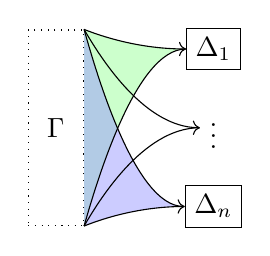
\begin{tikzpicture}[baseline]
    \path
    (-1,1) node (Gtop) {}
    (-1,0) node (G) {$\Gamma$}
    (-1,-1) node (Gbot) {}
    ;
    \node[draw,dotted,fit=(Gtop) (G) (Gbot)] (GG) {};

    \path
    (1,1) node[draw] (Dtop) {$\Delta_1$}
    (1,0) node (D) {$\vdots$}
    (1,-1) node[draw] (Dbot) {$\Delta_n$}
    ;

    \fill[green!20!white,opacity=1] (GG.north east)
    parabola[bend at end] (Dtop.west)
    parabola[bend at start] (GG.south east)
    -- cycle;
    \fill[blue!40!white,opacity=.5] (GG.north east)
    parabola[bend at end] (Dbot.west)
    parabola[bend at start] (GG.south east)
    -- cycle;

    \draw[->] (GG.north east) parabola[bend at end] (Dtop.west);
    \draw (GG.south east) parabola[bend at end] (Dtop.west);
    \draw[->] (GG.north east) parabola[bend at end] (D.west);
    \draw (GG.south east) parabola[bend at end] (D.west);
    \draw[->] (GG.north east) parabola[bend at end] (Dbot.west);
    \draw (GG.south east) parabola[bend at end] (Dbot.west);
  \end{tikzpicture}
\end{displaymath}

To account for usage, we must replace the simple repetition of $\Gamma$ by
repetition of just the types $\gamma$ and \emph{redistribution} of the usage
annotations $\grP$.
Fortunately, our three basic ways of sharing up usage vectors --- zero,
addition, and scaling --- apply directly to the three possible shapes of the
target context --- empty, concatenation, and a usage-annotated singleton.

\begin{definition}[Usage-annotated recursive environment]\label{def:lr-rec-env}
  A \emph{recursive $\V$-environment} between annotated contexts $\Gamma$ and
  $\Delta$ is defined by cases on the shape of $\Delta$ (where
  $\Gamma \env\V_R \Delta$ is the notation for the
  type of recursive environments for given $\V$, $\Gamma$, and $\Delta$):
  \begin{itemize}
    \item There is one environment $\alr{} : \grP\gamma \env\V_R {\cdot}$
      whenever $\grP \leq \gr0$.
    \item For $\rho_l : \grPl\gamma \env\V_R \Delta_l$ and
      $\rho_r : \grPr\gamma \env\V_R \Delta_r$, we have an environment
      $\alr{\rho_l, \rho_r} : \grP\gamma \env\V_R \Delta_l, \Delta_r$ whenever
      $\grP \leq \grPl + \grPr$.
    \item For any value $v : \V\,\grPprime\gamma\,A$, we have an environment
      $\alr{v} : \grP\gamma \env\V_R \gr rA$ whenever
      $\grP \leq \gr r\grPprime$.
  \end{itemize}
\end{definition}

\begin{example}
  Take $\Ann = \plr{\mathbb N, =, 0, +, 1, \times}$, with the equality order
  chosen to avoid any concerns around subsumption of annotations.
  Then, there is an intuitionistic recursive environment as follows, where
  $y\,z$ is the application of $y$ to $z$.
  \[
    \alr{\alr{z},\alr{y\,z}} :
    \plr{x : A, y : B \to C, z : B} \env\vdash_R \plr{B, C}.
  \]
  There is also a usage-aware recursive environment
  \[
    \alr{\alr{z},\alr{y\,z}} :
    \plr{\gr0x : A, \gr2y : B \multimap C, \gr3z : B} \env\vdash_R
    \plr{\gr1B, \gr2C}.
  \]
  The latter relies on the observations that
  $\begin{pmatrix} \gr0 & \gr2 & \gr3 \end{pmatrix} =
  \begin{pmatrix} \gr0 & \gr0 & \gr1 \end{pmatrix}
  + \begin{pmatrix} \gr0 & \gr2 & \gr2 \end{pmatrix}$ and, on the right, that
  $\begin{pmatrix} \gr0 & \gr2 & \gr2 \end{pmatrix} =
  \gr2\begin{pmatrix} \gr0 & \gr1 & \gr1 \end{pmatrix}$.
  Then, we have $\gr0x : A, \gr0y : B \multimap C, \gr1z : B \vdash z : B$ and
  $\gr0x : A, \gr1y : B \multimap C, \gr1z : B \vdash y\,z : C$.
\end{example}

From the example, we can see that the important usage vectors are the initial
one $\begin{pmatrix} \gr0 & \gr2 & \gr3 \end{pmatrix}$ and the usage vectors
at which terms are derived: $\begin{pmatrix} \gr0 & \gr0 & \gr1 \end{pmatrix}$
and $\begin{pmatrix} \gr0 & \gr1 & \gr1 \end{pmatrix}$.
I will call the latter the \emph{leaf vectors}.
The intermediate vector $\begin{pmatrix} \gr0 & \gr2 & \gr2 \end{pmatrix}$ can
be worked out from the leaf vector
$\begin{pmatrix} \gr0 & \gr1 & \gr1 \end{pmatrix}$ and the scaling factor
$\gr2$ found in the codomain context $\gr1B, \gr2C$.
Even when the ordering on annotations is given by a non-equivalence relation
$\leq$, there is a canonical least choice for all of the intermediate vectors,
together with a constraint that the entire linear combination of all the leaf
vectors is less than or equal to the initial usage vector.
In symbols, we may let $\gr\Psi$ be the collection of leaf vectors indexed by
items in $\Delta$, and state
the constraint as $\grP \leq \sum_{\plr{x : \gr rA} \in \Delta} \gr r\gr\Psi_x$.
Seeing $\gr\Psi$ instead as a $\size\Delta \times \size\Gamma$ matrix, this
constraint is $\grP \leq \grQ\gr\Psi$, using vector-matrix multiplication.
The resulting picture is below, showing $\grP$ being split up into $\gr\Psi$,
and then each $\V$-value being constructed in a separate $\gr\Psi_i\gamma$.

\begin{displaymath}
  \begin{tikzpicture}[baseline]
    \path
    (-1,1) node (Gtop) {}
    (-1,0) node (G) {$\grP\gamma$}
    (-1,-1) node (Gbot) {}
    ;
    \node[draw,dotted,fit=(Gtop) (G) (Gbot)] (GG) {};

    \path
    (1,1) node (Dtop) {}
    (1,0) node (D) {$\grQ\delta$}
    (1,-1) node (Dbot) {}
    ;
    \node[draw,dotted,fit=(Dtop) (D) (Dbot)] (DD) {};

    \draw[->,double] (GG) -- (DD);
  \end{tikzpicture}
  \coloneqq
  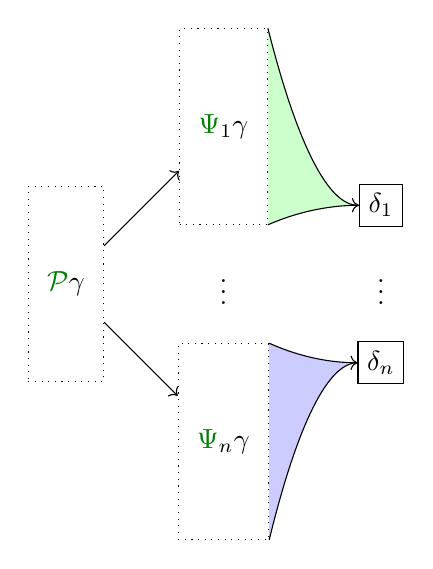
\begin{tikzpicture}[baseline]
    \path
    (-1,1) node (Gtop) {}
    (-1,0) node (G) {$\grP\gamma$}
    (-1,-1) node (Gbot) {}
    ;
    \node[draw,dotted,fit=(Gtop) (G) (Gbot)] (GG) {};

    \path
    (1,3) node (G1top) {}
    (1,2) node (G1) {$\gr\Psi_1\gamma$}
    (1,1) node (G1bot) {}
    ;
    \node[draw,dotted,fit=(G1top) (G1) (G1bot)] (GG1) {};
    \draw[->] (GG) -- (GG1);

    \path (1,0) node {$\vdots$};

    \path
    (1,-1) node (Gntop) {}
    (1,-2) node (Gn) {$\gr\Psi_n\gamma$}
    (1,-3) node (Gnbot) {}
    ;
    \node[draw,dotted,fit=(Gntop) (Gn) (Gnbot)] (GGn) {};
    \draw[->] (GG) -- (GGn);

    \path
    (3,1) node[draw] (Dtop) {$\delta_1$}
    (3,0) node (D) {$\vdots$}
    (3,-1) node[draw] (Dbot) {$\delta_n$}
    ;

    \fill[green!20!white] (GG1.north east)
    parabola[bend at end] (Dtop.west)
    parabola[bend at start] (GG1.south east)
    -- cycle;
    \draw[->] (GG1.north east) parabola[bend at end] (Dtop.west);
    \draw (GG1.south east) parabola[bend at end] (Dtop.west);

    \fill[blue!20!white] (GGn.north east)
    parabola[bend at end] (Dbot.west)
    parabola[bend at start] (GGn.south east)
    -- cycle;
    \draw[->] (GGn.north east) parabola[bend at end] (Dbot.west);
    \draw (GGn.south east) parabola[bend at end] (Dbot.west);
  \end{tikzpicture}
  \quad\textrm{where }\grP \leq \grQ\gr\Psi
\end{displaymath}

From this point, we can recover a functional-style definition of usage-aware
environments.
We choose our leaf vectors $\gr\Psi$ up-front, check the inequality, and then
produce a value at each leaf vector.
%From this definition, we can recover a functional-style definition by
%separating choices of usage vectors from the provision of $\V$-values.
%In particular, the only choices of usage vectors that are essential are the
%$\grPprime$s in the singleton case, with the choices in the concatenation case
%being determined as scalings and sums of these $\grPprime$s.
%I let $\gr\Psi$ collect up these $\size\Delta$-many choices of
%$\size\Gamma$-length usage vectors and note that the constraint on $\gr\Psi$
%generated by all the scaling and summing is
%$\grP = \sum_{\plr{x : \gr rA} \in \Delta} \gr r\gr\Psi_x$.

\begin{definition}[Usage-annotated environment (tentative)]
  A \emph{$\V$-environment} between annotated contexts $\Gamma$ and $\Delta$
  (written $\grP\gamma$ and $\grQ\delta$, respectively, when convenient)
  is a matrix $\gr\Psi : \Ann^{\size\Delta \times \size\Gamma}$ such that
  $\grP \leq \grQ\gr\Psi$ and for each
  $\plr{x : A} \in \delta$ we have a value of type $\V\,\gr\Psi_x\gamma\,A$.
\end{definition}

I find this definition somewhat fiddly because of its reliance on low-level
concepts like non-usage-checked variables and rows of a matrix.
We note that $\gr\Psi_x = \bra x\gr\Psi$, from which point, requiring not
just $\V\,\gr\Psi_x\gamma\,A$ but rather $\V\,\plr{\grQprime\gr\Psi}\gamma\,A$
for any $\grQprime \leq \bra x$ is a minor change (and equivalent if $\V$
respects subusaging, which is practically always the case).
``An $x$ such that $(x : A) \in \delta$ and $\grQprime \leq \bra x\gr\Psi$''
is exactly the definition of $\grQprime\delta \sqni A$.
I further regularise this clause by asking for a
$\grPprime \leq \grQprime\gr\Psi$ rather than $\grQprime\gr\Psi$ exactly,
leaving us needing, for each $\grPprime$ and $\grQprime$ related in the same
way ($\gr\Psi$) as $\grP$ and $\grQ$, a function from $\grQprime\delta \sqni A$
to $\V\,\grPprime\gamma\,A$.
Finally, I choose to switch from matrices and matrix multiplication to
linear maps and their actions, which are easier to work with.
All of these changes yield my primary definition of an environment for
usage-annotated calculi, which will be used for the rest of this chapter and in
\cref{sec:framework}.

\begin{definition}[Usage-annotated environment]\label{def:lr-env}
  A \emph{$\V$-environment} between annotated contexts $\Gamma$ and $\Delta$
  (written $\grP\gamma$ and $\grQ\delta$, respectively, when convenient)
  is a linear map $\gr\Psi : \Ann^{\size\Delta} \to \Ann^{\size\Gamma}$ (written
  postfix) such that $\grP \leq \grQ\gr\Psi$ and for each $A$, $\grPprime$, and
  $\grQprime$ such that $\grPprime \leq \grQprime\gr\Psi$, a function from
  $\grQprime\delta \sqni A$ to $\V\,\grPprime\gamma\,A$.
\end{definition}
\begin{notation}
  When there are multiple environments in question and $\rho$ is such an
  environment, I use the notation $\rho.\gr\Psi$ to refer to $\gr\Psi$.
  For example, $\grP \leq \grQ\plr{\rho.\gr\Psi}$.
  For the action on variables, I write $\rho(x)$, where
  $x : \grQprime\delta \sqni A$.
  The expression ``$\rho(x)$'' alone is ambiguous because of the slack in the
  usage context $\grPprime$ of the resulting value.
  Therefore, I will always make sure $\grPprime$ and $\grQprime$ clear when
  using this notation.
\end{notation}

The following simple lemma shows that usage-annotated environments are, in a
sense, as good as simple environments on usage-checked variables.
What usage-annotated environments give us beyond simple environments is the
ability to accommodate linear decompositions, in a way I will make precise in
the next section.

\begin{lemma}
  We can use an environment $\rho : \Gamma \env\V \Delta$ to map a
  usage-checked variable $x : \Delta \sqni A$ to a value of type
  $\V\,\Gamma\,A$.
\end{lemma}
\begin{proof}
  Let $\Gamma = \grP\gamma$ and $\Delta = \grQ\delta$.
  Set $\grPprime \coloneqq \grP$ and $\grQprime \coloneqq \grQ$, then
  $\grP \leq \grQ\gr\Psi$ by the constraint in $\rho$, so we can take
  the $\V$-value $\rho(x)$.
\end{proof}
\label{sec:lrkits}
  \section{Properties of linear environments}
  I settle on \cref{def:lr-env}, and prove various properties about it.

\begin{lemma}\label{thm:env-resize}
  Given an environment $\rho : \grP\gamma \env\V \grQ\delta$ and a $\grPprime$
  and a $\grQprime$ such that $\grPprime \leq \grQprime\plr{\rho.\gr\Psi}$,
  there is also an environment of type $\grPprime\gamma \env\V \grQprime\delta$
  with the same linear map and action on variables.
\end{lemma}
\begin{proof}
  The only part of the definition of an environment dependent on $\grP$ or
  $\grQ$ is the constraint $\grP \leq \grQ\gr\Psi$, which we are able to
  replace for $\grPprime$ and $\grQprime$.
\end{proof}

When constructing an environment, we can do so by cases on the shape of the
target context.
We can create an environment into the empty context when all usage annotations
on the source context are $\gr0$.
We can create an environment into a concatenated context when we can additively
split up the annotations of the source context and produce environments into
both halves from the split sources.
We can create an environment into a singleton context when there is a context
$\gr r$ times smaller than the source context in which we can produce a value
of the appropriate type.

\begin{lemma}\label{thm:construct-env}
  We can define all of the following equivalences for any values of the free
  variables, assuming that $\V$ respects subusaging (i.e.,
  $\grPprime \leq \grP \to
  \V\,\grP\gamma \rightarrowtriangle \V\,\grPprime\gamma$).
  \begin{itemize}
    \item $I^{\sep} \leftrightarrowtriangle \plr{{-} \env\V {\cdot}}$
    \item $\plr{{-} \env\V \Delta_l} \sep \plr{{-} \env\V \Delta_r}
      \leftrightarrowtriangle \plr{{-} \env\V \Delta_l, \Delta_r}$
    \item $\gr r \cdot \plr{\V\,(-)\,A}
      \leftrightarrowtriangle \plr{{-} \env\V \gr rA}$
  \end{itemize}
\end{lemma}
\begin{proof}
  There are 6 cases to check.
  Throughout, we write $\Gamma$ as $\grP\gamma$ and $\Delta$ as $\grQ\delta$
  when convenient.
  \begin{description}
    \item[$I^{\sep}(\rightarrowtriangle)$]
      Let $\gr\Psi$ be the unique linear map out of the zero space.
      By assumption and definition, $\grP \leq \gr0 = \grQ\gr\Psi$.
      There are no variables to act upon.
    \item[$I^{\sep}(\leftarrowtriangle)$]
      $\grQ\gr\Psi$ is an empty sum, so if $\grP \leq \grQ\gr\Psi$ then
      $\grP \leq \gr0$.
    \item[$\sep(\rightarrowtriangle)$]
      Let the given environments be $\rho_l : \grPl\gamma \env\V \grQl\delta$
      and $\rho_r : \grPr\gamma \env\V \grQr\delta$, with
      $\grP \leq \grPl + \grPr$.
      Define $\gr\Psi \coloneqq [\rho_l.\gr\Psi, \rho_r.\gr\Psi]$, using the
      coproduct structure of the concatenated vector space.
      We have $\grP \leq \grPl + \grPr \leq
      \grQl\plr{\rho_l.\gr\Psi} + \grQr\plr{\rho_r.\gr\Psi} =
      \begin{pmatrix} \grQl & \grQr \end{pmatrix}\gr\Psi$.
      To act on variables, we are given $\grPprime \leq
      \begin{pmatrix} \gr{\grQ'_l} & \gr{\grQ'_r} \end{pmatrix}\gr\Psi$ and
      $\gr{\grQ'_l}\delta_l, \gr{\grQ'_r}\delta_r \sqni A$.
      Without loss of generality, let us have $\gr{\grQ'_l}\delta_l \sqni A$
      and $\gr{\grQ'_r} \leq \gr0$.
      Thus, $\grPprime \leq
      \gr{\grQ'_l}\plr{\rho_l.\gr\Psi} + \gr{\grQ'_r}\plr{\rho_r.\gr\Psi} \leq
      \gr{\grQ'_l}\plr{\rho_l.\gr\Psi}$,
      and we can act on the variable using $\rho_l$.
    \item[$\sep(\leftarrowtriangle)$]
      Let the unnamed context be $\Gamma$, also written $\grP\gamma$.
      The linear map
      $\gr\Psi : \Ann^{\size{\Delta_l} + \size{\Delta_r}} \to \Ann^{\size\Gamma}$
      splits into
      $\gr\Psi_{\gr l} : \Ann^{\size{\Delta_l}} \to \Ann^{\size\Gamma}
      \coloneqq \alr{\id, 0}; \gr\Psi$ and
      $\gr\Psi_{\gr r} : \Ann^{\size{\Delta_r}} \to \Ann^{\size\Gamma}
      \coloneqq \alr{0, \id}; \gr\Psi$, using the product structure of
      the concatenated vector space.
      Let $\grPl \coloneqq \grQl\gr\Psi_{\gr l}$ and
      $\grPr \coloneqq \grQr\gr\Psi_{\gr r}$, by definition satisfying the
      required constraints.
      For the action on variables, let us consider the left environment (with
      the right environment following symmetrically).
      We are given $\gr{\grP'_l} \leq \gr{\grQ'_l}\gr\Psi_{\gr l}$ and
      $\gr{\grQ'_l}\delta_l \sqni A$.
      From these, we get
      $\gr{\grP'_l} \leq \gr{\grQ'_l}\gr\Psi_{\gr l} =
      \begin{pmatrix} \gr{\grQ'_l} & \gr0 \end{pmatrix}\gr\Psi$ and
      $\gr{\grQ'_l}\delta_l, \gr0\delta_r \sqni A$.
      We can therefore act using the original environment.
    \item[$\cdot(\rightarrowtriangle)$]
      Let $\grP$ and $\grPprime$ be such that $\grP \leq \gr r\grPprime$ and let
      $v : \V\,\grPprime\gamma\,A$.
      Let $\gr\Psi : \Ann \to \Ann^{\size\gamma}
      \coloneqq \gr r\gr' \mapsto \gr r\gr'\grPprime$.
      By definition and the previous assumption, we have
      $\grP \leq \gr r\gr\Psi$.
      When acting on a variable, we have $\grP\gr{''} \leq \gr r\gr'\gr\Psi$
      and $\gr r\gr'A \sqni A'$.
      The latter tells us that $A = A'$ and $\gr r\gr' \leq \gr1$.
      Thus, $\grP\gr{''} \leq \grPprime$.
      Therefore, by subusaging, we may produce a value of type
      $\V\,\grPprime\gamma\,A$, which we can take to be $v$.
    \item[$\cdot(\leftarrowtriangle)$]
      Let us have an environment of type $\grP\gamma \env\V \gr rA$.
      We want to use its action on variables to yield a value.
      To do this, we let $\grPprime \coloneqq \gr1\gr\Psi$, and use this
      equation, together with the fact that we have a variable of type
      $\gr1A \sqni A$, to get a value of type $\V\,\grPprime\gamma\,A$.
      Furthermore, we derive $\grP \leq \gr r\gr\Psi = \gr r\grPprime$, as
      required.
  \end{description}
\end{proof}

We could, as in \cref{def:lr-rec-env}, use these three clauses to define what an
environment is.
However, such a definition appears to require creative induction hypotheses in
the proving of simple lemmas, in contrast to the more direct proofs I achieve
below using \cref{def:lr-env}.
To take a concrete example, consider how we may construct an ``identity''
environment of type $\Gamma \env\V \Gamma$, as in \cref{thm:env-id} below.
If we try to directly proceed by induction on $\Gamma$, we get to the case where
we are aiming to construct an environment of type
$\grP\gamma, \grQ\delta \env\V \grP\gamma, \grQ\delta$ by constructing
environments of types $\grP\gamma, \gr0\delta \env\V \grP\gamma$ and
$\gr0\gamma, \grQ\delta \env\V \grQ\delta$.
These are not identity environments, and thus do not come from the hypotheses of
a simple induction.
In contrast, using \cref{def:lr-env}, in \cref{thm:env-id} we are able to use
the standard fact that there are identity linear maps, and on top of such a map
worry only about the value assigned to each variable.

One of the primary test cases for environments is simultaneous substitution,
which will look like the \TirName{sub} rule below.
Note that we have taken $\V \coloneqq {\vdash}$ --- i.e.\ that the values
yielded by the environment are terms, namely the terms to be substituted in for
the free variables of the derivation of $\Delta \vdash A$.

\begin{displaymath}
  \begin{prooftree}
    \hypo{\Gamma \env{\vdash} \Delta}
    \hypo{\Delta \vdash A}
    \infer2[sub]{\Gamma \vdash A}
  \end{prooftree}
\end{displaymath}

The admissibility of substitution will be by induction on the derivation of
$\Delta \vdash A$, so we will need to be able to adapt any environment we are
given to work with any possible context of new premises yielded by the rules of
\cref{fig:lr-bunched}.
In the simply typed case, the only change to the context we encountered was the
binding of new variables.
With usage annotations, we furthermore have linear decompositions of the
context, necessitating changes to the environment whenever usage annotations
change.

There are three kinds of linear decompositions we have to deal with: zero,
addition, and scaling; corresponding to bunched connectives $I^*$, $\sep$, and
$\gr r \cdot {}$, respectively.
In each of these three cases, we have a simple preservation lemma, transforming
an environment
of type $\Gamma \env\V \Delta$ and a decomposition of $\Delta$ into a
decomposition of $\Gamma$ and environments for all of the decomposed fragments
of $\Gamma$ and $\Delta$.

\begin{lemma}[environments preserve zero]\label{thm:lr-env-zero}
  Given an environment $\rho : \grP\gamma \env\V \grQ\delta$ such that
  $\grQ \leq \gr 0$, we also have that $\grP \leq \gr 0$.
\end{lemma}
\begin{proof}
  $\grP \leq \grQ\gr\Psi \leq \gr0\gr\Psi = \gr0$, by environment
  compatibility from $\rho$ and monotonicity and linearity of $\gr\Psi$.
\end{proof}

\begin{lemma}[environments preserve addition]\label{thm:lr-env-add}
  Given an environment $\rho : \grP\gamma \env\V \grQ\delta$ such that
  $\grQ \leq \grQl + \grQr$ for some $\grQl$ and $\grQr$, we also have $\grPl$
  and $\grPr$ such that $\grP \leq \grPl + \grPr$ and there are environments
  $\rho_l : \grPl\gamma \env\V \grQl\delta$ and
  $\rho_r : \grPr\gamma \env\V \grQr\delta$.
\end{lemma}
\begin{proof}
  Let $\grPl \coloneqq \grQl\gr\Psi$ and $\grPr \coloneqq \grQr\gr\Psi$.
  Then, $\grP \leq \grQ\gr\Psi \leq \plr{\grQl + \grQr}\gr\Psi =
  \grQl\gr\Psi + \grQr\gr\Psi = \grPl + \grPr$, satisfying the first condition.
  Because clearly $\grPl \leq \grQl\gr\Psi$ and $\grPr \leq \grQr\gr\Psi$,
  applying \cref{thm:env-resize} to $\rho$ gives us the required
  new environments $\rho_l$ and $\rho_r$.
\end{proof}

\begin{lemma}[environments preserve scaling]\label{thm:lr-env-scale}
  Given an environment $\rho : \grP\gamma \env\V \grQ\delta$ such that
  $\grQ \leq \gr r\grQprime$ for some $\grQprime$, we also have a $\grPprime$
  such that $\grP \leq \gr r\grPprime$ and there is an environment
  $\rho' : \grPprime\gamma \env\V \grQprime\delta$.
\end{lemma}
\begin{proof}
  Let $\grPprime \coloneqq \grQprime\gr\Psi$.
  Then, $\grP \leq \grQ\gr\Psi \leq \plr{\gr r\grQprime}\gr\Psi =
  \gr r\plr{\grQprime\gr\Psi} = \gr r\grPprime$, satisfying the first condition.
  Because clearly $\grPprime \leq \grQprime\gr\Psi$,
  applying \cref{thm:env-resize} to $\rho$ gives us the required
  new environment $\rho'$.
\end{proof}

The final change environments need to preserve is the binding of new free
variables.
In \cref{sec:syntactic-kits}, we had the operation \AgdaFunction{bindEnv} for
this purpose in the intuitionistic setting.
There, we relied on $\V$ supporting a map from $\ni$-variables and admitting
weakening.
In the usage-annotated setting, the former requirement is updated to having a
map from usage-checked $\sqni$-variables.
As for the latter requirement, it turns out that we only need $\V$ to admit
weakening by $\gr0$-annotated variables, which is much more reasonable than
general weakening.
\Cref{thm:lr-bind} adapts \AgdaFunction{bindEnv} for the usage-annotated
setting.

\begin{lemma}[\AgdaFunction{bindEnv}]\label{thm:lr-bind}
  Given functions
  ${\swarrow^k} : \forall \Gamma, \grR, \theta.~\grR \leq \gr0 \to
  \V\,\Gamma \rightarrowtriangle \V\,\plr{\Gamma, \grR\theta}$ and
  $\mathrm{vr} : {\sqni} \rightarrowtriangle \V$, we can turn an environment of
  type $\Gamma \env\V \Delta$ into an environment of type
  $\Gamma, \Theta \env\V \Delta, \Theta$ for any context $\Theta$.
\end{lemma}
\begin{proof}
  Let $\grP\gamma \coloneqq \Gamma$, $\grQ\delta \coloneqq \Delta$, and
  $\grR\theta \coloneqq \Theta$.
  Let the new linear map $\gr\Psi\gr' : \Ann^{\size\Delta + \size\Theta} \to
  \Ann^{\size\Gamma + \size\Theta}$ be $\gr\Psi \oplus \gr I$.
  That is, in block matrix notation,
  $\begin{pmatrix} \gr\Psi & \gr0 \\ \gr0 & \gr I \end{pmatrix}$.
  Checking that this linear map fits, we have
  $\begin{pmatrix}\grP & \grR\end{pmatrix}
  \leq \begin{pmatrix}\grQ\gr\Psi & \grR\gr I\end{pmatrix}
  = \begin{pmatrix}\grQ & \grR\end{pmatrix}\plr{\gr\Psi \oplus \gr I}$.
  For the action on variables, we are given vectors $\grPprime$,
  $\grR\gr'_\grP$, $\grQprime$, and $\grR\gr'_\grQ$ such that
  $\begin{pmatrix} \grPprime & \grR\gr'_\grP \end{pmatrix} \leq
  \begin{pmatrix} \grQprime & \grR\gr'_\grQ \end{pmatrix}
  \plr{\gr\Psi \oplus \gr I}$ and we have a variable of type
  $\grQprime\delta, \grR\gr'_\grQ\theta \sqni A$ for some type $A$.
  The constraint on the new vectors reduces to $\grPprime \leq \grQprime\gr\Psi$
  and $\grR\gr'_\grP \leq \grR\gr'_\grQ$.
  From the variable we either have a variable $x$ in $\delta$ with
  $\grQprime \leq \langle x \rvert$ and $\grR\gr'_\grQ \leq \gr0$, or a
  variable $y$ in $\theta$ with $\grQprime \leq \gr0$ and
  $\grR\gr'_\grQ \leq \langle y \rvert$.
  In the former case, the action of the original environment on $x$ gives us a
  $\V$-value in $\grPprime\gamma$, and the $\gr0$-weakening principle
  $\swarrow^k$, noting that $\grR\gr'_\grP \leq \grR\gr'_\grQ \leq \gr0$, gives
  us a $\V$-value in $\grPprime\gamma, \grR\gr'_\grP\theta$.
  In the latter case, we have that
  $\begin{pmatrix} \grPprime & \grR\gr'_\grP \end{pmatrix}
  \leq \begin{pmatrix} \grQprime\gr\Psi & \grR\gr'_\grQ \end{pmatrix}
  \leq \begin{pmatrix} \gr0\gr\Psi & \langle y \rvert \end{pmatrix}
  = \begin{pmatrix} \gr0 & \langle y \rvert \end{pmatrix}
  = \left\langle {\searrow}y \right\rvert$, so $y$ also serves as a
  usage-checked variable in $\grPprime\gamma, \grR\gr'_\grP\theta$.
  From this usage-checked variable, we get a $\V$-value in the same context
  using $\mathrm{vr}$.
\end{proof}

I put together the preceding pieces to give a syntactic traversal operation over
$\name$ in the following section.
For the rest of this section, I observe some more constructions purely on
environments --- in particular, composition of environments given certain
assumptions about the families of values.

Following \citet{ACU15}, we expect (intuitionistic) ST$\lambda$C syntax to form
a relative monad over $\ni$ seen as a functor from the category of contexts
under renaming to the functor category $\blr{\mathrm{Ty}, \Set}$, where
$\mathrm{Ty}$ is the discrete category of ST$\lambda$C types.
Notice that, given $F,G : \blr{\mathrm{Ty}, \Set}$, a morphism from $F$ to $G$
is a function of type $F \rightarrowtriangle G$ (with naturality being trivial).
Therefore, we expect a relative monad, given as a Kleisli triple, to have a unit
$\eta_\Gamma : \Gamma \ni \plr{-} \rightarrowtriangle \Gamma \vdash \plr{-}$
given by the variable rule, and a Kleisli extension operator
${^*}_{\Gamma,\Delta} :
\plr{\Gamma \ni \plr{-} \rightarrowtriangle \Delta \vdash \plr{-}} \to
\plr{\Gamma \vdash \plr{-} \rightarrowtriangle \Delta \vdash \plr{-}}$
given by substitution.
Composition of substitutions falls out of this framework as Kleisli composition.
However, in the usage-aware case, substitution needs not just a mapping of
variables $f : \Gamma \sqni \plr{-} \rightarrowtriangle \Delta \vdash \plr{-}$,
but rather an environment $\rho : \Delta \env\vdash \Gamma$, as we have already
discussed.
It therefore makes sense for our replacement for the Kleisli extension operator
to similarly take an environment rather than a simple variable mapping.

\Cref{thm:env-comp} below amounts to deriving a modified notion of Kleisli
composition from a modified Kleisli extension.
Additionally, \cref{thm:env-id} is required to turn a monadic unit into an
identity environment.
Both lemmas are stated in terms of general $\U$/$\V$/$\W$-environments, with
some specific examples (e.g.\ for renaming and substitution) below them.

\begin{lemma}[Identity environment]\label{thm:env-id}
  Given a function
  \[
    \mathrm{vr}_{\Gamma'} :
    \Gamma' \sqni \plr{-} \rightarrowtriangle \V\,\Gamma'
  \]
  for any
  $\Gamma$ we have an environment $\mathrm{id} : \Gamma \env\V \Gamma$.
\end{lemma}
\begin{proof}
  Let $\Gamma = \grP\gamma$.
  Let $\gr\Psi$ be the identity map, which clearly satisfies
  $\grP \leq \grP\gr\Psi$.
  When acting on a variable, the inequality $\grPprime \leq \grQprime\gr\Psi$
  means that $\grPprime \leq \grQprime$.
  We are given a variable of type $\grQprime\gamma \sqni A$, which we can
  coerce to a variable of type $\grPprime\gamma \sqni A$, upon which we apply
  $\mathrm{vr}$ to get the required value of type $\V\,\grPprime\gamma\,A$.
\end{proof}

\begin{lemma}[Composition of environments]\label{thm:env-comp}
  Given a function
  \[
    \mathrm{lift}_{\Gamma', \Delta'} :
    \Gamma' \env\U \Delta' \to \V\,\Delta' \rightarrowtriangle \W\,\Gamma'
  \]
  we can compose environments $\rho : \Gamma \env\U \Delta$ and
  $\sigma : \Delta \env\V \Theta$ into an environment
  $\rho \gg \sigma : \Gamma \env\W \Theta$.
\end{lemma}
\begin{proof}
  Let $\Gamma = \grP\gamma$, $\Delta = \grQ\delta$, and $\Theta = \grR\theta$.
  Take $\gr\Psi$ to be the composition $\plr{\sigma.\gr\Psi}\plr{\rho.\gr\Psi}$,
  noting that
  $\grP \leq \grQ\plr{\rho.\gr\Psi} \leq
  (\grR\plr{\sigma.\gr\Psi})\plr{\rho.\gr\Psi} = \grR\gr\Psi$
  thanks to the inequalities yielded by $\sigma$ and $\rho$.
  When acting on a variable, we are given $\grPprime \leq \grRprime\gr\Psi$ and
  a variable $v : \grRprime\theta \sqni A$, and want a value of type
  $\W\,\grPprime\gamma\,A$.
  Let $\grQprime \coloneqq \grRprime\plr{\sigma.\gr\Psi}$, with inequality
  $\grQprime \leq \grRprime\plr{\sigma.\gr\Psi}$ giving us a value
  $\sigma(v) : \V\,\grQprime\delta\,A$.
  We wish to apply $\mathrm{lift}$ to $\sigma(v)$ with
  $\Gamma' \coloneqq \grPprime\gamma$ and $\Delta' \coloneqq \grQprime\delta$ to
  complete the construction of the $\W$-value.
  To do this, we need an environment of type
  $\grPprime\gamma \env\U \grQprime\delta$, which we can get from $\rho$ using
  \cref{thm:env-resize}, noting that
  $\grPprime \leq \grRprime\plr{\sigma.\gr\Psi}\plr{\rho.\gr\Psi} =
  \grQprime\plr{\rho.\gr\Psi}$.
\end{proof}

We can derive the following corollaries as instances of environment composition.

\begin{corollary}[Composition of renamings]\label{thm:ren-comp}
  Given renamings $\rho : \Gamma \env\sqni \Delta$ and
  $\sigma : \Delta \env\sqni \Theta$, we can form their composite
  $\rho; \sigma : \Gamma \env\sqni \Theta$.
\end{corollary}
\begin{proof}
  Take $\U = \V = \W = {\sqni}$ in \cref{thm:env-comp}.
  Then let $\mathrm{lift}\,\rho\,x \coloneqq \rho(x)$.
\end{proof}

\begin{corollary}[Post-composition with a renaming]\label{thm:ren-env-comp}
  Given an environment $\rho : \Gamma \env\U \Delta$ and a renaming
  $\sigma : \Delta \env\sqni \Theta$, we can form their composite
  $\rho; \sigma : \Gamma \env\U \Theta$.
\end{corollary}
\begin{proof}
  As in \cref{thm:ren-comp}.
\end{proof}

\begin{corollary}[Pointwise renaming of an environment]\label{thm:env-ren}
  If $\sdtstile{}\V$ respects renaming, then so does $\env\V$ (on the left).
\end{corollary}
\begin{proof}
  Suppose we have $\rho : \Gamma \env\sqni \Delta$ and
  $\sigma : \Delta \env\V \Theta$.
  We want to compose these via \cref{thm:env-comp} with $U = {\sqni}$ and
  $\V = \W$.
  The function $\mathrm{lift}$ is given exactly by the fact that $\V$ respects
  renaming.
\end{proof}

\begin{corollary}[Composition of substitutions]\label{thm:sub-comp}
  Given substitutions $\rho : \Gamma \env\vdash \Delta$ and
  $\sigma : \Delta \env\vdash \Theta$, we can form their composite
  $\rho; \sigma : \Gamma \env\vdash \Theta$.
\end{corollary}
\begin{proof}
  Take $\U = \V = \W = {\vdash}$ in \cref{thm:env-comp}.
  Then, $\mathrm{lift}$ is given by the action of a substitution on a term
  (see \AgdaFunction{sub} in the following section).
\end{proof}

\begin{corollary}[Composing semantics with substitution]
  If we have a semantics (in the sense of \cref{sec:gen-sem} and
  \cref{sec:traversal}) from $\U$ to $\W$, then from an environment
  $\rho : \Gamma \env\U \Delta$ and a substitution
  $\sigma : \Delta \env\vdash \Theta$, we can form the composite
  $\rho; \sigma : \Gamma \env\W \Theta$.
\end{corollary}

% Concatenation is difficult; save to after I've talked about renamings.

% Finally for this section, we give the conditions under which the
% context-forming operations (empty, concatenation, and singleton) have a
% functorial action with respect to $\V$-environments.
%
% \begin{lemma}
%   For any $\V$, there is an environment ${\cdot} \env\V {\cdot}$.
% \end{lemma}
% \begin{proof}
%   By \cref{thm:construct-env}, it suffices to show $I\,{\cdot}$, which is
%   trivially true.
% \end{proof}
\label{sec:lenv}
  \section{Substitution is admissible in \name{}}
  \def\LRKits{../agda/processed-latex/LRKits.tex}

I now show that, using the notion of \emph{environment} derived in
\cref{sec:lrkits}, we can replicate the Agda proofs from
\cref{sec:syntactic-kits} in the usage-aware setting of $\name$.
From \cref{sec:lenv}, we know that environments are preserved under all
syntax-forming operations: zero, addition, scaling, and binding.
What is left is to show how these properties are deployed, and also how to
go on and prove the admissibility of simultaneous renaming, simultaneous
substitution, and then single substitution.

There are a few notational changes necessary in the Agda code, compared to the
typeset mathematics above.
Usage vectors, elsewhere called $\grP$, $\grQ$, and $\grR$ are rendered as
\AgdaBound{P}, \AgdaBound{Q}, and \AgdaBound{R}, respectively.
Usage contexts and typing contexts are tied together with the
\AgdaInductiveConstructor{ctx} constructor, rather than simple juxtaposition.
Environments, elsewhere notated $\Gamma \env\V \Delta$, are rendered as
\AgdaRecord{[}\AgdaSpace{}\AgdaBound{$\V$}\AgdaSpace{}\AgdaRecord{]}%
\AgdaSpace{}\AgdaBound{$\Gamma$}\AgdaSpace{}\AgdaRecord{$\Rightarrow^e$}%
\AgdaSpace{}\AgdaBound{$\Delta$}.

I start with the definition \AgdaFunction{Weakening}, which says what it means
for a family of values \AgdaBound{$\V$} to respect one step of weakening on the
right by $\gr0$-use variables.
I state weakening in a slightly different way to what appears in the statement
of \cref{thm:lr-bind}, so as to help
unification against a known result type (avoiding the problem described by
\citet{McBride12} as \emph{green slime}).
The type \AgdaFunction{Weakening}\AgdaSpace{}\AgdaBound{$\V$} can be read as
saying that, for any context $\grP\gamma$ of shape $s + t$, if the right of
$\grP$ is below $\gr0$, then a value in the left part of $\grP\gamma$ weakens
to a value in the whole of $\grP\gamma$.

\ExecuteMetaData[\LRKits]{Weakening}

Given this new definition of \AgdaFunction{Weakening}, the record
\AgdaRecord{Kit} remains largely unchanged relative to what we saw in
\cref{sec:syntactic-kits}.
We still want $\V$-values to respect weakening (as used in \cref{thm:lr-bind}),
and to support maps \AgdaField{vr} from variables (also used in
\cref{thm:lr-bind}) and \AgdaField{tm} into terms (used when traversal reaches a
variable, we get a value from the environment, and want to produce a term from
that value).
As well as \AgdaFunction{Weakening}, note that \AgdaRecord{\_$\sqni$\_} and, of
course, \AgdaDatatype{\_$\vdash$\_} have different definitions to the
corresponding intuitionistic notions, but they still represent morally the same
parts of the language and its metatheory.

\ExecuteMetaData[\LRKits]{Kit}

To demonstrate the important points succinctly, I cut \name{} down to just the
$\oc\gr r$-fragment.
The introduction rule and pattern-matching eliminator feature scaling, addition,
and variable binding, missing out only on sharing (which is trivial) and zero
(which is simpler than, and analogous to, addition).
The resulting type of well typed terms is below.

\ExecuteMetaData[\LRKits]{Tm}

Given a \AgdaRecord{Kit}\AgdaSpace{}\AgdaBound{$\V$},
\cref{thm:lr-bind} gives a function with the following type.

\ExecuteMetaData[\LRKits]{bindEnv}

Given \AgdaFunction{bindEnv} (\cref{thm:lr-bind}), \AgdaFunction{env-+}
(\cref{thm:lr-env-add}), and \AgdaFunction{env-*} (\cref{thm:lr-env-scale}),
we can reproduce the syntactic traversal \AgdaFunction{trav}.
Similarly to the unchanged high-level definition of \AgdaRecord{Kit}, we are
aiming for an unchanged traversal principle expressed by the rule below.
When $\V$ has a \AgdaRecord{Kit} structure, and we have a $\V$-environment from
$\Gamma$ to $\Delta$, we can transform a term in $\Delta$ to a term in $\Gamma$
of the same type.

\[
  \begin{prooftree}
    \hypo{\text{\AgdaRecord{Kit}\AgdaSpace{}}\V}
    \hypo{\Gamma \env\V \Delta}
    \hypo{\Delta \vdash A}
    \infer3[Trav]{\Gamma \vdash A}
  \end{prooftree}
\]

With all the lemmas of \cref{sec:lenv} in place, writing \AgdaFunction{trav}
becomes routine.
When processing a rule, we work our way up through the
premise connectives, applying \AgdaFunction{env-*} wherever we see a
\AgdaFunction{$\cdot^c$}, \AgdaFunction{env-+} wherever we see a
\AgdaFunction{$*^c$}, and \AgdaFunction{bindEnv} wherever we see a
\AgdaFunction{Bind}.
We then use whatever environments (with names beginning with
\AgdaBound{$\rho$}) and whatever usage vector splitting facts (with names
beginning with \AgdaBound{sp}) come out of this process to recursively
traverse the subterms and recombine the results.

\ExecuteMetaData[\LRKits]{trav}

Instantiating the generic syntactic traversal \AgdaFunction{trav} to renaming
looks just like it did in the intuitionistic case.
I have consistently replaced intuitionistic variables by linear variables, so
\AgdaFunction{id} and \AgdaInductiveConstructor{var} still work to embed
variables into variables and terms, respectively.
Weakening for variables \AgdaFunction{$\swarrow^v$} (not pictured) has been
updated to note that, for $\grP \leq \bra x$ and $\grR \leq \gr0$, we also have
$\begin{pmatrix} \grP & \grR \end{pmatrix} \leq \bra{{\swarrow}x}$.

\ExecuteMetaData[\LRKits]{var-kit}

In the intuitionistic case, environments were just functions, so we passed the
variable weakening function \AgdaFunction{$\swarrow^v$} to the function
\AgdaFunction{ren} to yield a term weakening function.
However, a usage-aware environment is a function packed together with usage
distribution data.
As such, we must make an environment version of \AgdaFunction{$\swarrow^v$}.
I start with a general lemma \AgdaFunction{$\swarrow$\^{}Env}, stating that if
$\V$ supports weakening, then so do $\V$-environments (in their domain
context).
This lemma then specialises to variables, with the identity renaming
\AgdaFunction{id\^{}Env} on the left part of the context and the proof
\AgdaBound{R0} that the right part of the context is below $\gr0$ combining
to give the desired weakening environment.

\ExecuteMetaData[\LRKits]{dlv-env}

This is what we need to instantiate \AgdaFunction{trav} for substitution.
As a reminder, I also give the type of \AgdaFunction{sub} in rule form.

\ExecuteMetaData[\LRKits]{sub}
\[
  \ebrule{%
    \hypo{\Gamma \env\vdash \Delta}
    \hypo{\Delta \vdash B}
    \infer2[sub]{\Gamma \vdash B}
  }
\]

Finally, the simultaneous substitution \AgdaFunction{sub} specialises to
single substitution.

\begin{corollary}[Single substitution]\label{thm:single-sub}
  The following equivalent rules are admissible.
  \begin{mathpar}
    \ebrule{%
      \hypo{\grR \leq \gr r\grP + \grQ}
      \hypo{\grP\gamma \vdash A}
      \hypo{\grQ\gamma, \gr rA \vdash B}
      \infer3{\grR\gamma \vdash B}
    }
    \and
    \ebrule[comb]{%
      \hypo{\gr r \cdot \plr{{} \vdash A}}
      \hypo{\sep}
      \hypo{\gr rA \vdash B}
      \infer3{{} \vdash B}
    }
  \end{mathpar}
\end{corollary}
\begin{proof}
  It is enough to construct a substitution of type
  $\grR\gamma \env\vdash \grQ\gamma, \gr rA$.
  To do this, we use \cref{thm:construct-env} cases $\sep(\rightarrowtriangle)$
  and $\cdot(\rightarrowtriangle)$ on inequalities
  $\grR \leq \grQ + \gr r\grP$ and $\gr r\grP \leq \gr r\grP$ respectively to
  leave us needing a substitution of type $\grQ\gamma \env\vdash \grQ\gamma$ and
  a term of type $\grP\gamma \vdash A$.
  For the substitution, we give the identity substitution (\cref{thm:env-id}),
  and we have the term as a hypothesis.
\end{proof}


\chapter{Weighted multicategories}
  \section{Ordinary and Cartesian multicategories}
  In type theory and categorical logic, the idea of multicategories is to give
an algebraic structure that is close to the syntax of type theory.
In simple type theory, sequents take the form $\Gamma \vdash A$, where $A$ is
the type of the conclusion and $\Gamma$ is a list of types, one type for each
assumption.
Intuitively, a term with assumptions $\Gamma$ and type $A$ constitutes a
morphism from $\Gamma$ to $A$.
Multicategories make this structure --- domains being lists of objects and
codomains being a single object --- part of the definition of morphisms.

\begin{definition}[multicategory]
  A \emph{multicategory} comprises a collection of objects $\obj$, for each
  list of objects $\Gamma$ and object $A$ a set of (multi)morphisms
  $\hom(\Gamma, A)$, and the following morphisms, satisfying the following
  axioms.

  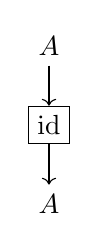
\begin{tikzpicture}
    \path
    (0,1) node(s) {$A$}
    (0,0) node[draw](id) {$\id$}
    (0,-1) node(t) {$A$}
    ;

    \draw[->] (s) -- (id);
    \draw[->] (id) -- (t);
  \end{tikzpicture}
  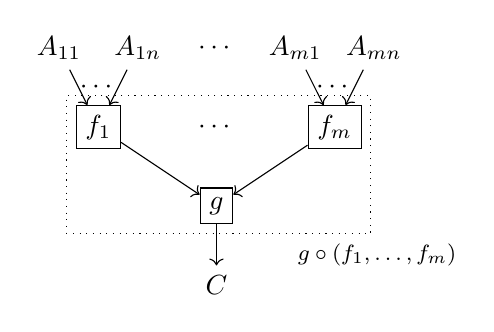
\begin{tikzpicture}
    \path
    (-2,2) node(A11) {$A_{11}$}
    (-1.5,1.5) node(A1dots) {$\cdots$}
    (-1,2) node(A1n) {$A_{1n}$}
    (0,2) node(Adots) {$\cdots$}
    (1,2) node(Am1) {$A_{m1}$}
    (1.5,1.5) node(Amdots) {$\cdots$}
    (2,2) node(Amn) {$A_{mn}$}

    (-1.5,1) node[draw](f1) {$f_1$}
    (0,1) node(fdots) {$\cdots$}
    (1.5,1) node[draw](fm) {$f_m$}

    (0,0) node[draw](g) {$g$}

    (0,-1) node(C) {$C$}
    ;

    \node[draw,dotted,fit=(f1) (fm) (g),
    label=below right:{\footnotesize$g \circ (f_1, \ldots, f_m)$}] (box) {};

    \draw[->] (A11) -- (f1);
    \draw[->] (A1n) -- (f1);
    \draw[->] (Am1) -- (fm);
    \draw[->] (Amn) -- (fm);
    \draw[->] (f1) -- (g);
    \draw[->] (fm) -- (g);
    \draw[->] (g) -- (C);
  \end{tikzpicture}

  \begin{displaymath}
    \begin{matrix}
      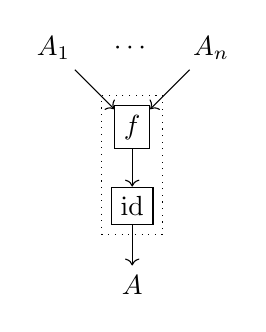
\begin{tikzpicture}[baseline]
        \path
        (-1,2) node(A1) {$A_1$}
        (0,2) node(Adots) {$\cdots$}
        (1,2) node(An) {$A_n$}
        (0,1) node[draw](f) {$f$}
        (0,0) node[draw](id) {$\id$}
        (0,-1) node(t) {$A$}
        ;

        \node[draw,dotted,fit=(f) (id)] {};

        \draw[->] (A1) -- (f);
        \draw[->] (An) -- (f);
        \draw[->] (f) -- (id);
        \draw[->] (id) -- (t);
      \end{tikzpicture}
      =
      \begin{tikzpicture}[baseline]
        \path
        (-1,1) node(A1) {$A_1$}
        (0,1) node(Adots) {$\cdots$}
        (1,1) node(An) {$A_n$}
        (0,0) node[draw](f) {$f$}
        (0,-1) node(t) {$A$}
        ;

        \draw[->] (A1) -- (f);
        \draw[->] (An) -- (f);
        \draw[->] (f) -- (t);
      \end{tikzpicture}
      &\phantom{mmmm}&
      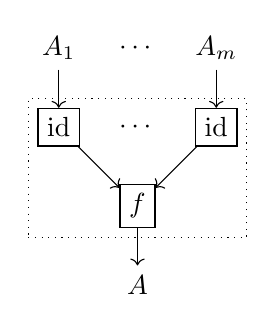
\begin{tikzpicture}[baseline]
        \path
        (-1,2) node(A1) {$A_1$}
        (0,2) node(Adots) {$\cdots$}
        (1,2) node(Am) {$A_m$}
        (-1,1) node[draw](id1) {$\id$}
        (0,1) node(iddots) {$\cdots$}
        (1,1) node[draw](idm) {$\id$}
        (0,0) node[draw](f) {$f$}
        (0,-1) node(t) {$A$}
        ;

        \node[draw,dotted,fit=(id1) (idm) (f)] {};

        \draw[->] (A1) -- (id1);
        \draw[->] (Am) -- (idm);
        \draw[->] (id1) -- (f);
        \draw[->] (idm) -- (f);
        \draw[->] (f) -- (t);
      \end{tikzpicture}
      =
      \begin{tikzpicture}[baseline]
        \path
        (-1,1) node(A1) {$A_1$}
        (0,1) node(Adots) {$\cdots$}
        (1,1) node(An) {$A_n$}
        (0,0) node[draw](f) {$f$}
        (0,-1) node(t) {$A$}
        ;

        \draw[->] (A1) -- (f);
        \draw[->] (An) -- (f);
        \draw[->] (f) -- (t);
      \end{tikzpicture}
    \end{matrix}
  \end{displaymath}

  \begin{displaymath}
    \begin{matrix}
      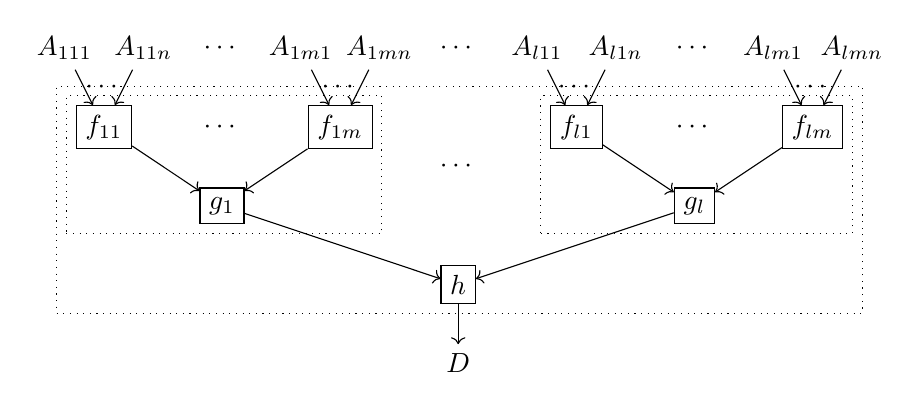
\begin{tikzpicture}
        \path
        % left
        (-5,2) node(A111) {$A_{111}$}
        (-4.5,1.5) node(A1dots) {$\cdots$}
        (-4,2) node(A11n) {$A_{11n}$}
        (-3,2) node(Adots) {$\cdots$}
        (-2,2) node(A1m1) {$A_{1m1}$}
        (-1.5,1.5) node(Amdots) {$\cdots$}
        (-1,2) node(A1mn) {$A_{1mn}$}

        (-4.5,1) node[draw](f11) {$f_{11}$}
        (-3,1) node(fdots) {$\cdots$}
        (-1.5,1) node[draw](f1m) {$f_{1m}$}

        (-3,0) node[draw](g1) {$g_1$}

        % right
        (1,2) node(Al11) {$A_{l11}$}
        (1.5,1.5) node(A1dots) {$\cdots$}
        (2,2) node(Al1n) {$A_{l1n}$}
        (3,2) node(Adots) {$\cdots$}
        (4,2) node(Alm1) {$A_{lm1}$}
        (4.5,1.5) node(Amdots) {$\cdots$}
        (5,2) node(Almn) {$A_{lmn}$}

        (1.5,1) node[draw](fl1) {$f_{l1}$}
        (3,1) node(fdots) {$\cdots$}
        (4.5,1) node[draw](flm) {$f_{lm}$}

        (3,0) node[draw](gl) {$g_l$}

        % middle
        (0,2) node {$\cdots$}
        (0,0.5) node {$\cdots$}
        (0,-1) node[draw](h) {$h$}
        (0,-2) node(D) {$D$}
        ;

        \node[draw,dotted,fit=(f11) (f1m) (g1)] (box1) {};
        \node[draw,dotted,fit=(fl1) (flm) (gl)] (boxl) {};
        \node[draw,dotted,fit=(box1) (boxl) (h)] (box) {};

        \draw[->] (A111) -- (f11);
        \draw[->] (A11n) -- (f11);
        \draw[->] (A1m1) -- (f1m);
        \draw[->] (A1mn) -- (f1m);
        \draw[->] (f11) -- (g1);
        \draw[->] (f1m) -- (g1);
        \draw[->] (g1) -- (h);

        \draw[->] (Al11) -- (fl1);
        \draw[->] (Al1n) -- (fl1);
        \draw[->] (Alm1) -- (flm);
        \draw[->] (Almn) -- (flm);
        \draw[->] (fl1) -- (gl);
        \draw[->] (flm) -- (gl);
        \draw[->] (gl) -- (h);

        \draw[->] (h) -- (D);
      \end{tikzpicture}
      \\=\\
      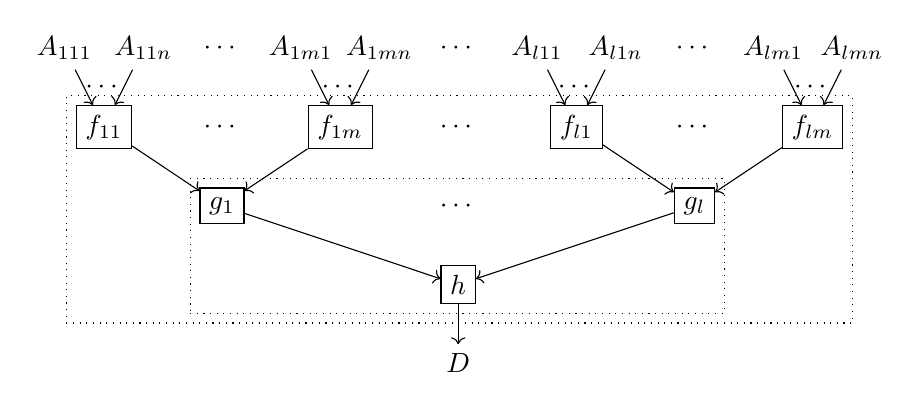
\begin{tikzpicture}
        \path
        % left
        (-5,2) node(A111) {$A_{111}$}
        (-4.5,1.5) node(A1dots) {$\cdots$}
        (-4,2) node(A11n) {$A_{11n}$}
        (-3,2) node(Adots) {$\cdots$}
        (-2,2) node(A1m1) {$A_{1m1}$}
        (-1.5,1.5) node(Amdots) {$\cdots$}
        (-1,2) node(A1mn) {$A_{1mn}$}

        (-4.5,1) node[draw](f11) {$f_{11}$}
        (-3,1) node(fdots) {$\cdots$}
        (-1.5,1) node[draw](f1m) {$f_{1m}$}

        (-3,0) node[draw](g1) {$g_1$}

        % right
        (1,2) node(Al11) {$A_{l11}$}
        (1.5,1.5) node(A1dots) {$\cdots$}
        (2,2) node(Al1n) {$A_{l1n}$}
        (3,2) node(Adots) {$\cdots$}
        (4,2) node(Alm1) {$A_{lm1}$}
        (4.5,1.5) node(Amdots) {$\cdots$}
        (5,2) node(Almn) {$A_{lmn}$}

        (1.5,1) node[draw](fl1) {$f_{l1}$}
        (3,1) node(fdots) {$\cdots$}
        (4.5,1) node[draw](flm) {$f_{lm}$}

        (3,0) node[draw](gl) {$g_l$}

        % middle
        (0,2) node {$\cdots$}
        (0,1) node {$\cdots$}
        (0,0) node {$\cdots$}
        (0,-1) node[draw](h) {$h$}
        (0,-2) node(D) {$D$}
        ;

        \node[draw,dotted,fit=(g1) (gl) (h)] (boxi) {};
        \node[draw,dotted,fit=(f11) (f1m) (fl1) (flm) (boxi)] (boxo) {};

        \draw[->] (A111) -- (f11);
        \draw[->] (A11n) -- (f11);
        \draw[->] (A1m1) -- (f1m);
        \draw[->] (A1mn) -- (f1m);
        \draw[->] (f11) -- (g1);
        \draw[->] (f1m) -- (g1);
        \draw[->] (g1) -- (h);

        \draw[->] (Al11) -- (fl1);
        \draw[->] (Al1n) -- (fl1);
        \draw[->] (Alm1) -- (flm);
        \draw[->] (Almn) -- (flm);
        \draw[->] (fl1) -- (gl);
        \draw[->] (flm) -- (gl);
        \draw[->] (gl) -- (h);

        \draw[->] (h) -- (D);
      \end{tikzpicture}
    \end{matrix}
  \end{displaymath}
\end{definition}

Multicategories have been used as a framework for reasoning with multilinear
maps in linear algebra. \todo{Reference?}
We can produce a multicategory where the objects are vector spaces, and the
multimorphisms are multilinear maps.
In this setting, we can give a universal property to the tensor product of
vector spaces.

\begin{definition}[tensor product \& tensor unit]
  Given a multicategory $\C$, a \emph{tensor product} in $\C$ is a function
  ${\otimes} : \obj\C \times \obj\C \to \obj\C$ and for each pair of objects
  $A$ and $B$, a multimorphism ${\otimes} : A, B \to A \otimes B$ such that,
  for any multimorphism $f : A, B \to C$, there is a unique way to factor $f$
  through $\otimes$, as shown below.
  Similarly, a \emph{tensor unit} is an object $I$ of $\C$ and a multimorphism
  $I : \varepsilon \to I$ supporting a nullary unique factorisation.

  \begin{tikzcd}
    A, B \arrow[rd,"f"'] \arrow[r,"\otimes"] & A \otimes B \arrow[d, dashed] \\
    & C
  \end{tikzcd}
  \begin{tikzcd}
    \varepsilon \arrow[rd,"f"'] \arrow[r,"I"] & I \arrow[d, dashed] \\
    & C
  \end{tikzcd}
\end{definition}

As the proliferation of ellipses suggests, the definition of
\emph{multicategory} I gave above is not entirely rigorous.
Indeed, mechanising the multicategory definition in a reasonably usable way is
considered an open problem. \todo{Check that no-one has done it}
However, we \emph{can} achieve a simple and usable definition in the special
case of \emph{Cartesian} multicategories.

Ordinary multicategories are to monoidal categories as Cartesian multicategories
are to Cartesian categories (i.e., categories with all finite products).
Cartesian multicategories can be defined in terms of ordinary multicategories
--- they are multicategories satisfying the usual ``structural rules'' below
and satisfying various coherence conditions on them.

\begin{align*}
  e &: \hom(\Gamma, A, B, \Delta; C) \to \hom(\Gamma, B, A, \Delta; C) \\
  w &: \hom(\Gamma; B) \to \hom(\Gamma, A; B) \\
  c &: \hom(\Gamma, A, A; B) \to \hom(\Gamma, A; B)
\end{align*}

However, we can bypass ordinary multicategories entirely, and give the following
definition inspired by our earlier formulation of intuitionistic logic.
I define Cartesian multicategories in tandem with the category of contexts and
substitutions that a Cartesian multicategory yields.

\begin{definition}
  A \emph{Cartesian multicategory} comprises the following.

  \begin{itemize}
    \item We have a collection of objects $\obj$.
          We call a list of objects a \emph{context}.
    \item For each context $\Gamma$ and object $A$, we have a set of
          (multi)morphisms $\hom(\Gamma; A)$.
          From this, we derive, for any contexts $\Gamma$ and $\Delta$, a set
          of \emph{substitutions}
          $\sub(\Gamma; \Delta) \coloneqq \prod X \in \Delta.~\hom(\Gamma; X)$.
    \item For every $i : A \in \Gamma$, we have an identity morphism
          $\id(i) : \hom(\Gamma; A)$.
          The collection of identity morphisms over $\Gamma$ serves as the
          identity substitution $\id^s : \sub(\Gamma; \Gamma)$.
    \item For substitution $\sigma : \sub(\Gamma; \Delta)$ and morphism
          $f : \hom(\Delta; A)$, we get a composite morphism
          $\sigma ; f : \hom(\Gamma; A)$.
          This allows us to compose substitutions; for
          $\sigma : \sub(\Gamma; \Delta)$ and $\tau : \sub(\Delta; \Theta)$,
          let $\sigma;^s \tau \coloneqq \lambda k.~\sigma; \tau(k)$.
    \item Identity and composition satisfy the following laws.
          \begin{itemize}
            \item $\sigma; \id(i) = \sigma(i)$
            \item $\id^s; f = f$
            \item $(\sigma;^s \tau); f = \sigma; (\tau; f)$
          \end{itemize}
          It is a simple exercise to see that these laws exactly give us the
          category laws of identity and associativity for substitutions.
  \end{itemize}
\end{definition}

The category of contexts and substitutions is furthermore Cartesian, with the
product being given by context concatenation.

  \section{Weighted multicategories}
  Where Cartesian multicategories give semantics to simply typed
$\lambda$-calculus, we want to find a kind of multicategories that give
semantics to $\name$.

  \section{Applications}

\chapter{Semantics in worldly relations}\label{sec:wrel}

\chapter{A framework for usage-restricted calculi}
  \def\prefix{../generic-lr/src/latex}

\CatchFileBetweenTags{\exItypes}%
{\prefix/Generic/Linear/Example/PaperExamples.tex}{exItypes}
\CatchFileBetweenTags{\exIlabels}%
{\prefix/Generic/Linear/Example/PaperExamples.tex}{exIlabels}
\CatchFileBetweenTags{\exIfunrules}%
{\prefix/Generic/Linear/Example/PaperExamples.tex}{exIfunrules}
\CatchFileBetweenTags{\exIsumrules}%
{\prefix/Generic/Linear/Example/PaperExamples.tex}{exIsumrules}

\CatchFileBetweenTags{\Premises}%
{\prefix/Generic/Linear/Syntax.tex}{Premises}
\CatchFileBetweenTags{\Rule}%
{\prefix/Generic/Linear/Syntax.tex}{Rule}
\CatchFileBetweenTags{\System}%
{\prefix/Generic/Linear/Syntax.tex}{System}

\CatchFileBetweenTags{\semp}%
{\prefix/Generic/Linear/Syntax/Interpretation.tex}{semp}
\CatchFileBetweenTags{\semr}%
{\prefix/Generic/Linear/Syntax/Interpretation.tex}{semr}
\CatchFileBetweenTags{\sems}%
{\prefix/Generic/Linear/Syntax/Interpretation.tex}{sems}

\CatchFileBetweenTags{\SimplePremises}%
{\prefix/Generic/Simple/Syntax.tex}{SimplePremises}

\section{Building up}

We assume that a type system comprises a set of (unparametrised) rules, each
of which has a conclusion and several premises containing subterms.
The primary investigation of this work is into what form the premises can take
while maintaining useful features of syntax.
We shall start with simple forms, allowing just for multiple subterms, and
then build on resource-sensitive bunches, variable binding, and modalities.

\System{}
\Rule{}

Given some way \AgdaFunction{⟦\AgdaUnderscore{}⟧p} of interpreting
\AgdaDatatype{Premises} in a \AgdaRecord{Ctx}, we can interpret a
\AgdaDatatype{Rule} against a conclusion and a context by checking that its
stated conclusion matches and then interpreting its premises.
Then, the entire \AgdaDatatype{System} can be interpreted by picking a rule
label (including parameters) \AgdaBound{l} and interpreting the selected rule
\AgdaBound{rs}\AgdaSpace{}\AgdaBound{l}.

\semr{}
\sems{}

\subsection{The language of Cartesian products}

\SimplePremises

\section{Bunched functions}

Suppose we have a left $R$-semimodule $M$.
Then we can define the following connectives on indexed type families.

\begin{align*}
  \top~z &:= \top \\
  (P \wedge Q)~z &:= P~z \wedge Q~z \\
  (P \to Q)~z &:= P~z \to Q~z \\
  I~z &:= z \subres 0 \\
  (P * Q)~z &:= \exists x,y.~z \subres x+y \wedge P~x \wedge Q~y \\
  (P \wand Q)~y &:= \forall x,z.~z \subres x+y \to P~x \to Q~z \\
  (r \cdot P)~z &:= \exists x.~z \subres rx \wedge P~x
\end{align*}

\paragraph{Agda definitions}
To follow.

The first six of these connectives are somewhat standard, the first three
corresponding to the usual sharing connectives and the second three
corresponding to the usual separating connectives.
The final connective, $r \cdot P$, is new.
We choose $\exists$ rather than $\forall$ because scaling will usually occur in
premises, i.e., to the left of arrows, and we want to avoid anything
higher-order.

\section{Generic syntax}

Rules $R$, premises $P$ and $Q$.

\begin{align*}
  R &::= P/A \\
  P,Q &::= \grR\Theta \vdash A \mid \top \mid P \wedge Q \mid I \mid P * Q
        \mid \gr r \cdot P
\end{align*}

Example rules:

\begin{itemize}
  \item With-introduction: ${\vdash A} \wedge {\vdash B} / A \with B$
  \item Annotated arrow introduction:
    ${\gr rA \vdash B} / \gr rA \multimap B$
  \item Annotated arrow elimination:
    ${\vdash \gr rA \multimap B} * \gr r \cdot {\vdash A} / B$
  \item Cases of annotated sum:
    ${\vdash \gr rA \oplus \gr sB}
    * ({\gr rA \vdash C} \wedge {\gr sB \vdash C}) / C$
\end{itemize}

\paragraph{Agda example}

We start by defining our types \AgdaDatatype{Ty}, which in this case will be the
conclusions of our judgements.
\AgdaFunction{Ann} is the type of usage annotations, which for now is an
arbitrary skew semiring.
We also have a type of rule labels \AgdaDatatype{`Sys}, which specifies all of
the parameters of a typing rule except for its conclusion and premises.
For example, in the \AgdaInductiveConstructor{`case} label, we need to fill in
the two summands (types \AgdaBound{A} and \AgdaBound{B}), as well as the return
type \AgdaBound{C}.
The actual form of the rule will be specified later.

\exItypes{} \exIlabels{}

We are then ready to build a system \AgdaFunction{Sys} with conclusions
\AgdaDatatype{Ty}, usage annotations \AgdaFunction{Ann}, and labels
\AgdaDatatype{`Sys}.
The rule corresponding to each label is given in the following.

The \AgdaInductiveConstructor{`lam} rule has one premise, which binds one
variable with usage annotation \AgdaBound{r} and type \AgdaBound{A}.
The \AgdaInductiveConstructor{`app} rule has two premises combined with
separating conjunction.
Furthermore, the second premise (corresponding to the argument of the function)
is subject to scaling by \AgdaBound{r}.
Intuitively, this description means that we must have enough of each variable to
use some in building a function, and then use some more \AgdaBound{r} times to
build enough arguments.

\exIfunrules{}

In the rules for sums, we use an alternative notation for rule descriptions,
with \AgdaFunction{{---}{---}} being an infix version of
\AgdaInductiveConstructor{rule}.
The introduction rules \AgdaInductiveConstructor{`inl} and
\AgdaInductiveConstructor{`inr} are straightforward --- each has one
premise which binds no new variables.
The \AgdaInductiveConstructor{`case} rule is more complicated.
The premises are first split into the eliminand and the continuations, using the
separating conjunction we saw for \AgdaInductiveConstructor{`app}.
However, the continuations are connected via the sharing conjunction, reflecting
the fact that in any given run of the program, only one of the branches will be
taken, so usages from each individually should be added to usages of the
eliminand.

\exIsumrules{}

\paragraph{Interpretation as syntax}
We can say something like ``premise connectives are interpreted as the
corresponding bunched connectives, where appropriate''.

\begin{align*}
  \sem{P/A} &:= \sem P \to {- \vdash A} \\
  \sem{\grR\Theta \vdash A} &:= {-, \grR\Theta \vdash A} \\
  \sem{\top} &:= \top \\
  \sem{P \wedge Q} &:= \sem P \wedge \sem Q \\
  \sem{I} &:= I \\
  \sem{P * Q} &:= \sem P * \sem Q \\
  &\ldots
\end{align*}

\paragraph{Agda version}
The interpretation of a system is the selection of a rule, together with the
interpretation of that rule.

\sems{}

The interpretation of a rule is a check that the rule targets the desired
conclusion, together with the interpretation of the rules premises.

\semr{}

For the premises, connectives are interpreted in the obvious way.
Premises can ask for subterms via the $\AgdaInductiveConstructor{\_`⊢\_}$
constructor, which supplies the new variables (in particular, each variable's
type and usage annotation) \AgdaBound{Γ} and the desired conclusion
\AgdaBound{A} of the subterm.

\semp{}

\section{Values and computations}

Following \cite{AACMM20}, we call any semantic realisation of a variable a
\emph{value}, and any semantic realisation of a term a \emph{computation}.
Scoped families of values are named $\mathcal V$, while scoped families of
computations are named $\mathcal C$.
\todo{This wording is difficult.}
Values and computations are concepts with attitudes.

\section{Environments}

An environment is a linear map from variables in one context to values in
another.

\missingfigure{Agda definition of \AgdaRecord{\_{---}Env}}

An environment in \AgdaBound{PΓ} for \AgdaBound{$\mathcal V$}-values in
\AgdaBound{QΔ} is a linear map \AgdaField{M} such that $Q \le PM$ and for any
$P'$ and $Q'$ such that $Q' \le P'M$, a function from variables in $P'Γ$ to
\AgdaBound{$\mathcal V$}-values in $Q'Δ$.

\section{Thinnings}

\todo[inline]{I think thinnings should be called \emph{renamings}.}

In a usage-annotated sequent calculus, their are 4 basic structural rules:
exchange, weakening of $0$-annotated formulae, contraction of $+$-annotated
formulae, and subusaging.
Their typical forms are given below.

\begin{mathpar}
  \inferrule*[right=exch]
  {\grP\Gamma, \gr sB, \gr rA, \grQ\Delta \vdash Z}
  {\grP\Gamma, \gr rA, \gr sB, \grQ\Delta \vdash Z}
  \and
  \inferrule*[right=weak]
  {\grP\Gamma, \grQ\Delta \vdash Z}
  {\grP\Gamma, 0A, \grQ\Delta \vdash Z}
  \and
  \inferrule*[right=cont]
  {\grP\Gamma, \gr rA, \gr sA, \grQ\Delta \vdash Z}
  {\grP\Gamma, (\gr r + \gr s)A, \grQ\Delta \vdash Z}
  \and
  \inferrule*[right=subuse]
  {\grP \le \grQ \\\\ \grQ\Gamma \vdash Z}
  {\grP\Gamma \vdash Z}
\end{mathpar}

Generalising away from $\vdash$, it can be helpful to know when an arbitrary
scoped family respects these structural rules.
First, we note that the structural rules of sequent calculus correspond
directly to \emph{renaming} in natural deduction.
A renaming is an environment of variables, i.e., a \emph{linear} map from
variables to variables.
The linearity is what gives us the restrictions on annotations in the weakening
and contraction rules.

\missingfigure{Example renaming}

%A thinning is an environment of syntactic variables.
%In effect, thinning allows for permutation and slackening of existing
%variables, and introduction of new discardable variables at any position.
%These actions are in direct correspondence with the usual sequent calculus
%structural rules of exchange, contraction, and weakening, as well as subusaging.

Given this definition, $\square$ and \texttt{Thinnable} are as in AACMM.
\texttt{Kripke} is modified to use separating implication.

\section{Substitution}

\todo[inline]{This seems like a good place to introduce substitution, straight
after renaming, though we don't even have terms yet.}
Whereas a renaming is a linear map from variables to variables, a substitution
is a linear map from variables to terms.

\section{A layer of syntax is functorial}


\chapter{Generic programs}
  \section{Usage checker}

\chapter{Investigations that are now easier}
  \section{Linear/non-linear logic}
  We can express Benton's linear/non-linear logic~\cite{Benton94} in the
framework.
There are two apparent discrepancies between L/nL and what we have seen so far
to be expressible in the framework: the existence of multiple judgement modes
and the restriction on the kinds of assumptions based on the mode.
We will start by addressing these discrepancies, before presenting the encoding
in full and proving the resulting system logically equivalent to
$\lambda\gr{\mathcal R}$.

\subsection{Encoding L/nL}

In L/nL, we have a \emph{linear} and an \emph{intuitionistic} mode, with
separate types (respectively $A$ and $X$) and typing judgements (respectively
$\vdash_{\mathcal L}$ and $\vdash_{\mathcal C}$) connected by modalities $F$ and
$G$.
The mode of the conclusion type is the same as the mode of the judgement, so
only a distinction in the conclusion mode is necessary.
To achieve this distinction in the types, I have an indexed type family
$\mathrm{Ty} : \mathrm{Frag} \to \mathrm{Set}$, and set the framework types to
be the type $(f : \mathrm{Frag}) \times \mathrm{Ty}\,f$.
% \AgdaDatatype{Ty}\AgdaSymbol{:}\AgdaDatatype{Frag}\AgdaSymbol{$\to$}
% \AgdaDatatype{Set}
I present these judgements in a standard paper style in \cref{fig:lnl-types}.

In L/nL, while linear judgements can have both linear and intuitionistic
assumptions, intuitionistic judgements can only have intuitionistic assumptions.
I encode this invariant on intuitionistic judgements using the $\Box$
premise combinator on all intuitionistic conclusions and wherever
intuitionistic premises occur for linear conclusions, as seen in
\cref{fig:lnl-desc}.
This scheme means that the rules contain the maximal number of boxes, which is
convenient when consuming terms.
For ease of \emph{producing} terms, we would want a ``garbage in; garbage out''
style with a minimal number of boxes, which could be achieved in two different
ways:
\begin{itemize}
  \item Ensure that $\Gamma, \gr1\,\lin A \vdash \intu X$ is never derivable.
    This leaves boxes only on rules $1$-I and $G$-I.
  \item Ensure that, when working bottom-up, we never transition from a linear
    to an intuitionistic conclusion with linear assumptions present.
    This leaves boxes only on rules $F$-I and $G$-E.
\end{itemize}
It would be interesting to show the equivalence of these three approaches, but
that is left to future work.

\begin{figure}
  \begin{align*}
    A, B, C &\Coloneqq I \mid A \otimes B \mid A \multimap B \mid FX \\
    X, Y, Z &\Coloneqq 1 \mid X \times Y \mid X \to Y \mid GA \\
    \mathcal J &\Coloneqq \lin A \mid \intu X
  \end{align*}
  \caption{Types and judgement forms of L/nL}
  \label{fig:lnl-types}
\end{figure}

\begin{figure}
  \begin{mathpar}
    % lin rules
    \ebrule[comb]{%
      \hypo{I^*}
      \infer1[$I$-I]{\vdash \lin I}
    }
    \and
    \ebrule[comb]{%
      \hypo{\vdash \lin I}
      \hypo{*}
      \hypo{\vdash \lin C}
      \infer3[$I$-E]{\vdash \lin C}
    }
    \and
    \ebrule[comb]{%
      \hypo{\vdash \lin A}
      \hypo{*}
      \hypo{\vdash \lin B}
      \infer3[$\otimes$-I]{\vdash \lin A \otimes B}
    }
    \and
    \ebrule[comb]{%
      \hypo{\vdash \lin A \otimes B}
      \hypo{*}
      \hypo{\gr1\,\lin A, \gr1\,\lin B \vdash \lin C}
      \infer3[$\otimes$-E]{\vdash \lin C}
    }
    \and
    \ebrule[comb]{%
      \hypo{\gr1\,\lin A \vdash \lin B}
      \infer1[$\multimap$-I]{\vdash \lin A \multimap B}
    }
    \and
    \ebrule[comb]{%
      \hypo{\vdash \lin A \multimap B}
      \hypo{*}
      \hypo{\vdash \lin A}
      \infer3[$\multimap$-E]{\vdash \lin B}
    }
    \and
    \ebrule[comb]{%
      \hypo{\Box\plr{\vdash \intu X}}
      \infer1[$F$-I]{\vdash \lin FX}
    }
    \and
    \ebrule[comb]{%
      \hypo{\vdash \lin FX}
      \hypo{*}
      \hypo{\gr\omega\,\intu X \vdash \lin C}
      \infer3[$F$-E]{\vdash \lin C}
    }
    \and
    % int rules
    \ebrule[comb]{%
      \hypo{\Box\plr{\dot1}}
      \infer1[$1$-I]{\vdash \intu 1}
    }
    \and
    \text{(no $1$-E)}
    \and
    \ebrule[comb]{%
      \hypo{\Box(\vdash \intu X}
      \hypo{\dottimes}
      \hypo{\vdash \intu Y)}
      \infer3[$\times$-I]{\vdash \intu X \times Y}
    }
    \and
    \ebrule[comb]{%
      \hypo{\Box\plr{\vdash \intu X \times Y}}
      \infer1[$\times$-El]{\vdash \intu X}
    }
    \and
    \ebrule[comb]{%
      \hypo{\Box\plr{\vdash \intu X \times Y}}
      \infer1[$\times$-Er]{\vdash \intu Y}
    }
    \and
    \ebrule[comb]{%
      \hypo{\Box\plr{\gr\omega\,\intu A \vdash \intu B}}
      \infer1[$\to$-I]{\vdash \intu A \to B}
    }
    \and
    \ebrule[comb]{%
      \hypo{\Box(\vdash \intu A \to B}
      \hypo{\dottimes}
      \hypo{\vdash \intu A)}
      \infer3[$\to$-E]{\vdash \intu B}
    }
    \and
    \ebrule[comb]{%
      \hypo{\Box\plr{\vdash \lin A}}
      \infer1[$G$-I]{\vdash \intu GA}
    }
    \and
    \ebrule[comb]{%
      \hypo{\Box\plr{\vdash \intu GA}}
      \infer1[$G$-E]{\vdash \lin A}
    }
  \end{mathpar}
  \caption{Description of the logical rules of L/nL}
  \label{fig:lnl-desc}
\end{figure}

\begin{proposition}
  We can construct the following translations.
  \begin{align}
    (\Theta \vdash_{\mathcal C} X) &\to (\gr\omega\Theta \vdash \intu X) \\
    (\Theta; \Gamma \vdash_{\mathcal L} A) &\to
    (\gr\omega\Theta, \gr1\Gamma \vdash \lin A)
  \end{align}
\end{proposition}

\begin{proposition}
  We can construct the following translations, where $\Gamma_{\gr r}$ is the
  list of types in $\Gamma$ that are annotated $\gr r$.%
  \todo{I'm not sure the resultant contexts are well formed.}
  \begin{align}
    (\Gamma \vdash \intu X) &\to (\Gamma_{\gr\omega} \vdash_{\mathcal C} X) \\
    (\Gamma \vdash \lin A) &\to
    (\Gamma_{\gr\omega}; \Gamma_{\gr1} \vdash_{\mathcal L} A)
  \end{align}
\end{proposition}

\subsection{Translating between L/nL and $\lambda\gr{\mathcal R}$}

The translations largely follow Benton's originals.
In this section, I take $\name$ to be the system described in
\cref{fig:lr-bunched} instantiated to the $\{\gr0 > \gr\omega < \gr1\}$
posemiring and restricted to the fragment with only connectives $I$, $\otimes$,
$\multimap$, and $\oc\gr\omega$.
Notably, this excludes $\oc\gr0$ and $\oc\gr1$.
I write $\oc\gr\omega$ as just $\oc$, as in traditional linear logic.
Under these restrictions, Benton's translations of types can be used verbatim
(\cref{fig:lnl-lr-types}).

\begin{figure}
  \centering
  \begin{subfigure}{.49\linewidth}
    \centering
    \begin{align*}
      (-)^\circ : \mathrm{Ty}_{\name} \to \mathrm{Ty}_{\lin} \\
      \begin{aligned}
        I^\circ &= I \\
        \plr{A \otimes B}^\circ &= A^\circ \otimes B^\circ \\
        \plr{A \multimap B}^\circ &= A^\circ \multimap B^\circ \\
        \plr{\oc A}^\circ &= GFA^\circ
      \end{aligned}
    \end{align*}
  \end{subfigure}
  \begin{subfigure}{.49\linewidth}
    \centering
    \begin{align*}
      (-)^* : \mathrm{Ty}_\lnl \to \mathrm{Ty}_{\name} \\
      \begin{aligned}
        I^* &= I \\
        \plr{A \otimes B}^* &= A^* \otimes B^* \\
        \plr{A \multimap B}^* &= A^* \multimap B^* \\
        \plr{FX}^* &= \oc X^* \\
        1^* &= I \\
        \plr{X \times Y}^* &= \oc X^* \otimes \oc Y^* \\
        \plr{X \to Y}^* &= \oc X^* \multimap Y^* \\
        \plr{GA}^* &= A^*
      \end{aligned}
    \end{align*}
  \end{subfigure}
  \caption{Translation of types between L/nL and $\name$}
  \label{fig:lnl-lr-types}
\end{figure}

We extend both $(-)^\circ$ and $(-)^*$ to contexts pointwise on the types.
For $(-)^\circ$, this means that the translation lands outside what is usually
expressible in L/nL whenever the context contains annotation $\gr\omega$.
For example, $\plr{\gr\omega I}^\circ = \plr{\gr\omega\,\lin I}$, and we do not
see ``$\gr\omega\,\lin$'' in translations from Benton's L/nL.
This could be fixed by inserting $G$ in such cases.
As for $(-)^*$, note that we do not insert a $\oc$ on intuitionistic assumptions
as Benton does.
Instead, the annotation $\gr\omega$ achieves the same effect for us.
This discrepancy essentially amounts to the fact that $\name$ is more like DILL
than Girard's ILL, and Benton's translations act upon the latter.

\begin{theorem}
  We can translate from $\name$ to the linear fragment of L/nL.
  \begin{align}
    (\Gamma \vdash_{\name} A) \to (\Gamma^\circ \vdash_\lnl \lin A^\circ)
  \end{align}
\end{theorem}

\begin{theorem}
  We can translate any L/nL term to a $\name$ term as follows.
  \begin{align}
    (\Gamma \vdash_\lnl \intu X) &\to (\Gamma^* \vdash_{\name} X^*) \\
    (\Gamma \vdash_\lnl \lin A) &\to (\Gamma^* \vdash_{\name} A^*)
  \end{align}
\end{theorem}

  \section{$\mu\tilde\mu$-calculus}
  \section{Graphs}

\chapter{Conclusion}



%%%%%%%%%%%%%%%%%%%%%%%%%%%%%%%%%%%%%%%%%%%%%%%%%%%%%%%%%%%%%%
\appendix
\chapter{Stuff That Didn't Fit Anywhere Else}
%%%%%%%%%%%%%%%%%%%%%%%%%%%%%%%%%%%%%%%%%%%%%%%%%%%%%%%%%%%%%%


%%%%%%%%%%%%%%%%%%%%%%%%%%%%%%%%%%%%%%%%%%%%%%%%%%%%%%%%%%%%%%
\addcontentsline{toc}{chapter}{Bibliography}
\bibliographystyle{alpha}
\bibliography{quantitative}

\end{document}
